%%%%%%%%%%%%%%%%%%%%%%%%%%%%%%%%%%%%%%%%%
% Masters/Doctoral Thesis 
% LaTeX Template
% Version 2.4 (22/11/16)
%
% This template has been downloaded from:
% http://www.LaTeXTemplates.com
%
% Version 2.x major modifications by:
% Vel (vel@latextemplates.com)
%
% This template is based on a template by:
% Steve Gunn (http://users.ecs.soton.ac.uk/srg/softwaretools/document/templates/)
% Sunil Patel (http://www.sunilpatel.co.uk/thesis-template/)
%
% Template license:
% CC BY-NC-SA 3.0 (http://creativecommons.org/licenses/by-nc-sa/3.0/)
%
%%%%%%%%%%%%%%%%%%%%%%%%%%%%%%%%%%%%%%%%%

%----------------------------------------------------------------------------------------
%	PACKAGES AND OTHER DOCUMENT CONFIGURATIONS
%----------------------------------------------------------------------------------------

\documentclass[
11pt, % The default document font size, options: 10pt, 11pt, 12pt
%oneside, % Two side (alternating margins) for binding by default, uncomment to switch to one side
spanish, % ngerman for German
singlespacing, % Single line spacing, alternatives: onehalfspacing or doublespacing
%draft, % Uncomment to enable draft mode (no pictures, no links, overfull hboxes indicated)
%nolistspacing, % If the document is onehalfspacing or doublespacing, uncomment this to set spacing in lists to single
%liststotoc, % Uncomment to add the list of figures/tables/etc to the table of contents
%toctotoc, % Uncomment to add the main table of contents to the table of contents
%parskip, % Uncomment to add space between paragraphs
%nohyperref, % Uncomment to not load the hyperref package
headsepline, % Uncomment to get a line under the header
%chapterinoneline, % Uncomment to place the chapter title next to the number on one line
%consistentlayout, % Uncomment to change the layout of the declaration, abstract and acknowledgements pages to match the default layout
]{MastersDoctoralThesis} % The class file specifying the document structure

\usepackage[utf8]{inputenc} % Required for inputting international characters
\usepackage[T1]{fontenc} % Output font encoding for international characters
\usepackage{graphics}
\usepackage{palatino} % Use the Palatino font by default

\usepackage[backend=bibtex,style=authoryear,natbib=true]{biblatex} % Use the bibtex backend with the authoryear citation style (which resembles APA)
%\usepackage[natbibapa]{apacite}
%\bibliographystyle{apacite}

\addbibresource{Bib_Adrifelcha.bib} % The filename of the bibliography

%\usepackage[autostyle=true]{csquotes} % Required to generate language-dependent quotes in the bibliography

%----------------------------------------------------------------------------------------
%	MARGIN SETTINGS
%----------------------------------------------------------------------------------------

\geometry{
	paper=a4paper, % Change to letterpaper for US letter
	inner=2.5cm, % Inner margin
	outer=3.8cm, % Outer margin
	bindingoffset=.5cm, % Binding offset
	top=1.5cm, % Top margin
	bottom=1.5cm, % Bottom margin
	%showframe, % Uncomment to show how the type block is set on the page
}

%----------------------------------------------------------------------------------------
%	THESIS INFORMATION
%----------------------------------------------------------------------------------------

\thesistitle{Estudios con Detección de Señales} % Your thesis title, this is used in the title and abstract, print it elsewhere with \ttitle
\supervisor{Dr. Arturo Bouzas}%\textsc{Bouzas}} % Your supervisor's name, this is used in the title page, print it elsewhere with \supname
\examiner{Dr. Germán Palafox}%\textsc{Palafox}} % Your examiner's name, this is not currently used anywhere in the template, print it elsewhere with \examname
\degree{Licenciatura en Psicología} % Your degree name, this is used in the title page and abstract, print it elsewhere with \degreename
\author{Adriana F. Chávez De la Peña}%\textsc{Chávez De la Peña}} % Your name, this is used in the title page and abstract, print it elsewhere with \authorname
\addresses{} % Your address, this is not currently used anywhere in the template, print it elsewhere with \addressname

\subject{Psicología} % Your subject area, this is not currently used anywhere in the template, print it elsewhere with \subjectname
\keywords{Teoría de Detección de Señales, Memoria de Reconocimiento, Efecto Espejo, Ilusiones Ópticas, Modelamiento Bayesiano} % Keywords for your thesis, this is not currently used anywhere in the template, print it elsewhere with \keywordnames
\university{\href{http://www.university.com}{Universidad Nacional Autónoma de México}} % Your university's name and URL, this is used in the title page and abstract, print it elsewhere with \univname
\department{\href{http://department.university.com}{Laboratorio de Comportamiento Adaptable}} % Your department's name and URL, this is used in the title page and abstract, print it elsewhere with \deptname
\group{\href{http://researchgroup.university.com}{Lab 25}} % Your research group's name and URL, this is used in the title page, print it elsewhere with \groupname
\faculty{\href{http://faculty.university.com}{Facultad de Psicología}} % Your faculty's name and URL, this is used in the title page and abstract, print it elsewhere with \facname

\AtBeginDocument{
\hypersetup{pdftitle=\ttitle} % Set the PDF's title to your title
\hypersetup{pdfauthor=\authorname} % Set the PDF's author to your name
\hypersetup{pdfkeywords=\keywordnames} % Set the PDF's keywords to your keywords
}

\begin{document}

\frontmatter % Use roman page numbering style (i, ii, iii, iv...) for the pre-content pages

\pagestyle{plain} % Default to the plain heading style until the thesis style is called for the body content

%----------------------------------------------------------------------------------------
%	TITLE PAGE
%----------------------------------------------------------------------------------------

\begin{titlepage}
\begin{center}

\vspace*{.06\textheight}
{\scshape\LARGE \univname\par}\vspace{1.5cm} % University name
\textsc{\Large Tesis de Licenciatura}\\[0.5cm] % Thesis type

\HRule \\[0.4cm] % Horizontal line
{\huge \bfseries \ttitle\par}\vspace{0.4cm} % Thesis title
\HRule \\[1.5cm] % Horizontal line
 
\begin{minipage}[t]{0.4\textwidth}
\begin{flushleft} \large
\emph{Autora:}\\
\href{adrifelcha@gmail.com}{\authorname} % Author name - remove the \href bracket to remove the link
\end{flushleft}
\end{minipage}
\begin{minipage}[t]{0.4\textwidth}
\begin{flushright} \large
\emph{Supervisor:} \\
\href{abouzasr@gmail.com}{\supname} % Supervisor name - remove the \href bracket to remove the link  
\end{flushright}
\end{minipage}\\[3cm]
 
\vfill

\large \textit{Que para obtener el título de\\ \degreename}\\[0.3cm] % University requirement text
\textit{hecho en}\\[0.4cm]
\groupname\\\deptname\\[2cm] % Research group name and department name
 
\vfill

{\large \today}\\[4cm] % Date
%\includegraphics{Logo} % University/department logo - uncomment to place it
 
\vfill
\end{center}
\end{titlepage}

%----------------------------------------------------------------------------------------
%	DECLARATION PAGE
%----------------------------------------------------------------------------------------

\begin{declaration}
\addchaptertocentry{\authorshipname} % Add the declaration to the table of contents
\noindent Yo, \authorname, declaro que esta tesis que lleva por nombre, \enquote{\ttitle} así como todo el trabajo presentado en el mismo son de mi autoría. Entendiéndose que:

\begin{itemize} 
\item Este trabajo fue realizado durante el periodo de marzo del 2016 a marzo del 2017 bajo la guía del Dr. Arturo Bouzas y otros miembros del Laboratorio 25. 
\item Nada de lo que aquí se presenta ha sido utilizado con anterioridad para recibir el grado académico ya mencionado, o bien, algún otro, ni en ésta ni en ninguna otra Universidad. 
\item Las ideas aquí expuestas cuya autoría no me corresponde, están clara y adecuadamente señaladas en el texto. 
\item Toda cita se señala y vincula a la fuente de donde se obtuvo. Con excepción de dichos fragmentos citados, todo lo aquí escrito es enteramente mi responsabilidad, producto de mi trabajo. 
\item He señalado y dado crédito a todas las posibles fuentes de apoyo consultadas (lenguajes de programación, códigos base y manuales varios).
\item Cualquier porción del trabajo aquí expuesto que se haya realizado en colaboración directa o indirecta con un tercero, es señalada y presentada con claridad.\\
\end{itemize}
 
\noindent Firma:\\
\rule[0.5em]{25em}{0.5pt} % This prints a line for the signature
 
\noindent Fecha:\\
\rule[0.5em]{25em}{0.5pt} % This prints a line to write the date
\end{declaration}

\cleardoublepage

%----------------------------------------------------------------------------------------
%	QUOTATION PAGE
%----------------------------------------------------------------------------------------

\vspace*{0.2\textheight}

\noindent\enquote{\itshape Research is what I'm doing when I don't know what I'm doing.}\bigbreak


%My experiences with science led me to God. They challenge science to prove the existence of God. But must we really light a candle to see the sun?
%1972



%Read more at: https://www.brainyquote.com/quotes/authors/s/steven_pinker_2.html
\hfill Wernher von Braun, 1957.\\\\\\\\\\\\\\\\\\\\\\\\\\\\\\\\




\hfill(Apparently, I've been doing research my whole life\ldots)

%----------------------------------------------------------------------------------------
%	ABSTRACT PAGE
%----------------------------------------------------------------------------------------

\begin{abstract}
\addchaptertocentry{\abstractname} % Add the abstract to the table of contents
La idea general del trabajo de tesis aquí expuesto es la siguiente: Tenemos un Modelo ampliamente estudiado en Psicología conocido como Teoría de Detección de Señales (TDS; SDT en ingles) que suele aplicarse al análisis del desempeño de participantes experimentales en tareas binarias donde se les solicita que indiquen si detectan, o no, la presencia de un estímulo o clase de estímulos en particular, describiendo su ejecución a partir de los aciertos o errores cometidos en la emisión de juicios de detección ('Sí, lo que se me pidió detectar está presente', o 'no, no lo está') y arrojando información acerca de la precisión con que los participantes distinguen la señal del ruido, y sobre qué tan sesgados están a responder de una u otra forma.\\

Al aplicar el modelo de Detección de Señales a tareas de Memoria de Reconocimiento donde, después de haber sido expuestos a una lista de items, los participantes tienen que identificar los elementos ya antes vistos (la señal) dentro de un conjunto que incluye también elementos no presentados antes (el ruido) y comparar la ejecución de los participantes entre dos clases de estímulos, siendo una de ellas más fácil de reconocer (A) que la otra (B), consistentemente se ha encontrado un patrón de respuestas que demuestra que los participantes no sólamente son mejores reconociendo los elementos previamente mostrados en la condición A ($Hits(A)>Hits(B)$), sino que también son mejores identificando los estímulos nuevos dentro de esta misma condición ($F.alarm(A)<F.alarm(B)$). Este patrón, identificado como 'Efecto Espejo', ha sido interpretado en términos de participantes experimentales que están respondiendo a una misma tarea, utilizando un sólo criterio de elección, donde ambas condiciones se mueven a lo largo del mismo eje de decisión de tal forma que las distribuciones de ruido de cada condición reflejan las distribuciones de señal.\\

El Efecto Espejo sólo ha sido estudiado en Memoria de Reconocimiento y por tanto, ha sido explicado a partir de diferencias en la atención y procesamiento que recibe cada una de las condiciones durante la fase de estudio previa a la tarea de reconocimiento. El presente trabajo es el primero en explorar la existencia del Efecto Espejo fuera del ámbito de la Memoria de Reconocimiento. Se presentan dos variaciones de una tarea meramente perceptual donde con base en la literatura en ilusiones ópticas se diseñaron dos niveles de discriminabilidad y se encontró evidencia de el Efecto Espejo en 85\% de los participantes. Los resultados obtenidos fueron evaluados tanto a partir de la replicación del análisis clásico (pruebas t y ANOVAS), como con la construcción de Modelos Bayesianos Jerárquicos y Latentes. Las posibles implicaciones de los resultados obtenidos se desarrollan y discuten con detalle.
\end{abstract}

%\ldots
%----------------------------------------------------------------------------------------
%	ACKNOWLEDGEMENTS
%----------------------------------------------------------------------------------------

\begin{acknowledgements}
\addchaptertocentry{\acknowledgementname} % Add the acknowledgements to the table of contents

Las primeras personas en quienes pienso al leer la palabra Agradecimiento son mis padres. A ellos les debo cuanto tengo y he podido lograr. Mamá, gracias por enseñarme a no conformarme nunca y a dar siempre un poquito más, pero sobretodo gracias por toda la franqueza con que me has hablado siempre. Papá, gracias por ser mi Superman, por siempre confiar en mí y por el eterno apoyo que me has dado; gracias por ser el mejor hombre que existe en la Tierra.\\

Tantas y tantas personas a las que agradecer...\\

...Gracias a la enana, mi hermana Angélica, por ser mi confidente y mejor amiga desde su llegada al mundo. (¡No hay persona en el mundo aquien ame como a tí, enana!) \\

...Muchísimas gracias a Jaime por todo, absolutamente todo el tiempo que compartimos. Las palabras no me alcanzan para describir cuánto impacto tuvo su apoyo para mí, no sólo en la realización de este proyecto académico, sino en quien soy hoy en día y la forma en que veo el mundo y las relaciones humanas. Gracias por ser my really good guy.\\

...A Beto por siempre, siempre, cuidarme de mi peor enemigo: yo misma, por iluminar mi camino y por siempre, siempre, tener un abrazo y una palabra de aliento listos para mí. \\

%...A Ale por ser el primero en creer en mí a lo largo de estos años, por estar siempre para mí cuando de verdad le he necesitado y por demostrarme que cuando se quiere a alguien, se hace todo por estar ahí, no importa cómo.\\

...A Solesiwi, por su infinita paciencia y mano mágica para devolver mis pies a la tierra y traducir mis atribulaciones en soluciones concretas.\\

...A Brandon, por romper las barreras del tiempo y el espacio y obsequiarme siempre una sonrisa genuina.\\

...A los amigos que de una u otra forma han aligerado la carga de los meses previos a la impresión de esta tesis; a Javs; a Pedro, ; a Andy, por ser el epítome de la honestidad y las buenas intenciones; a Alejandro, por hacerme crecer;

...A mi familia que siempre estuvo al pendiente de mí; a mis abuelitos, Lupe y Jhonny; a mi madrina; a mis 'hermanos', JuanMa y Moni; a Juancho; a Pedro.   

...A todo el Laboratorio 25: A Manuel, por siempre; a José Luis, por aquellas tardes de viernes en que al ritmo de sus manos programando en R todo cobrarba sentido; a Marco, por el apoyo técnico, por literalmente sentarse conmigo a enseñarme a perderle el miedo a los lenguajes de programación;a Melisa y Elena, por  hacer de revisoras de estilo. Por supuesto, a todo el 'Clan del Cuartito' (Niño, Itzel, Uriel...), quienes hicieron del periodo de cierre de la presente tesis, una época tranquila, tan amena como se pudo y por siempre tener tiempo para echarle un ojo a mis debrayes.\\

...Y sobre todo, agradezco infinitamente al Dr. Arturo Bouzas por brindarme la oportunidad de trabajar bajo su guía, por permitirme el honor de llamarme su estudiante y por todas las oportunidades de crecimiento que puso a mi alcance.

%\ldots
\end{acknowledgements}

%----------------------------------------------------------------------------------------
%	LIST OF CONTENTS/FIGURES/TABLES PAGES
%----------------------------------------------------------------------------------------

\tableofcontents % Prints the main table of contents

\listoffigures % Prints the list of figures

\listoftables % Prints the list of tables

%----------------------------------------------------------------------------------------
%	ABBREVIATIONS
%----------------------------------------------------------------------------------------

\begin{abbreviations}{ll} % Include a list of abbreviations (a table of two columns)

\textbf{SDT} & \textbf{S}ignal \textbf{D}etection \textbf{T}heory\\
\textbf{TDS} & \textbf{T}eoría (de) \textbf{D}etección (de) \textbf{S}eñales\\

\end{abbreviations}

%----------------------------------------------------------------------------------------
%	PHYSICAL CONSTANTS/OTHER DEFINITIONS
%----------------------------------------------------------------------------------------

%\begin{constants}{lr@{${}={}$}l} % The list of physical constants is a three column table

% The \SI{}{} command is provided by the siunitx package, see its documentation for instructions on how to use it

%Speed of Light & $c_{0}$ & \SI{2.99792458e8}{\meter\per\second} (exact)\\
%Constant Name & $Symbol$ & $Constant Value$ with units\\

%\end{constants}

%----------------------------------------------------------------------------------------
%	SYMBOLS
%----------------------------------------------------------------------------------------

%\begin{symbols}{lll} % Include a list of Symbols (a three column table)

%$a$ & distance & \si{\meter} \\
%$P$ & power & \si{\watt} (\si{\joule\per\second}) \\
%Symbol & Name & Unit \\

%\addlinespace % Gap to separate the Roman symbols from the Greek

%$\omega$ & angular frequency & \si{\radian} \\

%\end{symbols}

%----------------------------------------------------------------------------------------
%	DEDICATION
%----------------------------------------------------------------------------------------

\dedicatory{En memoria de María Eugenia Leticia De la Peña Cortina\ldots} 


%\vspace*{0.2\textheight}

%\noindent\enquote{\itshape Arriésgate, equivócate, cáete... pero vive.}\bigbreak

%\hfill Mi tía Letty, \\Mayo del 2009.


%----------------------------------------------------------------------------------------
%	THESIS CONTENT - CHAPTERS
%----------------------------------------------------------------------------------------

\mainmatter % Begin numeric (1,2,3...) page numbering

\pagestyle{thesis} % Return the page headers back to the "thesis" style

% Include the chapters of the thesis as separate files from the Chapters folder
% Uncomment the lines as you write the chapters

% Chapter 1

\chapter{Teoría de Detección de Señales} % Main chapter title

\label{Cap_SDT} % For referencing the chapter elsewhere, use \ref{Chapter1} 

%----------------------------------------------------------------------------------------

% Define some commands to keep the formatting separated from the content 
\newcommand{\keyword}[1]{\textbf{#1}}
\newcommand{\tabhead}[1]{\textbf{#1}}
\newcommand{\code}[1]{\texttt{#1}}
\newcommand{\file}[1]{\texttt{\bfseries#1}}
\newcommand{\option}[1]{\texttt{\itshape#1}}

%----------------------------------------------------------------------------------------

%Importancia del capitulo: Presentar a detalle la Teoría de Detección de Señales
En este capítulo se expone a detalle el modelo estadístico que protagoniza la presente tesis. Se trata de uno de los modelos más importantes en el desarrollo de la psicología científica y que, aún a la fecha, sigue formando parte importante del estudio de fenómenos psicológicos donde los organismos deben detectar casos particulares en su entorno antes de decidir cómo responder al mismo.\\

%Estructura del capítulo: Exposición de supuestos, parámetros y relevancia actual.
La revisión del modelo de Detección de Señales comienza por una exposición a detalle de los supuestos generales de los que parte la teoría, así como de los parámetros y la interpretación que estos tienen en términos de la descripción de tareas de detección. Una vez explicado el modelo, se aborda el papel queha tenido en el desarrollo de la psicología científica, situándolo en el contexto de los problemas a los que la disciplina intentaba dar respuesta en varios ámbitos, tales como la psicofísica y la teoría de decisión, y cómo estosfueron construyendo y dando sentido al modelo de detección de señales.

\section{El problema de la Detección y la Incertidumbre}

%Detectar ciertos estados en el mundo es importante para guiar nuestro comportamiento
Uno de los problemas más frecuentes a los que se enfrentan los organismos como sistemas inmersos en entornos variables es la detección de estados o eventos particulares. Los organismos están constantemente expuestos a distintas fuentes y tipos de estimulación, que pueden -o no- aportar información relevante sobre el estado del mundo y las relaciones de contingencia vigentes. Todo sistema que tienda a la optimización de su comportamiento debe identificar propiedades específicas en su entorno para actuar de acuerdo con las consecuencias sugeridas por las mismas. \\

%La detección es distinta de la discriminación y la categorización. Todos problemas importantes en un entorno cargado de estimulación. (El problema del embudo)
Para una mejor comprensión del modelo aquí expuesto y el esquema general de los fenómenos o situaciones cuya descripción y estudio permea, es importante definir con claridad el problema que representa la detección de casos particulares. A diferencia de problemas tales como la discriminación o la categorización, situaciones donde los organismos evaluan la evidencia que se les presenta para asignarle una etiqueta (e.g. '¿Es A o es B?' (discriminación), 'De acuerdo a sus propeidades en tales dimensiones, se trata de un caso de...' (categorización)), las tareas de detección son suceptible a parafrasearse como una pregunta 'Sí/No' (e.g. '¿La comida es buena? Sí/No', '¿Ese que viene es mi camión? Sí/No'), de cuya respuesta depende la acción que decidamos tomar, en función a las consecuencias que se anuncian (e.g. 'Sí, la comida está buena, me la comeré porque es seguro', 'No, ese no es mi camión, no me subiré porque acabaré en Ecatepec').\\ 

%La detección de ciertos eventos no es una tarea sencilla. La información a evaluar suele ser ambigua.
Detectar 'algo' no parecería ser un problema importante si asumimos que dichos casos aparecen con perfecta claridad y son inconfundibles, o bien, que los sistemas comprometidos en su detección cuentan con detectores altamente sensibles que garantizan su identificación. Sin embargo, el 'mundo real' este es difícilmente el caso. Comúnmente, la información a partir de la cual queremos juzgar si algo está o no ocurriendo es confusa y puede llevarnos a incurrir en juicios erróneos (i.e. Falsos Positivos donde se 'detectan' casos cuando no los hay, o Falsos Negativos donde se descarta la evidencia erróneamente). Como un ejemplo cotidiano, imaginemos el caso de un adolescente que quiere tener permiso para salir de fiesta y necesita encontrar el momento ideal para pedírselo a su mamá, cuando ella esté de buen humor; los indicadores con que cuenta son imprecisos (e.g. los gestos, el tono de voz, las actividades que su madre realice durante el día, etc.), equivocar el diagnóstico del estado emocional de su madre y en consecuencia no obtener el permiso deseado es un riesgo latente, ya sea por una mala lectura de los datos disponibles (e.g. que las ansias del adolescente por salir de fiesta le hagan apresurar el momento) o bien porque los datos en sí mismos son poco claros (e.g. la mamá podría ser una persona particularmente inexpresiva).\\ 

%El mundo está cargado de ruido y los organismos tienen que lidiar con la incertidumbre resultante mediante inferencias probabilísticas, relaciones causales (contingencia), experiencia. ??????????
El mundo de los organismos está cargado de ruido e incertidumbre.\\ 

%La detección de eventos se convierte en un problema adaptativo, donde se compensa la incertidumbre con el conocimiento que se tiene de la tarea.


\section{Teoría de Detección de Señales}

La importancia que se dio a las nociones de la variabilidad en el entorno y la incertidumbre que permea el comportamiento de los organismos, ha sido uno de los principales motores en el desarrollo de la Psicología como ciencia.\\ 

La Teoría de Detección de Señales (TDS o SDT, por sus siglas en inglés) constituye un modelo sólido, que sirve como marco teórico  

se desarrolla originalmente en el ámbito del estudio de las señales eléctricas tras la Segunda Guerra Mundial  (peterson birdsall and fox 1954)

La TDS 

%La Teoría de Detección de Señales como el modelo predominante en Psicología para lidiar con la incertidumbre que rodea los juicios de detección
Desde que Fechner extendiera las teoría de Gauss sobre la incertidumbre contenida en toda medición a su aplicación en el estudio de la sensación y la percepción, 


%La TDS admite la importancia de la incertidumbre: El ruido y la señal.
La Teoría de Detección de Señales (TDS o SDT, por sus siglas en inglés) plantea que la información que  interesa  detectar  (Sea un evento en particular o un estado o categoría más general, identificada como una señal)  suele  presentarse  en  conjunto  con  otro  tipo  de  estimulación (i.e. ruido),  cargándola  de  incertidumbre  y  haciendo de  la  percepción  un  proceso  de  toma  de decisiones  donde  el  sistema  debe  formular  un  juicio  de  detección que  le  permita  guiar  su comportamiento. Es importante precisar  que la TDS no es exclusiva del estudio de la percepción visual  u  otras  modalidades  de  detección  sensorial,  sino  que  también  puede  referirse,  en  un sentido más abstracto, a la detección de información dentro de un conjunto de datos ambiguos; (e.g.  estudios  de  memoria  donde  se  solicita  al  participante  detectar  los  elementos  que  ya  se  le habían mostrado antes, o bien, la interpretación de baterías clínicas). (Wei Ji Ma, 2012)\\

\subsection{Supuestos generales del modelo}

\begin{itemize}
  \item{Siempre hay incertidumbre}

%Aportacion de Fechner: De la teoría de Gauss a una teoría mentalista de percepción

    \begin{itemize}
      \item{Variabilidad en la Señal}\\

%


La idea de que la variabilidad forma parte fundamental de toda tarea de detección comienza situándola en la propia presentación de la señal. 

La idea central de variabilidad radica en la noción de que ningún estímulo se presenta ni se percibe exactamente igual cada vez que nos encontramos con él.  Es decir, cada vez que nos encontramos con la  señal en el mundo, ésta puede hacerlo dentro de un rango de posibilidades con cierta probabilidad. Esta idea se muestra gráficamente en la Figura 1, con la distribución normal azul identificada bajo la etiqueta de ‘Señal’. La idea es que la señal va adoptar una cierta forma de entre los puntos que abarca la distribución de probabilidad; siendo unas más probables que otras, conforme se aproximan a la media.\\

La variabilidad en la señal puede interpretarse en términos de dos fuentes: la percepción del sistema que ejecuta la tarea de detección, o la propia presentación estímulo en sí mismo. En el primer caso, se asume que cada vez qu e vemos un mismo estímulo que se mantiene constante en términos de sus propiedades físicas,  (e.g. una luz o un tono),  este puede ser percibido de manera distinta en cada presentación (i.e. unas veces parecerá un poco más intenso y otras, un poco menos). En el segundo caso, se asume que la señal puede tomar más de una forma, (e.g. si la señal es el enojo de un amigo, existen ciertos rasgos que son más o menos comúnmente asociados a su enfado; pero no siempre se va a ver exactamente igual).\\

      \item{Variabilidad en el Entorno: Ruido}

Por otro lado, es importante tomar en cuenta que las señales que interesa detectar coexisten en el mundo con otros estímulos; algunos de los cuales pueden llegar a producir una evidencia similar a la de nuestra señal y ser, por tanto, confundidos con la misma. Esta idea se representa en la Figura 1 con la distribución normal negra identificada bajo el nombre de ruido, que se traslapa con cierta probabilidad con la distribución de señal.\\


El soporte de las distribuciones, identificado en la Figura 1 bajo el nombre de ‘Evidencia’ rara vez se define con precisión,  teniendo una concepción más bien abstracta; La idea general es que cuando queremos detectar una señal particular, comenzamos a recolectar un tipo de evidencia específico a la tarea ante la que nos encontramos. Lo más importante, es que la señal siempre va a estar asociada en mayor medida con dicha evidencia, distribuyéndose siempre en valores situados por encima (a la derecha, en la Figura 1) del ruido.\\


Este primer supuesto de variabilidad, como algo inherente a todo estímulo y sistema, nos lleva a hablar de la discriminabilidad de la señal, o bien, de la sensibilidad del sistema ante la señal, que el modelo de detección de señales va a representar con un mismo parámetro: d’, que corresponde a la distancia entre las medias de las distribuciones de ruido y señal, y cuyo cómputo abordaremos más afondo más adelante con ayuda de nuestro graficador en Python.\\ 

     \end{itemize}
  \item{La detección es decisión}

La TDS define toda tarea de detección como una tarea de decisión, donde el fin último por el cual el organismo se interesa en determinar si la señal está o no presente, es el de guiar su curso de acción. Es decir, el comportamiento de cualquier organismo va a depender de las señales que este detecta en su entorno.\\

Una consecuencia directa de la variabilidad involucrada en el entorno de decisión, es que el desempeño de todo sistema de detección es propenso a cometer errores y emitir un juicio de presencia o ausencia de la señal, que puede no coincidir con el estado del mundo. Dependiendo la correspondencia entre el estado del mundo y el juicio emitido por el sistema de detección, la TDS maneja las clasificaciones de respuesta mostradas en la Tabla 1; donde las celdas 2 y 3, corresponden a los errores posibles.\\

La TDS asume que el organismo fija un criterio de elección a lo largo del eje de la Evidencia, que va a determinar a partir de cuánta evidencia va a juzgar la señal como presente. Dicho criterio se va a representar como una línea transversal que atraviesa ambas distribuciones en una determinada altura, y se le va a identificar con el parámetro k. La TDS asume que los organismos van a fijar esta regla de elección, ponderando la información a la que tienen acceso con la información que poseen sobre la estructura de la tarea (i.e. cómo suele presentarse la señal, qué tan probable es que se presente, etc.)\\

    \begin{itemize}
      \item{Los errores cuestan y los aciertos pagan: Matrices de pago}\\

      \item{Sesgo o Preferencial}\\

 Sin embargo, no todos los errores tienen el mismo costo. Imaginemos el caso de una presa en potencia que busca determinar si el sonido que acaba de escuchar en la maleza corresponde o no con el de un depredador; no hay tiempo que perder, y el costo que dicho organismo tendría que pagar por cometer una falsa alarma (gasto innecesario de energía) o una omisión (morir devorado) es sustancialmente diferente. En este escenario particular, es muy probable que la presa sea mucho más propensa a correr por su vida, juzgando la presencia del depredador a partir de valores menores de evidencia.\\

Esta discrepancia en el peso que se le da a las consecuencias posibles de emitir una u otra respuesta y obtener uno de los cuatro posibles resultados, suele representarse en términos de una matriz de pagos, que nos ayude a definir cuáles son las consecuencias que el organismo buscará evitar o promover, según sea el caso, en mayor medida.\\

Ya sea por los distintos pesos que tengan las posibles consecuencias para el organismo, o porque se tiene una preferencia o predisposición inherente a decretar la presencia o ausencia de la señal, la TDS asume que el desempeño de los organismos que se enfrentan a tareas de detección de señales va a depender tanto de la calidad de la información a la que se tiene acceso (dentro de lo que se incluye la importancia de la variabilidad, que determina tanto la discriminabilidad de la señal como la sensibilidad del sistema ante la misma), como de un sesgo de elección.\\

La localización del criterio en nuestro eje de evidencia recolectada va a estar altamente influida por el sesgo que tenga nuestro sistema. Podemos hablar entonces de dos tipos distintos de sesgo: conservador y liberal. El primero, favorece la emisión de respuestas negativas al desplazar el criterio a la derecha y requerir al sistema la recolección de mayores niveles de evidencia antes de dar por detectada la señal. El segundo, promueve la detección de la señal, situando el criterio de elección hacia la izquierda, emitiendo un juicio de detección con valores menores de evidencia. Nótese que un sistema carente de sesgo, sería aquel que situara su criterio de elección justo en el punto en que las dos distribuciones se juntan, donde la probabilidad de cometer cualquiera de los tipos de acierto y errores, son iguales entre sí.\\

Para cuantificar el sesgo del sistema, la TDS nos proporciona dos medidas: la primera de ellas corresponde a la distancia entre el punto de sesgo-neutro (i.e. el punto donde se interceptan ambas distribuciones) y la localización del criterio (c) y la segunda, a la razón entre el punto en que el criterio toca la distribución de la señal y la distribución de ruido ($\beta$). Dichos parámetros no sólo permiten saber cuán grande es el sesgo del sistema, sino que facilitan su clasificación en las categorías previamente expuestas, siendo el caso que si $\beta<1$ o C<0, sabemos se trata de un sesgo liberal y si $\beta>1$, C>0, hablamos de un sesgo conservador.\\
     \end{itemize}
\end{itemize}



La TDS ha sido utilizada para describir un amplio número de fenómenos. Cuando hablamos de detección de señales, podemos referirnos a la señal tanto como un estímulo sensorial concreto (e.g. una luz, tono, u objeto particular), como una categoría más abstracta (e.g. una enfermedad, una emoción o un estado).  (Ver la sección de lecturas recomendadas para más ejemplos).\\


\subsection{Parámetros del modelo}

Como se mencionó previamente, al realizar una tarea de detección existen dos posibles tipos de aciertos: al detectar la señal (Hits) y al rechazar el ruido (Rechazos), y dos posibles tipos de errores: los falsos positivos (Falsas alarmas) y los falsos negativos (Omisiones). La materia prima con base en la cual funciona el modelo propuesto por la TDS, son las tasas de aciertos y errores cometidos durante la tarea, de manera que por cada participante que pasa por una tarea de detección, tenemos cuatro tasas que describen su ejecución:

La Tabla 2 ilustra el cómputo de las cuatro tasas de ejecución, como una relación entre el resultado obtenido y el tipo de ensayo con base en el que se le definió como tal. Es decir, tenemos dos tasas definidas en relación al número total de ensayos con la señal (la tasa de hits y la tasa de omisiones) que nos dicen qué proporción de los ensayos con señal fueron detectados correctamente y cuáles se dejaron pasar; y tenemos dos tasas definidas en relación al total de ensayos con ruido (la tasa de falsas alarmas y la tasa de rechazos correctos) que nos describen la relación de los ensayos con ruido que fueron discriminados correctamente y aquellos que se confundieron con la señal.

Para realizar el análisis de datos, bajo el marco de la TDS, sólo necesitaremos un par de estas tasas: la tasa de hits y la tasa de falsas alarmas. Esto bajo el entendido de que las tasas de omisión y rechazos correctos no son más que su complemento, respectivamente, y que estas dos tasas contienen toda la información que necesitamos sobre el desempeño de los participantes.

La idea general de la importancia de estas tasas de ejecución, es que cada una representa el área de las distribuciones de ruido y señal que cae a la izquierda o derecha del criterio de decisión.

Fig. 2. El Graficador de Tasas de Ejecución ilustra la idea de que, dependiendo la localización del criterio de decisión que esté usando el participante, cambia la proporción de aciertos y errores que se puedan cometer en función al área bajo la curva. En la parte superior del simulador se muestra la proporción de cada distribución que cae bajo cada clasificación hecha por el modelo. El slider colocado en la parte inferior del graficador permite al usuario alterar la posición del criterio sobre el eje de decisión y alterar así la probabilidad de obtener cada outcome posible.  Con fines ilustrativos, en este graficador el valor de d’ se mantiene constante y lo único que se altera es la localización de la línea que atraviesa ambas distribuciones (y que simula al criterio de elección).

La Fig. 2 presenta una vista previa del Graficador. En ella, se puede observar cómo la distribución de señal y la distribución de ruido se dividen a ambos lados del criterio, en los aciertos y errores correspondientes. El supuesto descriptivo que hace la teoría, es que el organismo computa la evidencia que observa con la información que tiene sobre las consecuencias de cometer uno u otro posible error para colocar un criterio de elección que maximice sus ganancias, o bien, minimice sus pérdidas.  Esto se ilustra en el Graficador con el slider ubicado en la parte inferior, con el que se puede alterar la posición del criterio sobre el eje de decisión y observar los cambios en la probabilidad de cometer ciertos aciertos o ciertos errores que se dan en consecuencia.

Para la estimación paramétrica se utiliza la misma lógica, pero se sigue el procedimiento inverso. Dado que no podemos observar ni cuantificar de manera directa el criterio usado por los participantes para responder a la tarea, qué tan juntas o separadas se encuentran las distribuciones de ruido y señal para cada participante o qué tipo de sesgo pudieran estar siguiendo, utilizamos las tasas de ejecución para hacer inferencias sobre la localización del criterio, la diferencia entre las medias de ambas distribuciones y el grado en que una respuesta se favorece sobre otra. 

A partir de ahora comenzaremos a hablar sobre cómo se calculan cada uno de los parámetros del modelo, de acuerdo a la teoría clásica que sigue los supuestos estadísticos previamente descritos.  Es importante aclarar que el Graficador de Tasas previamente expuesto no representa la teoría con entera precisión; el propósito de ese primer Graficador es simplemente ilustrar cómo describe la TDS el comportamiento de un sistema que se enfrenta ante una tarea de detección, donde existen dos distribuciones que se sobreponen. El Graficador permite manipular directamente la localización del criterio, con la simpleza que implicaría desplazar una línea vertical sobre el eje de decisión y ver qué consecuencias tiene sobre la probabilidad de obtener un tipo particular de acierto o error.



\begin{itemize}
\item Discriminabilidad $(d')$



Para encontrar la distancia entre las medias de la distribución de ruido y señal, necesitamos saber el punto en que el criterio toca cada distribución. Para ello, calculamos las probabilidades complementarias a las tasas de hits y falsas alarmas y las traducimos a puntajes Z (Ver Fig. 3). Dado que el puntaje Z funciona como una medida de dispersión de la media, basta con restar el puntaje Z de la intersección del criterio con la distribución de señal a el puntaje Z de intersección con la distribución de ruido para conocer la localización de la media de la señal. Por definición, d’ sólo puede tener valores positivos ya que la teoría asume que la distribución de señal siempre está a la derecha de la distribución de ruido porque contiene una mayor cantidad de la evidencia con base en la cual se hace el juicio de detección de la señal.



\item Criterio  $k$

Una vez que hemos resumido el desempeño de nuestro participante en la tarea de detección, el parámetro cuya estimación resulta más sencilla y directa es el Criterio (k). Entender cómo se computa el parámetro nos requiere únicamente de mantener presente el supuesto de que el Ruido se distribuye normalmente y se va a localizar siempre a la izquierda de la señal, por lo que le asignamos una media de cero para tener un punto de referencia para estimar el espacio en que se desarrollan el resto de los parámetros. 

Para calcular el criterio lo único que necesitamos es conocer la tasa de Falsas Alarmas, que tal y como mencionábamos en el segmento anterior, nos indica qué proporción de la distribución de ruido cae a la derecha del criterio. Dado que a la distribución de ruido, le fue asignada arbitrariamente una media de cero, podemos asignar un valor al punto en que el criterio corta la distribución de ruido y define las tasas de Rechazos y Falsas Alarmas obtenidas por el participante. Conociendo el área de la distribución de Ruido que cae bajo el criterio, (el complemento de la tasa de Falsas Alarmas, o bien, la Tasa de Rechazos correctos), y sabiendo que la distribución tiene una desviación estándar de 1, podemos convertir el valor de la tasa (que corresponde a la probabilidad de cometer un rechazo correcto, de acuerdo al área bajo la curva) en Puntajes Z y conocer la localización del criterio.

 El parámetro k, por lo general, va estar representado por un número natural (un número positivo), que indica en términos de Puntajes Z  la posición del criterio sobre el eje de decisión, relativo a la distribución de ruido con media cero. El criterio sólo tiene valores positivos, porque normalmente se espera que la tasa de falsas alarmas nunca tenga un valor mayor a 0.5 (las consecuencias de una tasa de Falsas Alarmas tan alta, se expondrán con más claridad en el apartado correspondiente a la d’


\item Sesgo - $\beta$

La razón de la densid

$\beta = \frac{p(Signal)}{p(Noise)}$


\item Sesgo - $C$


\end{itemize}

Antes de ahondar a detalle en los parámetros, hay que declarar un par de supuestos formales que hace la Teoría para facilitar la representación gráfica del modelo y la estimación paramétrica:

\begin{enumerate}
\item En su forma clásica, la TDS asume que las distribuciones de ruido y señal son distribuciones normales.
\item La TDS asume equivarianza entre las distribuciones de ruido y señal. Es decir, asume que la dispersión de ambas distribuciones es la misma, fijando la desviación estándar a 1.
\item Para facilitar la estimación paramétrica, a la distribución de ruido (que por definición debe aparecer siempre a la izquierda de la señal) se le asigna una media de 0.
\end{enumerate}

Una revisión un poco más profunda en la literatura, (sobre todo en literatura más formal y especializada) nos demuestra que, si se cuenta con información suficiente, los supuestos 1 y 2 pueden violarse. Por ejemplo, en estudios de memoria de reconocimiento, donde se les pide a los participantes que discriminen entre estímulos que les fueron presentados en una etapa previa y estímulos completamente nuevos,  los resultados demuestran consistentemente que la distribución de señal (de estímulos previamente vistos), tiene una mayor varianza que la distribución de ruido; dicho eso, si se piensa utilizar la TDS como modelo de referencia para una tarea de memoria de reconocimiento, se puede hacer caso omiso del supuesto de equivarianza.  

%----------------------------------------------------------------

\subsection{Tareas de detección}

\begin{itemize}
\item Tareas de detección binaria 

En el laboratorio, la  TDS se estudia a partir  de tareas de detección donde se expone a un  sujeto  a  N  número  de  ensayos,  (comprendidos  por  n  ensayos con  sólo  ruido  y  n  ensayos donde  el  ruido  viene  acompañado  de  la  señal)  ante  los  que  se  le  pide  al  participante  que responda eligiendo una de dos opciones: Sí está la señal o No está la señal. En estos escenarios controlados,  el  experimentador  decide  la  proporción  de  ensayos  con  y  sin  señal  que  se presentarán, así como la matriz de pagos que definirán la utilidad de sus aciertos y errores. \\


\item Tareas con escala de confianza


\item Tarea con elección forzada entre dos alternativas.
\end{itemize}


% Chapter Template

\chapter{Memoria de Reconocimiento} % Main chapter title

\label{Cap_RM} % Change X to a consecutive number; for referencing this chapter elsewhere, use \ref{ChapterX}

%----------------------------------------------------------------------------------------
%	SECTION 1
%----------------------------------------------------------------------------------------
En este capítulo se revisará 

\section{Modelos utilizados en el estudio de la Memoria de Reconocimiento}

\subsection{Teoría del Umbral}

Lorem ipsum dolor sit amet, consectetur adipiscing elit. Aliquam ultricies lacinia euismod. Nam tempus risus in dolor rhoncus in interdum enim tincidunt. Donec vel nunc neque. In condimentum ullamcorper quam non consequat. Fusce sagittis tempor feugiat. Fusce magna erat, molestie eu convallis ut, tempus sed arcu. Quisque molestie, ante a tincidunt ullamcorper, sapien enim dignissim lacus, in semper nibh erat lobortis purus. Integer dapibus ligula ac risus convallis pellentesque.

%-----------------------------------
%	SUBSECTION 1
%-----------------------------------
\subsection{Teoría del Procesamiento Dual}

La Teoría del Procesamiento Dual (TPD; o PDT por sus siglas en inglés) sostiene que existen dos procesos fundamentales involucrados en todo juicio de reconocimiento: la recolección y el análisis de familiaridad. El primero corresponde a la extracción de rasgos y detalles específicos del estímulo a evaluar, (i.e. el estímulo que queremos determinar si se ha visto antes, o no), un proceso que requiere cierto tiempo; el segundo, es entendido como un fenómeno más o menos automático y casi instantáneo donde el sistema identifica el estímulo como 'familiar' y decide que lo ha reconocido de alguna experiencia previa. 

Lorem ipsum dolor sit amet, consectetur adipiscing elit. Aliquam ultricies lacinia euismod. Nam tempus risus in dolor rhoncus in interdum enim tincidunt. Donec vel nunc neque. In condimentum ullamcorper quam non consequat. Fusce sagittis tempor feugiat. Fusce magna erat, molestie eu convallis ut, tempus sed arcu. Quisque molestie, ante a tincidunt ullamcorper, sapien enim dignissim lacus, in semper nibh erat lobortis purus. Integer dapibus ligula ac risus convallis 
pellentesque.

Lorem ipsum dolor sit amet, consectetur adipiscing elit. Aliquam ultricies lacinia euismod. Nam tempus risus in dolor rhoncus in interdum enim tincidunt. Donec vel nunc neque. In condimentum ullamcorper quam non consequat. Fusce sagittis tempor feugiat. Fusce magna erat, molestie eu convallis ut, tempus sed arcu. Quisque molestie, ante a tincidunt ullamcorper, sapien enim dignissim lacus, in semper nibh erat lobortis purus. Integer dapibus ligula ac risus convallis pellentesque.
%-----------------------------------
%	SUBSECTION 2
%-----------------------------------

\subsection{Teoría de Detección de Señales}
Aplicar la TDS al estudio de la Memoria de Reconocimiento implica asumir que existe tal cosa como una 'fuerza de memoria' ('memory strength', en inglés) que refleja el grado en que un estímulo cualquiera es percibido como 'familiar' para el sistema que busca emitir un juicio de detección. La fuerza de memoria evocada por cada estímulo se compara con un criterio de elección para que el sistema pueda decidir si lo reconoce, o no, como 'elemento antes visto'.\\ 

\begin{figure}[th]
\centering
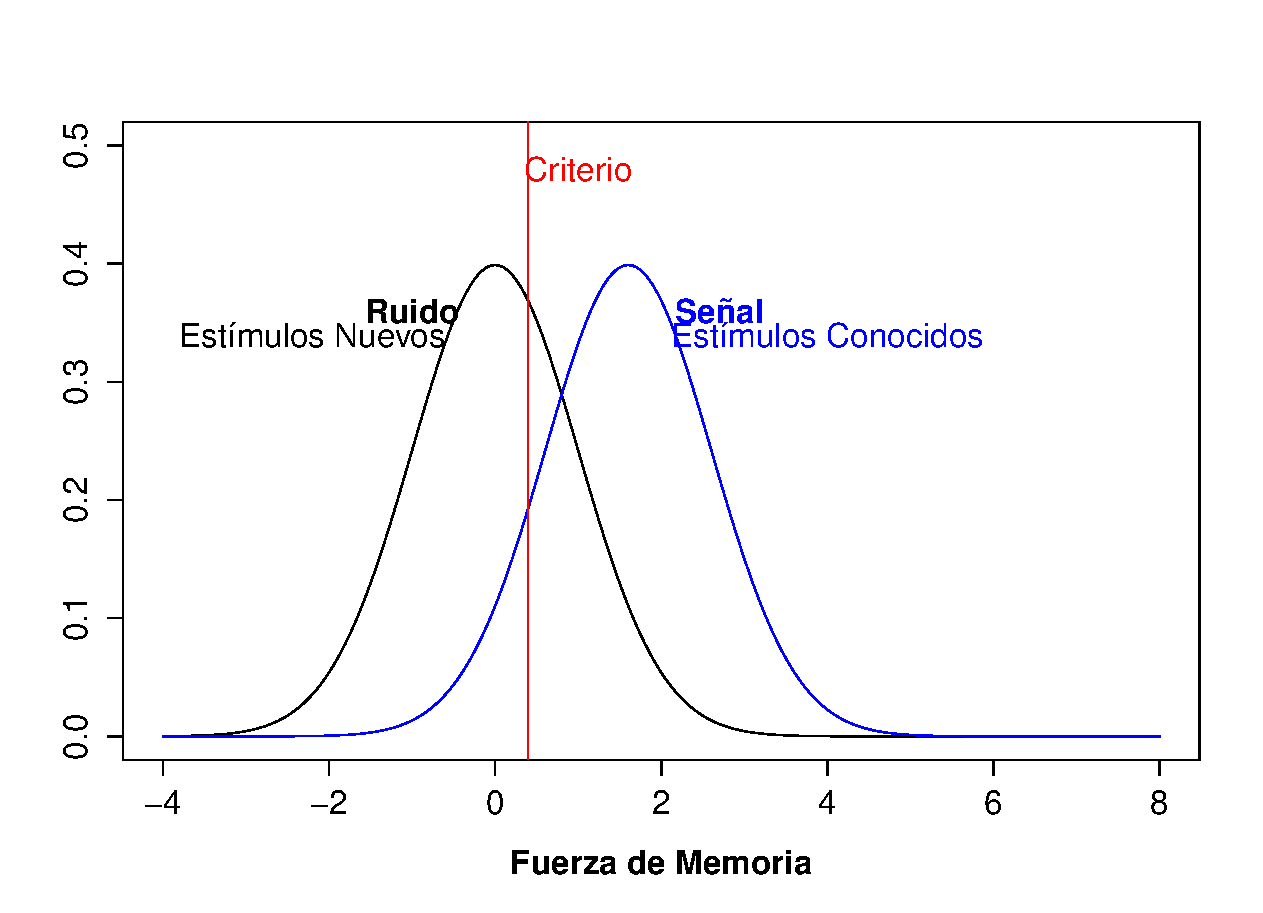
\includegraphics[width=0.60\textwidth]{Figures/RM_SDT_1} 
\decoRule
\caption[SDT en Memoria de Reconocimiento]{Modelo de Detección de Señales aplicado al estudio de Memoria de Reconocimiento}
\label{fig:RM_SDT_1}
\end{figure}

La Figura~\ref{fig:RM_SDT_1} ilustra la forma en que los supuestos de la TDS, expuestos a detalle en el Capítulo 1, se aplican al estudio de la Memoria de Reconocimiento. Las idea central se mantiene en escencia y simplemente sustituimos algunos conceptos: al tratarse de una tarea de reconocimiento, decimos que la 'señal' a detectar es cualquier estímulo antes visto (i.e. 'estímulos viejos', como suelen identificarse en la literatura); el 'ruido' son los estímulos nuevos, que podrían -o no- confundirse con los primeros; el 'eje de decisión' a lo largo del cual se sitúan las dos distribuciones de ruido y señal, se convierte en un 'eje de familiaridad' que va a representar distintos grados de lo que parece ser una 'fuerza de memoria'. También se mantienen las ideas centrales propuestas por el modelo: los estímulos ya antes vistos tendrán valores más altos de 'familiaridad' que aquellos nunca antes vistos, admitiendo sin embargo la posibilidad de que éstos últimos puedan llegar a confundirse con los estímulos viejos, por ejemplo, si comparten algun rasgo en particular; una vez más, dicha variabilidad en la presentación y lectura de los estímulos a evaluar se refleja en la idea de que existen distintos rangos de familiaridad que pueden ser producidos por los estímulos viejos o conocidos, con cierta distribución de probabilidad. Y de la misma forma, la emisión de un juicio se entiende como resultado de comparar la 'familiaridad' de cada estímulo a evaluar con un criterio de elección particular, donde sólo si éste se rebasa, se juzga el estímulo como 'ya antes visto'.\\

Como se mencionó en el Capítulo 1, la TDS en su forma típica define las distribuciones de ruido y señal como distribuciones Gaussianas con varianzas iguales (i.e. con una misma desviación estándar). A propósito de ello, podemos hablar de una particularidad que tiene la aplicaicón de la TDS a estudios de memoria de reconocimiento, que ha sido constante y consistentemente demostrada con los datos: la distribución de Estímulos Viejos suele mostrar mayor desviación estándar que la distribución de Ruido, justo como se muestra en la Figura~\ref{fig:RM_SDT_2}.\\


\begin{figure}[th]
\centering
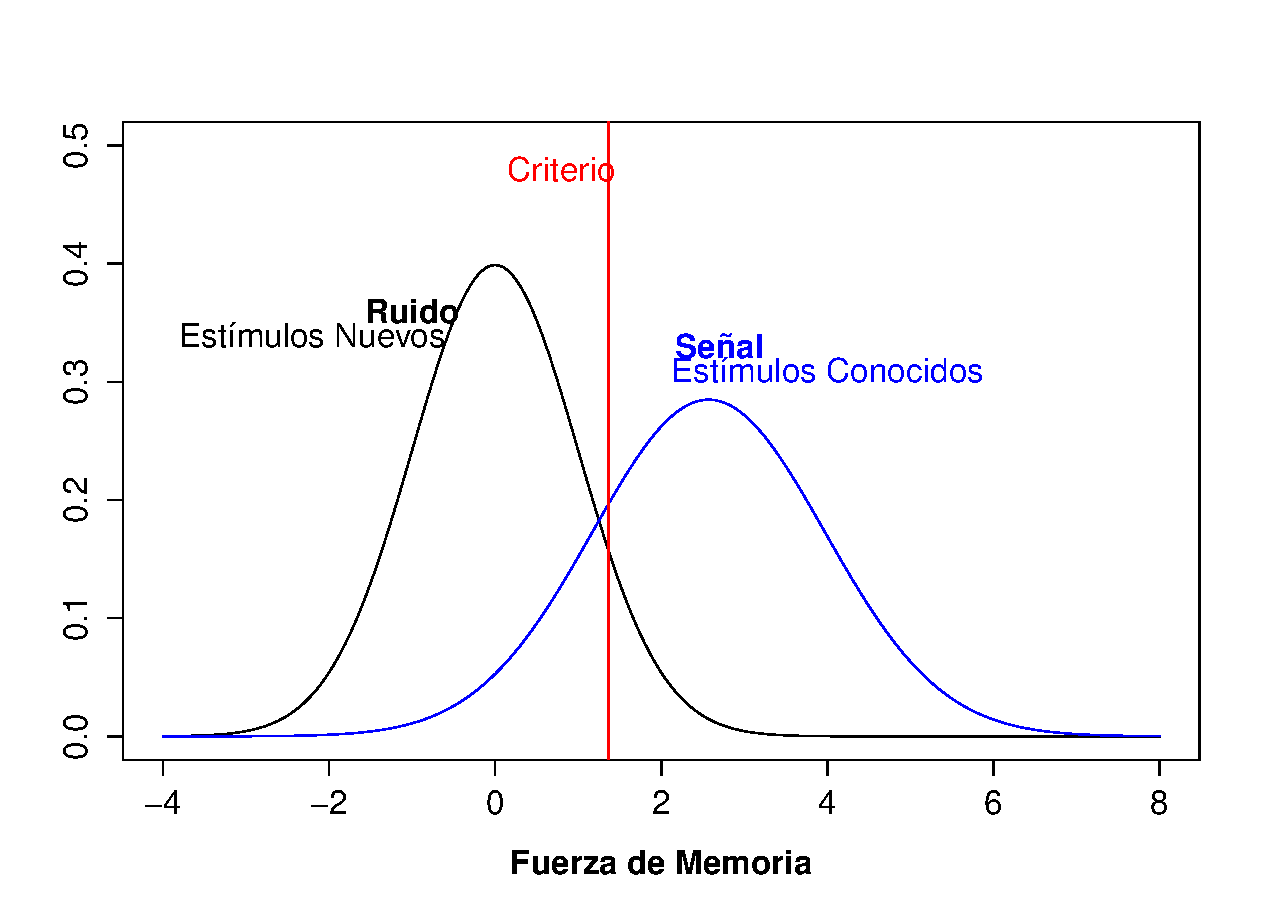
\includegraphics[width=0.60\textwidth]{Figures/RM_SDT_2} 
\decoRule
\caption[SDT en Memoria de Reconocimiento (Varianzas Desiguales)]{Modelo de Detección de Señales con varianzas desiguales aplicado al estudio de Memoria de Reconocimiento}
\label{fig:RM_SDT_2}
\end{figure}


\section{Conflicto entre modelos}

Me permitiré, por un momento, salirme del molde académico y hablar un poco de todo el proceso que hubo detrás de la realización del presente trabajo. Cuando comencé a revisar literatura para decidir cuál podría ser mi proyecto de tesis, descubrí la maravilla de la Teoría de Detección de Señales. 

Sin embargo, pese a la flexibilidad de la que dispone la TDS para aplicarse a, aparentemente, cualquier tarea de decisión binaria, donde se admita el papel de la incertidumbre en la emisión de un juicio de detección, su aplicación al campo de la Memoria de Reconocimiento no ha estado excenta de críticas.

Conceptualmente, es fácil pensar en una tarea de reconocimiento en términos del modelo de detección de señales. Sin embargo, cuando se revisan las implicaciones teóricas que conllevaría aceptar que la memoria de Reconocimiento funciona como un procedimiento cualquiera de detección de señales, no son del todo claras. 

\subsection{Proceso Dual Detección de Señales - Umbral alto}

Ante el conflicto existen siempre distintos caminos y estilos de afrontamiento. La TDS ha sido vista como antagonista directa de los modelos de Procesamiento Dual en tanto que define el problema del reconocimiento como dependiente de un sólo proceso de comparación de la familiaridad percibida con un criterio de elección del sistema. Existe una amplia literatura, que discutiremos más adelante, que se ha enfocado en poner a prueba dichos modelos para comparar directamente su poder.

Una estrategia diferente para resolver este conflicto entre la TDS y el Procesamiento Dual es hacer a un lado la recolección de evidencia que pudiera otorgar a uno de los dos enfoques en competencia la victoria definitiva para concentrarse en la conciliación de estos modelos, ya sea desde el plano conceptual, o bien, a partir del desarrollo de un nuevo modelo unificador.

Por ejemplo, en una serie de experimentos presentados por \parencite{Atkinson1973}, 



\subsection{}

Una vía alterna para solucionar el conflcitoque se tiene con 







%----------------------------------------------------------------------------------------
%	SECTION 2
%----------------------------------------------------------------------------------------

\section{El Efecto Espejo}


 
% Chapter Template

\chapter{El Efecto Espejo: Implicaciones y Aproximaciones} % Main chapter title

\label{Cap_ME} % Change X to a consecutive number; for referencing this chapter elsewhere, use \ref{ChapterX}

%----------------------------------------------------------------------------------------
%	SECTION 1
%----------------------------------------------------------------------------------------

\section{Evidencia recolectada}

Lorem ipsum dolor sit amet, consectetur adipiscing elit. Aliquam ultricies lacinia euismod. Nam tempus risus in dolor rhoncus in interdum enim tincidunt. Donec vel nunc neque. In condimentum ullamcorper quam non consequat. Fusce sagittis tempor feugiat. Fusce magna erat, molestie eu convallis ut, tempus sed arcu. Quisque molestie, ante a tincidunt ullamcorper, sapien enim dignissim lacus, in semper nibh erat lobortis purus. Integer dapibus ligula ac risus convallis pellentesque.



\subsection{Relevancia}
Morbi rutrum odio eget arcu adipiscing sodales. Aenean et purus a est pulvinar pellentesque. Cras in elit neque, quis varius elit. Phasellus fringilla, nibh eu tempus venenatis, dolor elit posuere quam, quis adipiscing urna leo nec orci. Sed nec nulla auctor odio aliquet consequat. Ut nec nulla in ante ullamcorper aliquam at sed dolor. Phasellus fermentum magna in augue gravida cursus. Cras sed pretium lorem. Pellentesque eget ornare odio. Proin accumsan, massa viverra cursus pharetra, ipsum nisi lobortis velit, a malesuada dolor lorem eu neque.

%-----------------------------------
%	SUBSECTION 1
%-----------------------------------
\subsection{Algunos modelos desarrollados para dar cuenta del Efecto Espejo}

Nunc posuere quam at lectus tristique eu ultrices augue venenatis. Vestibulum ante ipsum primis in faucibus orci luctus et ultrices posuere cubilia Curae; Aliquam erat volutpat. Vivamus sodales tortor eget quam adipiscing in vulputate ante ullamcorper. Sed eros ante, lacinia et sollicitudin et, aliquam sit amet augue. In hac habitasse platea dictumst.

%-----------------------------------
%	SUBSECTION 2
%-----------------------------------



%----------------------------------------------------------------------------------------
%	SECTION 2
%----------------------------------------------------------------------------------------

\section{Main Section 2}

Sed ullamcorper quam eu nisl interdum at interdum enim egestas. Aliquam placerat justo sed lectus lobortis ut porta nisl porttitor. Vestibulum mi dolor, lacinia molestie gravida at, tempus vitae ligula. Donec eget quam sapien, in viverra eros. Donec pellentesque justo a massa fringilla non vestibulum metus vestibulum. Vestibulum in orci quis felis tempor lacinia. Vivamus ornare ultrices facilisis. Ut hendrerit volutpat vulputate. Morbi condimentum venenatis augue, id porta ipsum vulputate in. Curabitur luctus tempus justo. Vestibulum risus lectus, adipiscing nec condimentum quis, condimentum nec nisl. Aliquam dictum sagittis velit sed iaculis. Morbi tristique augue sit amet nulla pulvinar id facilisis ligula mollis. Nam elit libero, tincidunt ut aliquam at, molestie in quam. Aenean rhoncus vehicula hendrerit.
% Chapter Template

\chapter{Experimento: Buscando el Efecto Espejo en una tarea Perceptual} % Main chapter title

\label{Cap_Exp} % Change X to a consecutive number; for referencing this chapter elsewhere, use \ref{ChapterX}

%----------------------------------------------------------------------------------------
%	SECTION 1
%----------------------------------------------------------------------------------------
\section{Planteamiento general}

%Se propone buscar evidencia del Efecto Espejo en una tarea fuera de Memoria de reconocimiento


%Se propone una tarea perceptual ya que carece de una fase de preparacion
El interés principal del trabajo aquí expuesto es evaluar la posibilidad de que el Efecto Espejo y los patrones de respuesta identificados como parte del mismo, sean un producto del uso del modelo de detección de señales en la comparación del desempeño de los participantes a lo largo de dos condiciones de dificultad cualesquiera y no así de una discrepancia en el grado en que se tratan dichas condiciones a nivel de ciertos procesos superiores de atención y memoria alterando el orden en que dichos estímulos se distribuyen en el eje de la evidencia. Para ello se diseñó una tarea de detección meramente perceptual, donde las condiciones de dificultad fueron construidas con base en su discriminabilidad perceptual. 

%Se trabaja con ilusiones opticas, dado que la literatura en ellas permite anticiparnos a la d' y proponer dos niveles de dificultad.
Las ilusiones ópticas constituyen un fenómeno atractivo para la psicología cognoscitiva interesada en el estudio de nuestr os sistemas perceptuales, en tanto que han permitido dar evidencia de cómo se puede engañar a dichos sistemas 

%De encontrarse el efecto espejo, se sugeriría que éste es un producto de la aplicación del TDS y no así de procesos superiores.

\subsection{Objetivo}

%Buscar evidencia del efecto espejo en una tarea de detección que no implique el reconocimiento de estimulos ya conocidos.
Poner a prueba la existencia de los patrones de respuesta identificados como parte del Efecto Espejo en una tarea de detección perceptual con dos niveles de dificultad, (i.e. una tarea de detección que no pertenezca a la familia de tareas de reconocimiento y, principalmente, que carezca de una etapa previa a la fase experimental donde los participantes tuvieran ocasión de manipular los estímulos y hacer alguna distinción entre niveles de dificultad).


\section{Construcción de la Tarea}

Por tratarse de estímulos no antes probados en una tarea de detección como la aquí propuesta, se decidió correr dos experimentos que bien podrían pensarse como dos variaciones del mismo procedimiento experimental. 

De acuerdo a \parencite{Massaro1971}, la 

\subsection{Estímulos}

\begin{itemize}
\item Experimento 1 : Circulo de referencia aislado vs Figura de Ebbinghaus
\item Experimento 2 : Dos figuras de Ebbinghaus
\end{itemize}


Las figuras de Ebbinghaus construidas de acuerdo a un diseño factorial de 5x2x2 (Ver Figura). 

\subsection{Materiales}
La tarea fue programada y ejecutada a partir de Psychopy v.12. Se controló que la distancia que separase los estímulos presentados se encontrara dentro de un ángulo de $X grados$ del campo visual de los participantes, así como que estos realizaran la tarea en una distancia de 1 m respecto del monitor.

\subsection{Participantes}

Un total de cuarenta y un estudiantes de la Facultad de Psicología participaron en alguno de los dos experimentos presentados; el Experimento 1 se llevó a cabo con veinte participantes y el Experimento 2, con veintiuno. Ambos experimentos se llevaron a cabo simultáneamente por lo que la asignación de los participantes a cualquiera de los mismos se hizo de manera alternada, procurando garantizar que la muestra de parti

\section{Procedimiento}



\subsection{Registro de respuestas}

El experimento fue programado de manera tal que por cada participante se obtuviera un documento en formato csv (i.e. comma separated value) que contuviera información, ensayo a ensayo, sobre la respuesta dada por 
 
% Chapter Template

\chapter{Datos: Sólo datos.} % Main chapter title

\label{Cap_Data} % Change X to a consecutive number; for referencing this chapter elsewhere, use \ref{ChapterX}

%----------------------------------------------------------------------------------------
%	SECTION 1
%----------------------------------------------------------------------------------------
\section{Explorando la ejecución de los participantes}

En este capítulo se presentan de manera gráfica los datos obtenidos para cada participante en cada uno de los experimentos realizados. 

\subsection{Control 1: ¿Los participantes estaban poniendo atención a la tarea?}




%%%%%%%%%%%%%%%%%%%%%%%%%%%%%%%%%%%%%%%%%%%%%%%%%%%%%%%%%%%%%%
%%%%%%%%%  Respuesta (Y/N) en los ensayos
% Experimento 2
%%%%%%%%%%%%%%%%%%%%%%%%%%%%%%%%%%%%%%%%%%%%%%%%%%%%%%%%%%%%%%%
\begin{figure}[th]
\centering
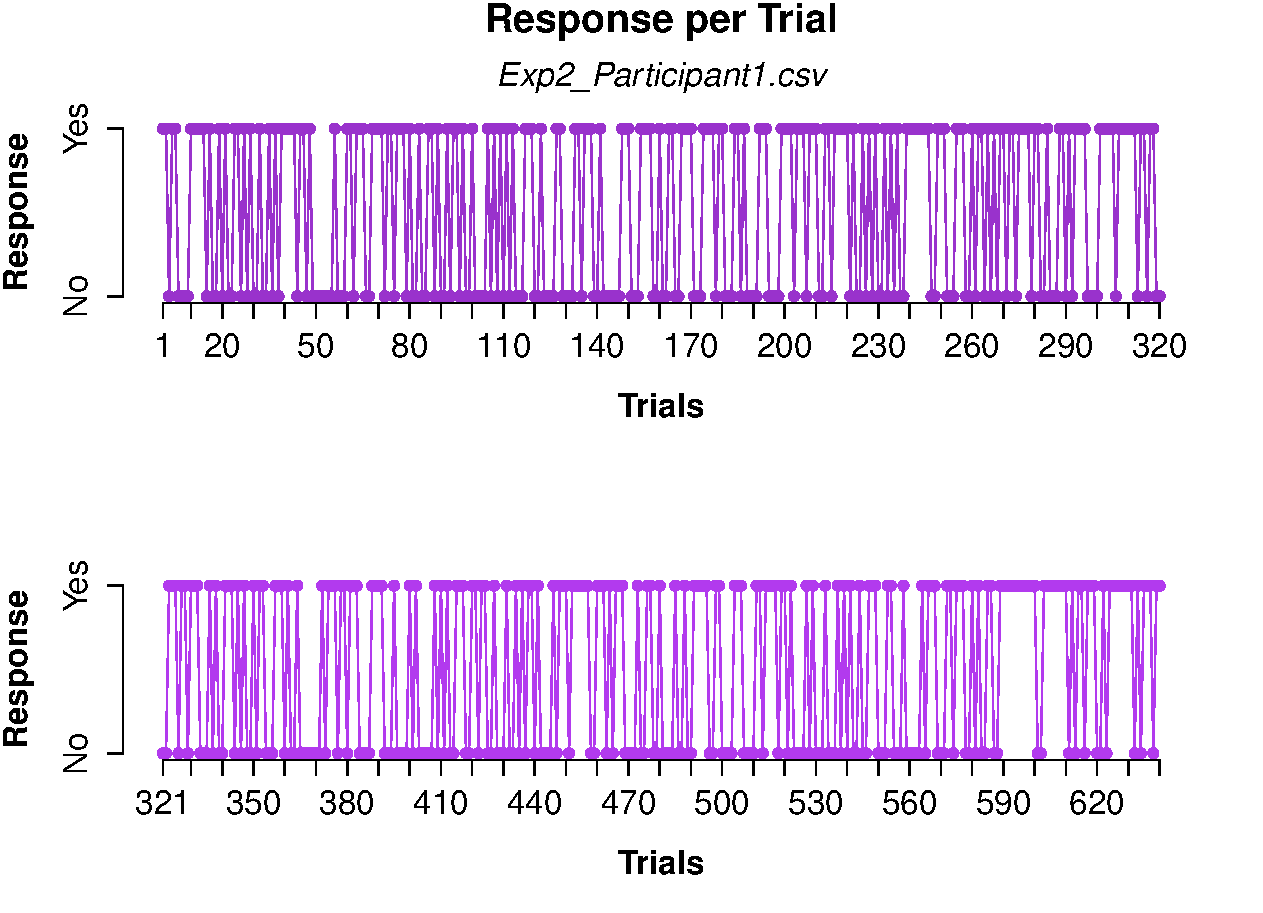
\includegraphics[width=0.30\textwidth]{Figures/Response_Exp2_P1} 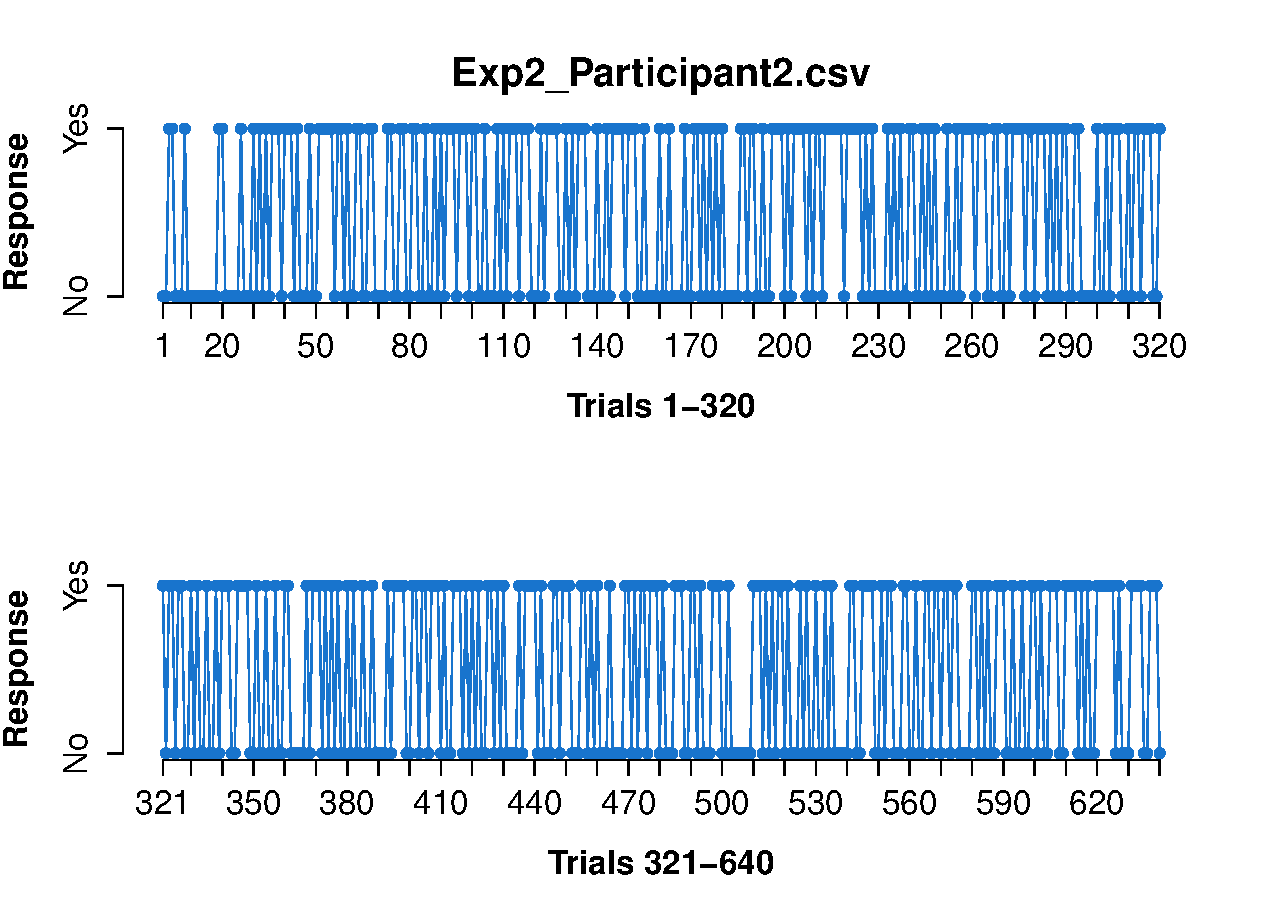
\includegraphics[width=0.30\textwidth]{Figures/Response_Exp2_P2} 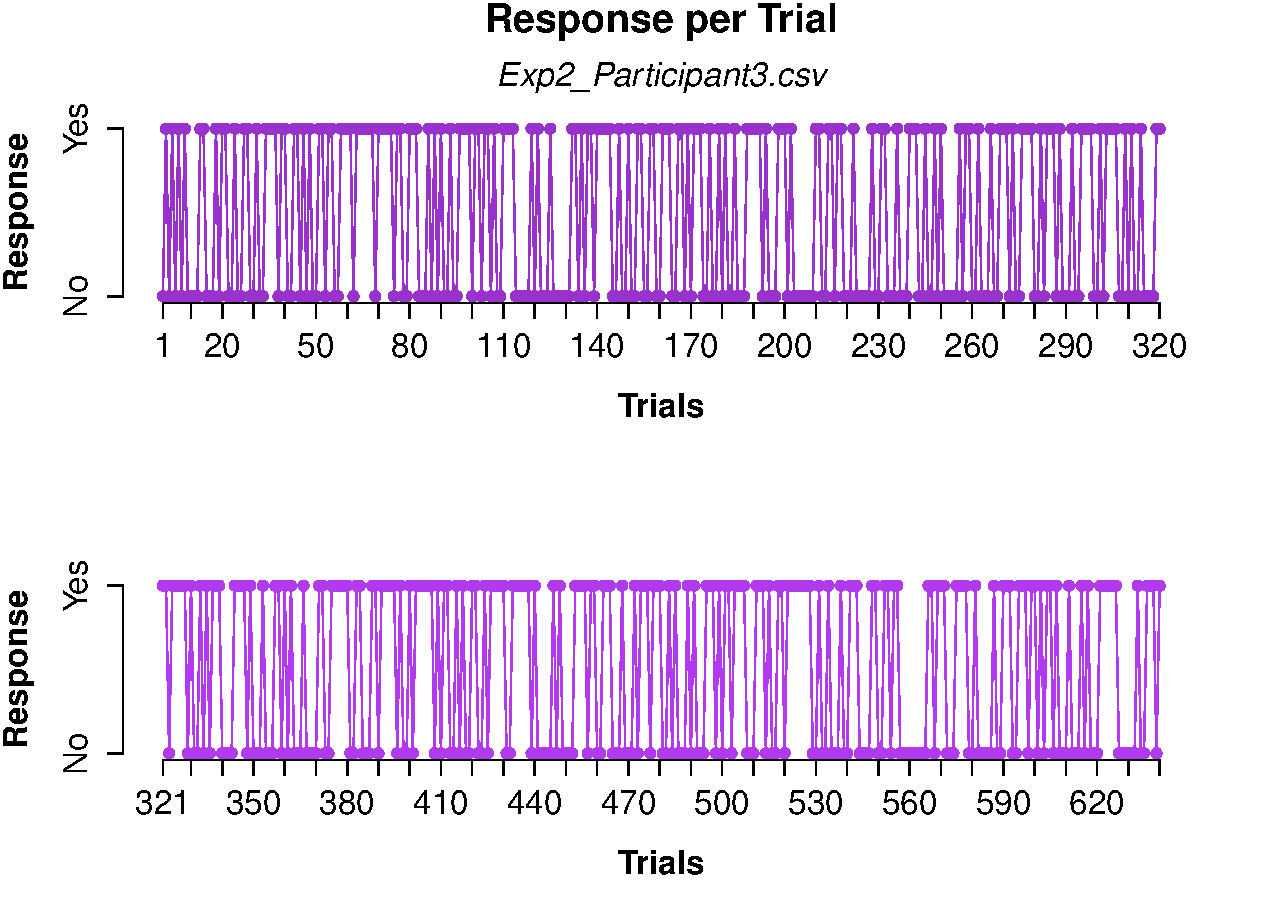
\includegraphics[width=0.30\textwidth]{Figures/Response_Exp2_P3}
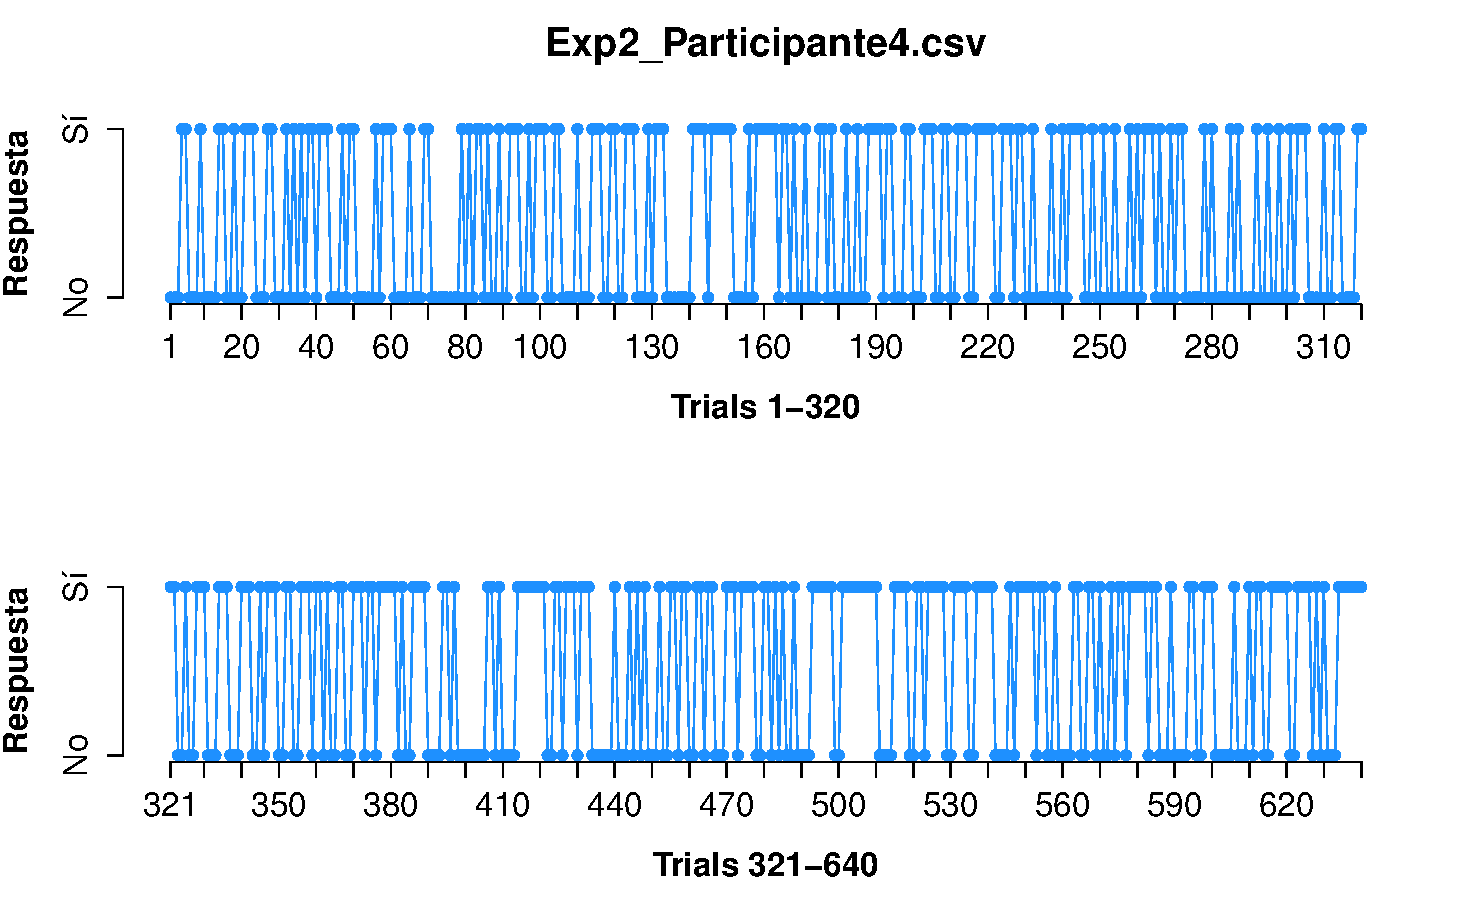
\includegraphics[width=0.30\textwidth]{Figures/Response_Exp2_P4} 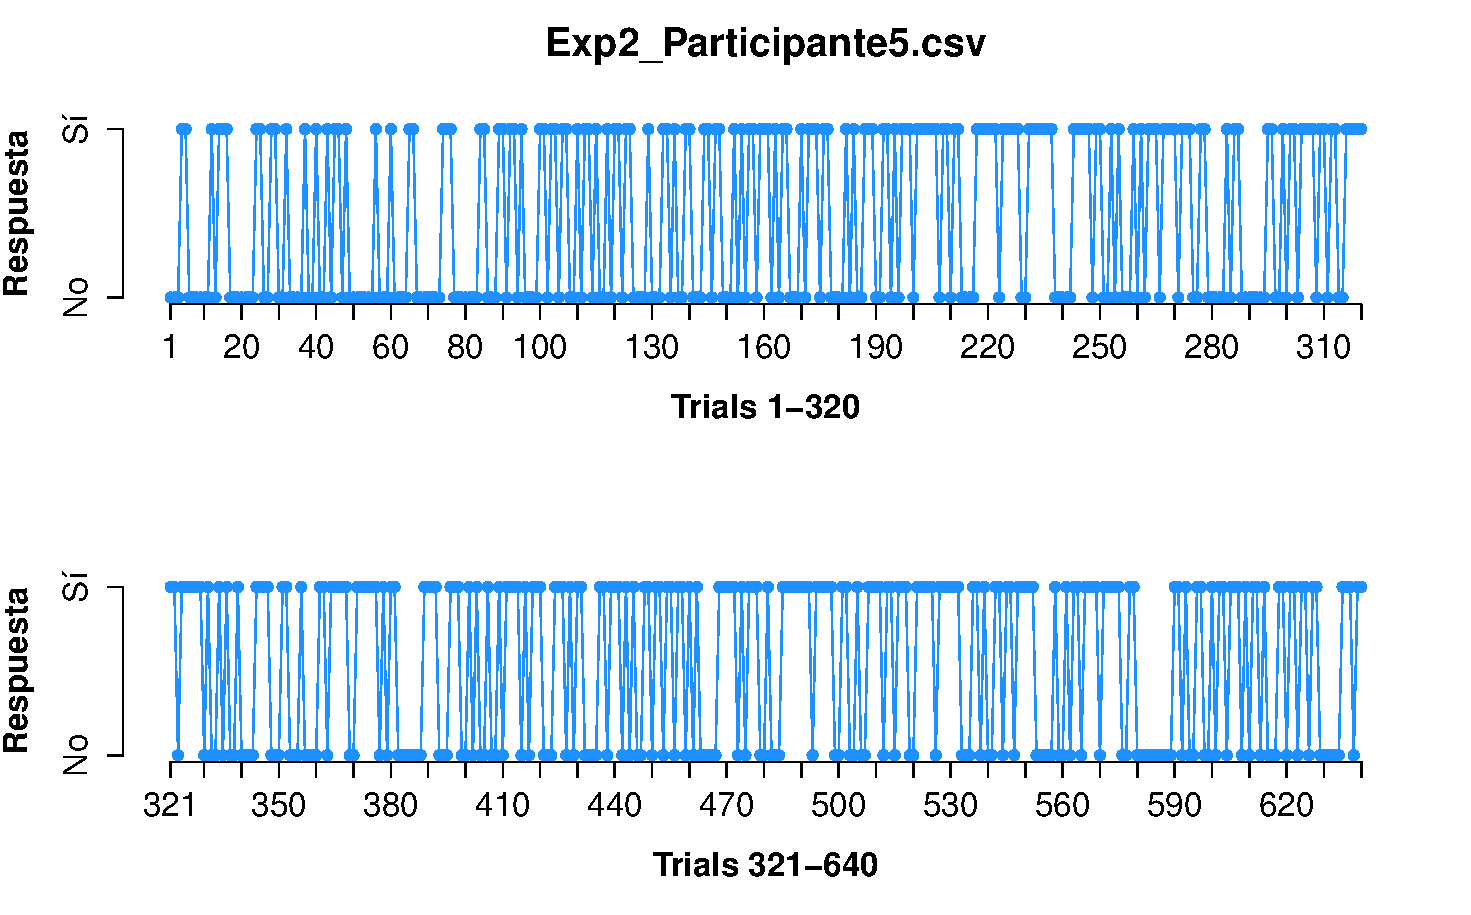
\includegraphics[width=0.30\textwidth]{Figures/Response_Exp2_P5} 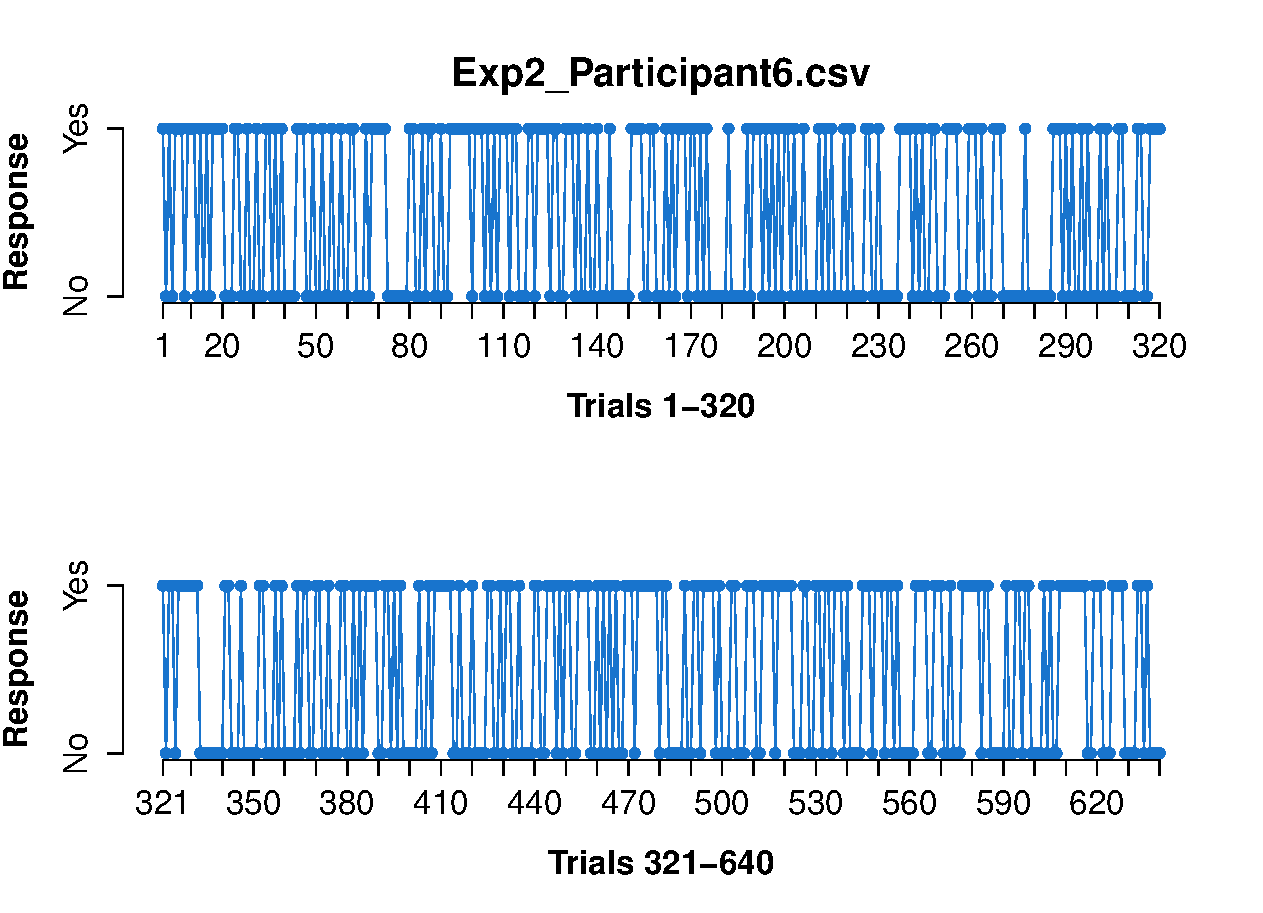
\includegraphics[width=0.30\textwidth]{Figures/Response_Exp2_P6}
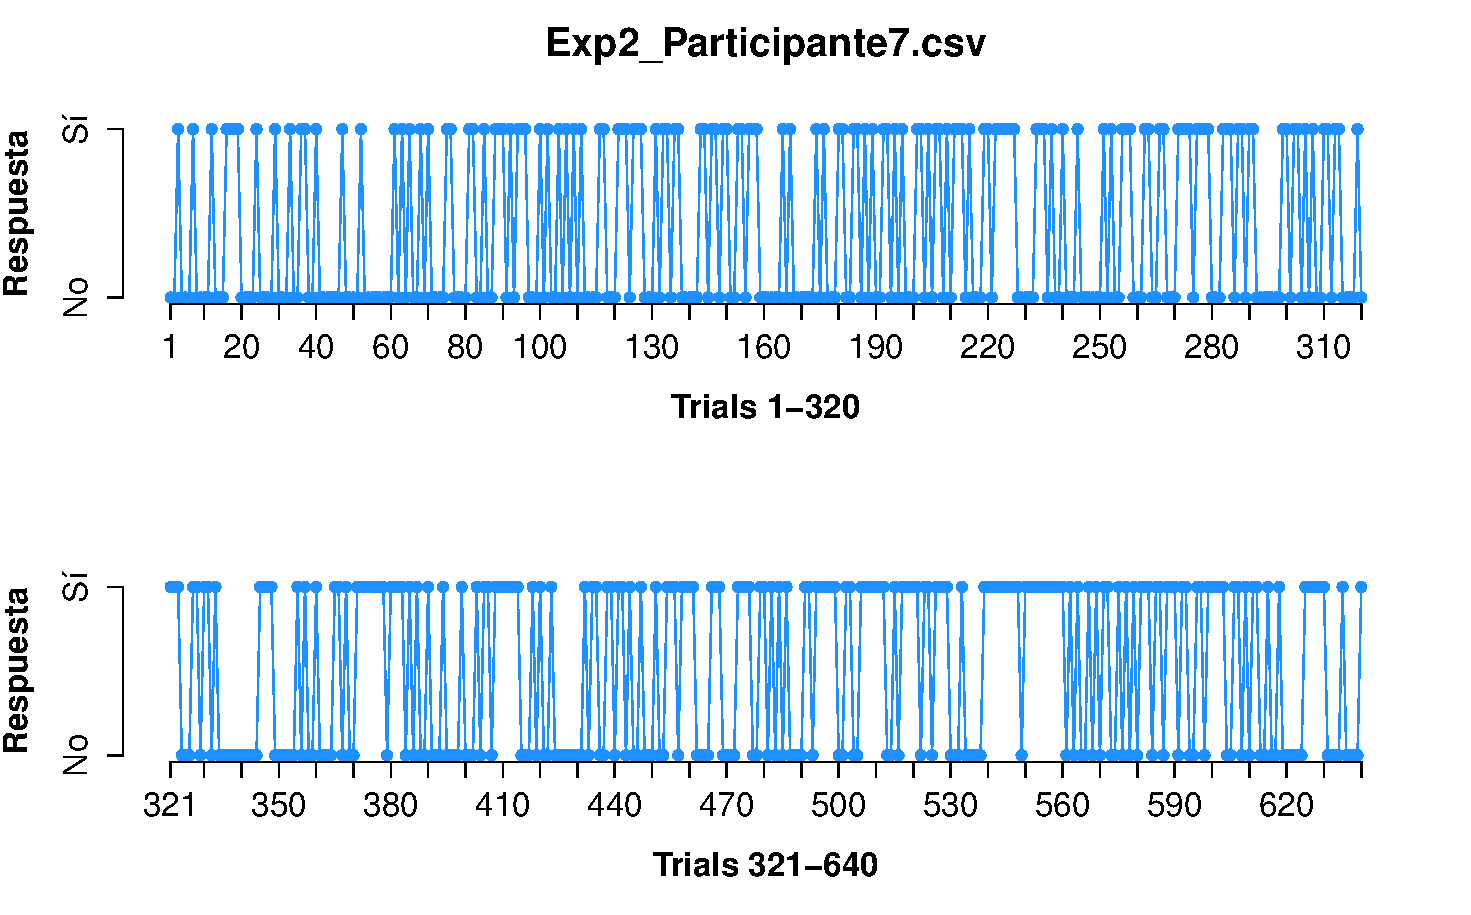
\includegraphics[width=0.30\textwidth]{Figures/Response_Exp2_P7} 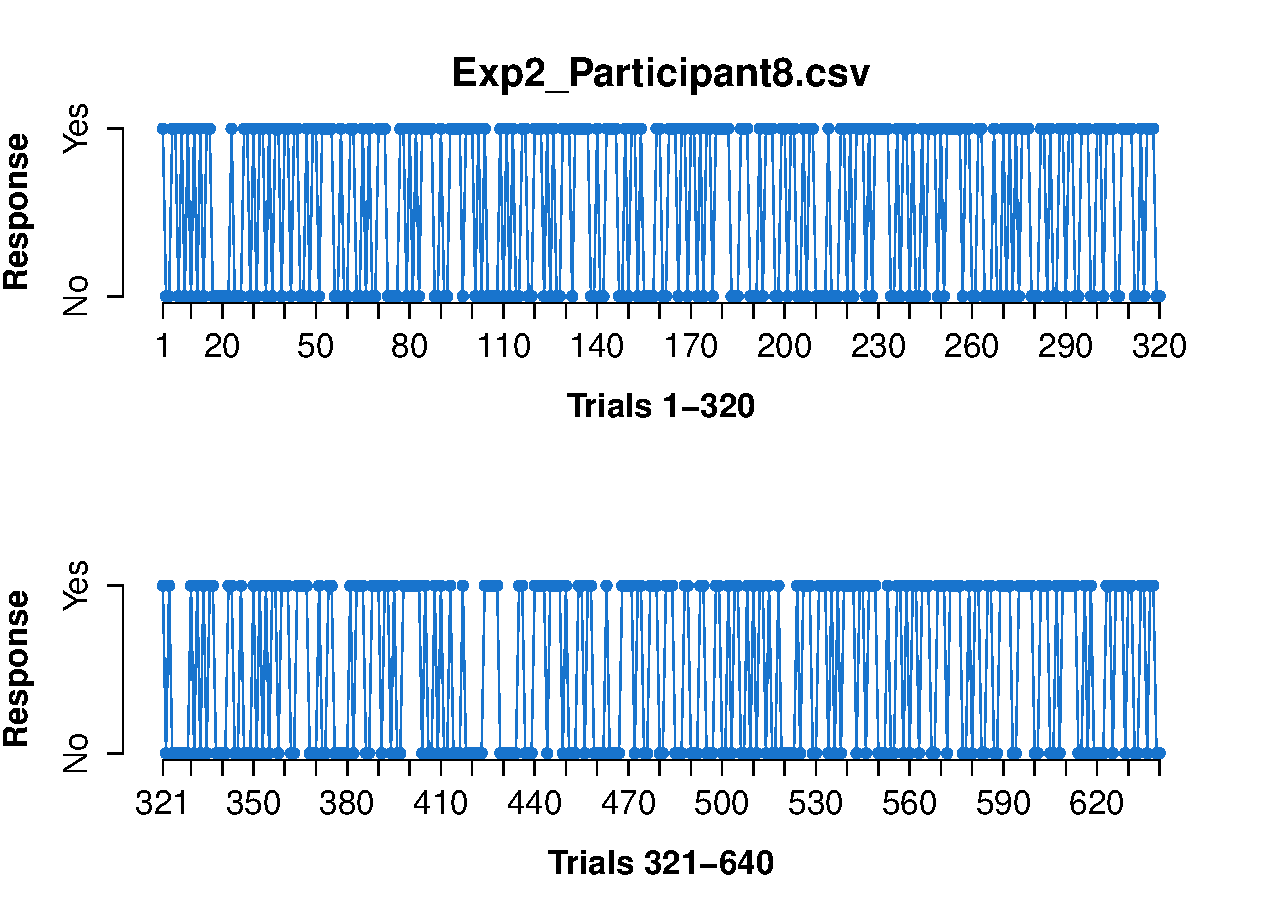
\includegraphics[width=0.30\textwidth]{Figures/Response_Exp2_P8} 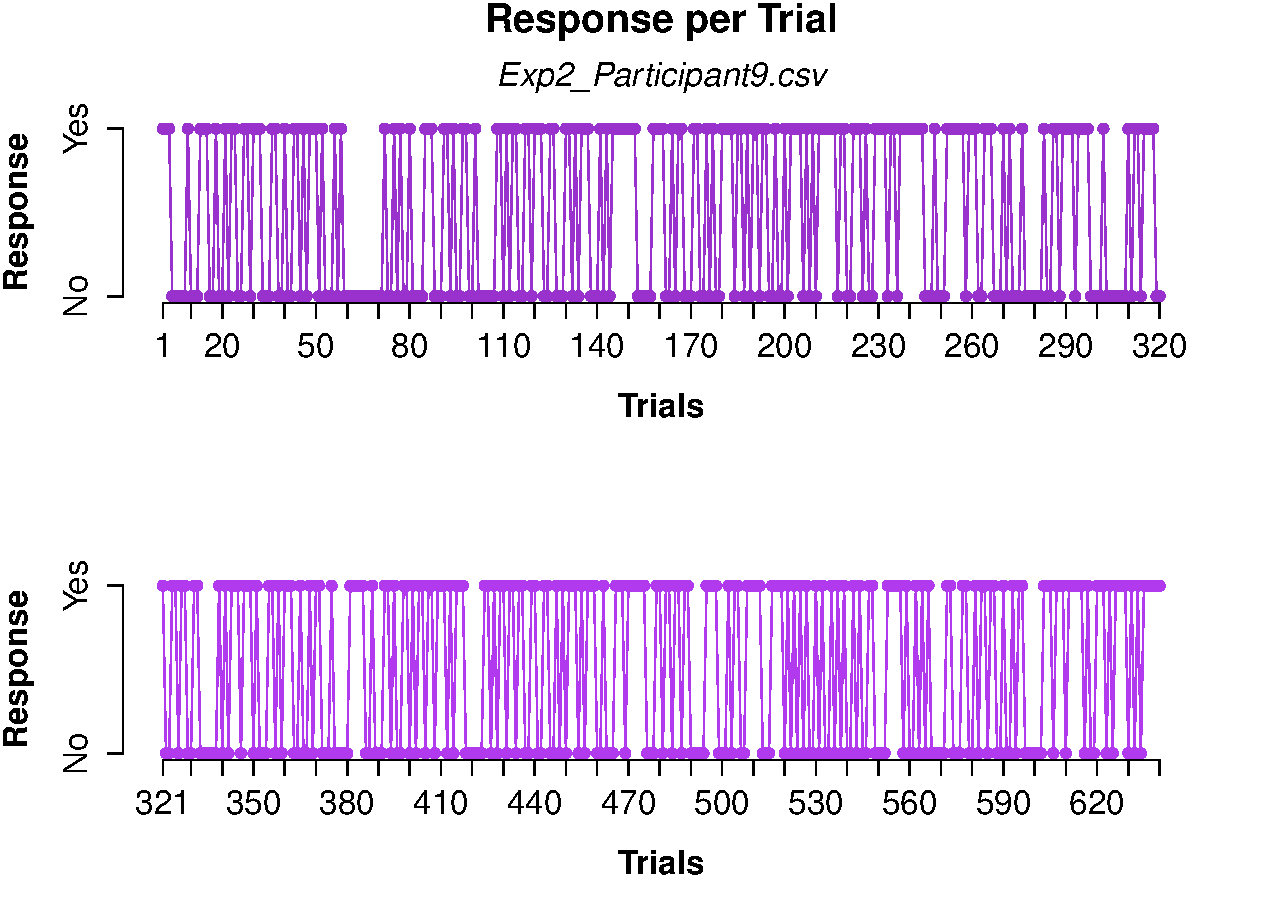
\includegraphics[width=0.30\textwidth]{Figures/Response_Exp2_P9}
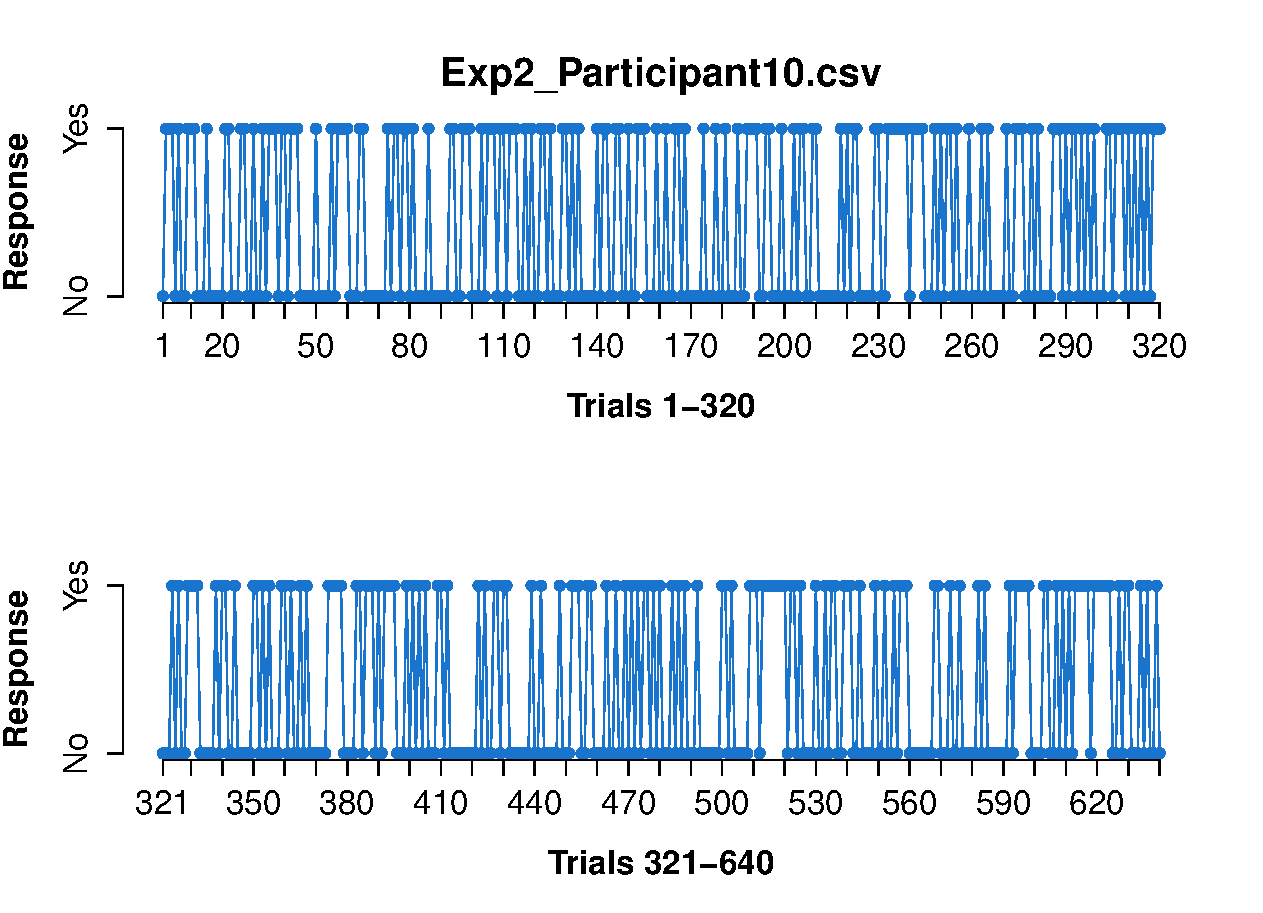
\includegraphics[width=0.30\textwidth]{Figures/Response_Exp2_P10} 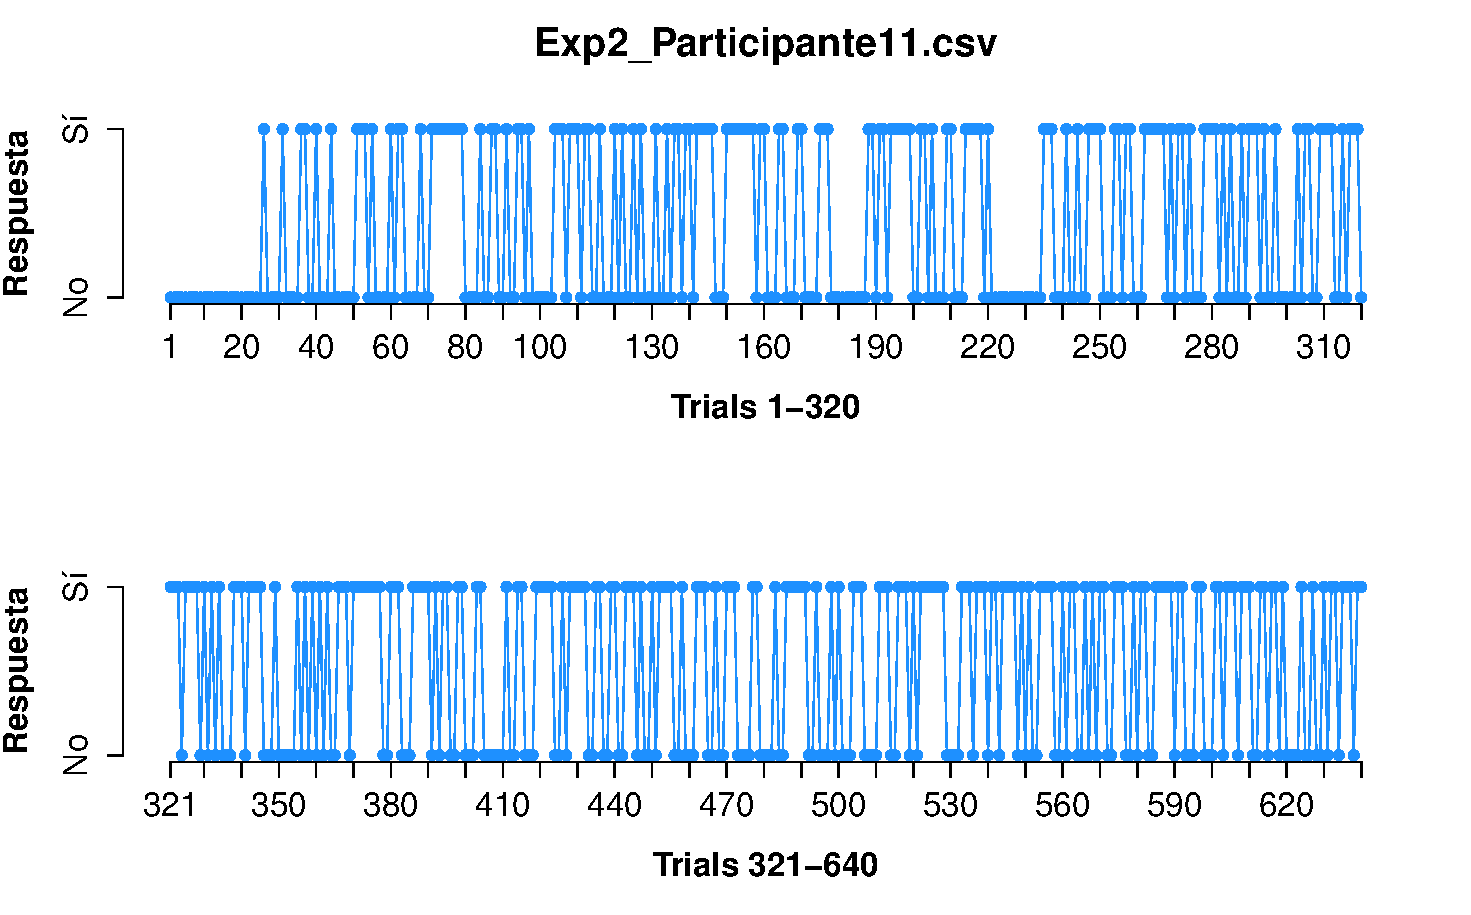
\includegraphics[width=0.30\textwidth]{Figures/Response_Exp2_P11} 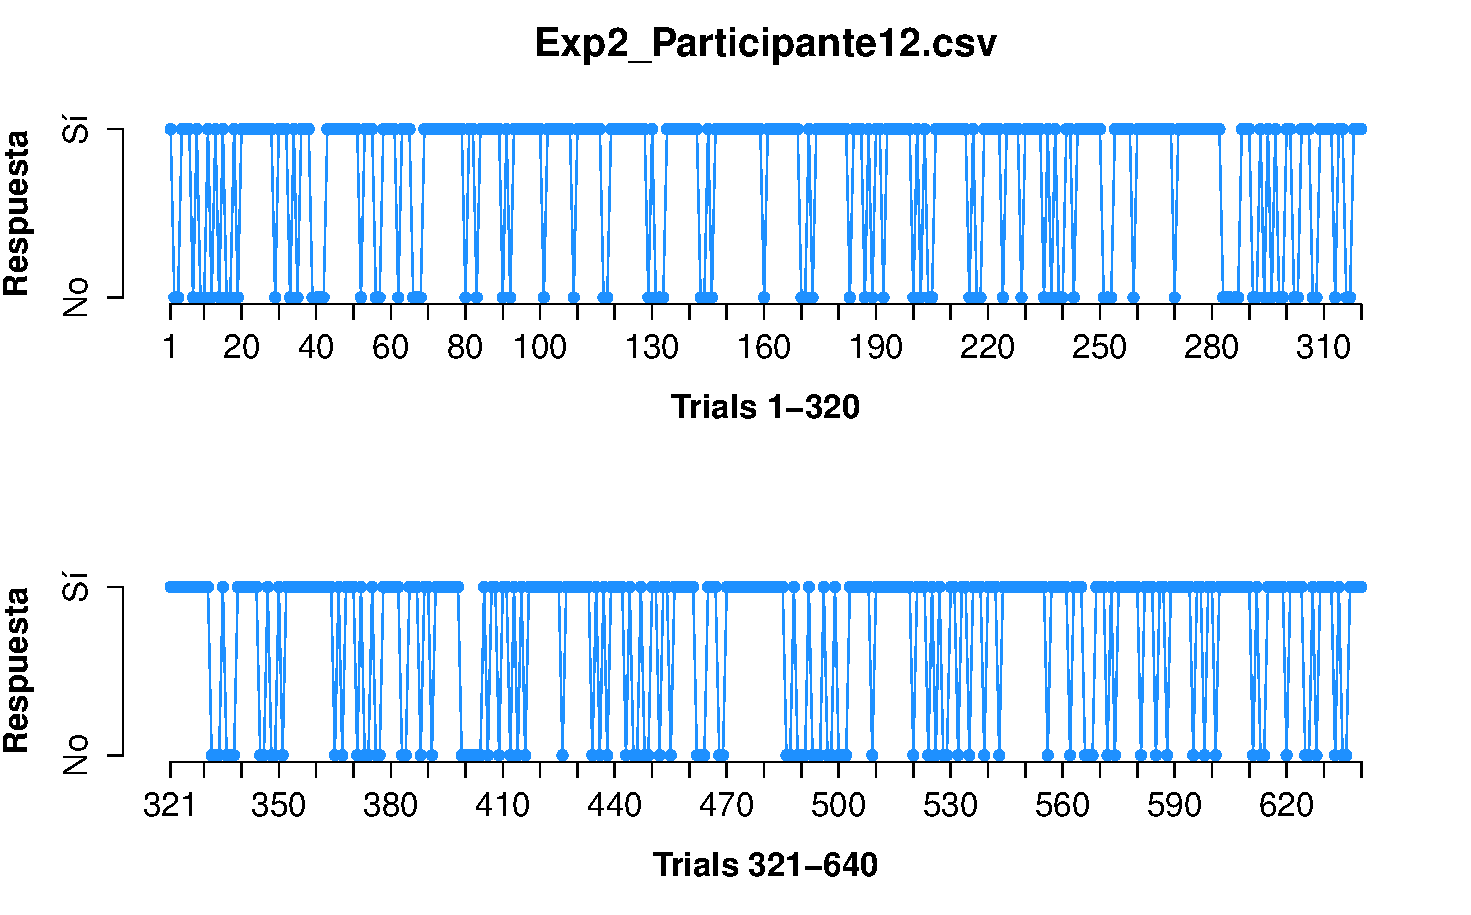
\includegraphics[width=0.30\textwidth]{Figures/Response_Exp2_P12}
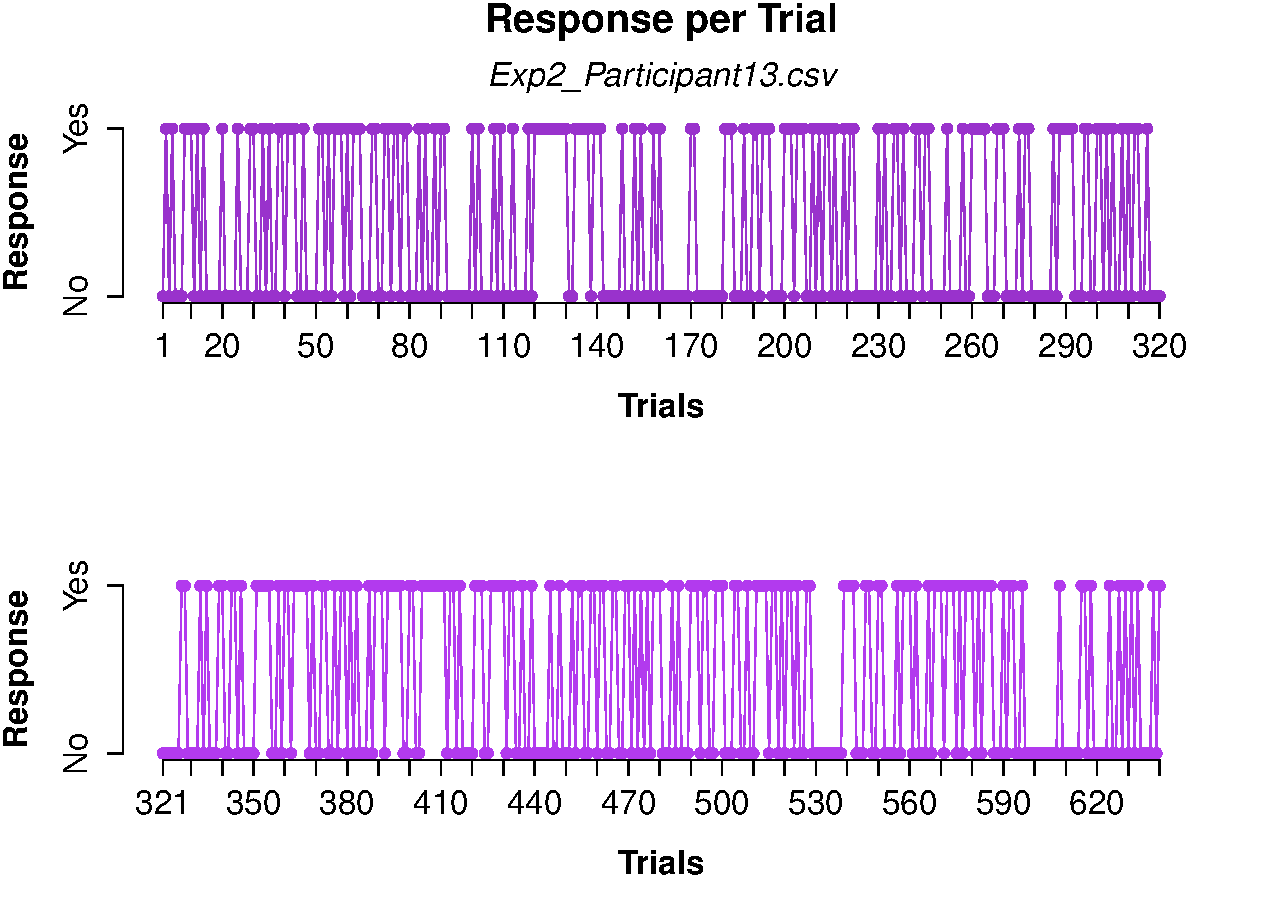
\includegraphics[width=0.30\textwidth]{Figures/Response_Exp2_P13} 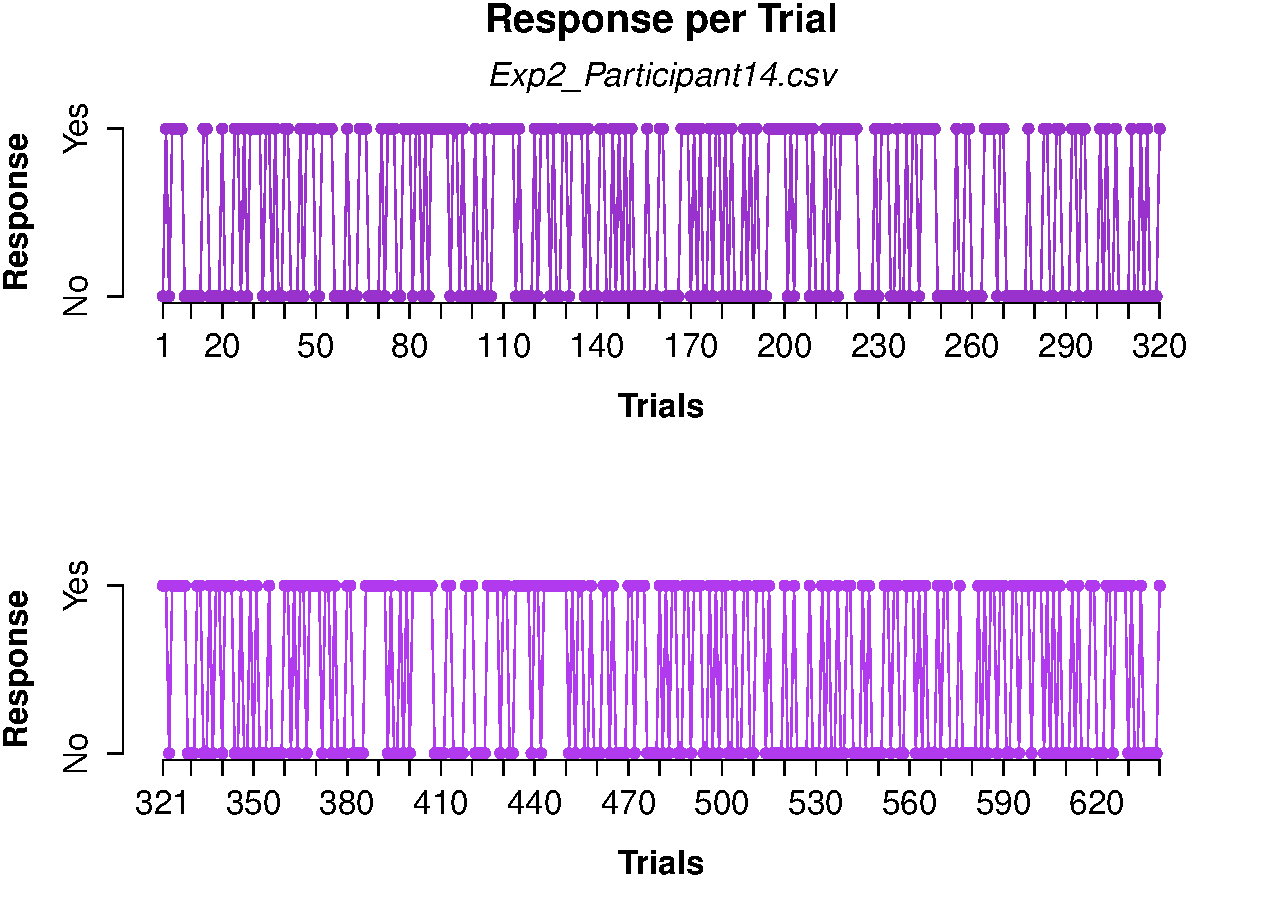
\includegraphics[width=0.30\textwidth]{Figures/Response_Exp2_P14} 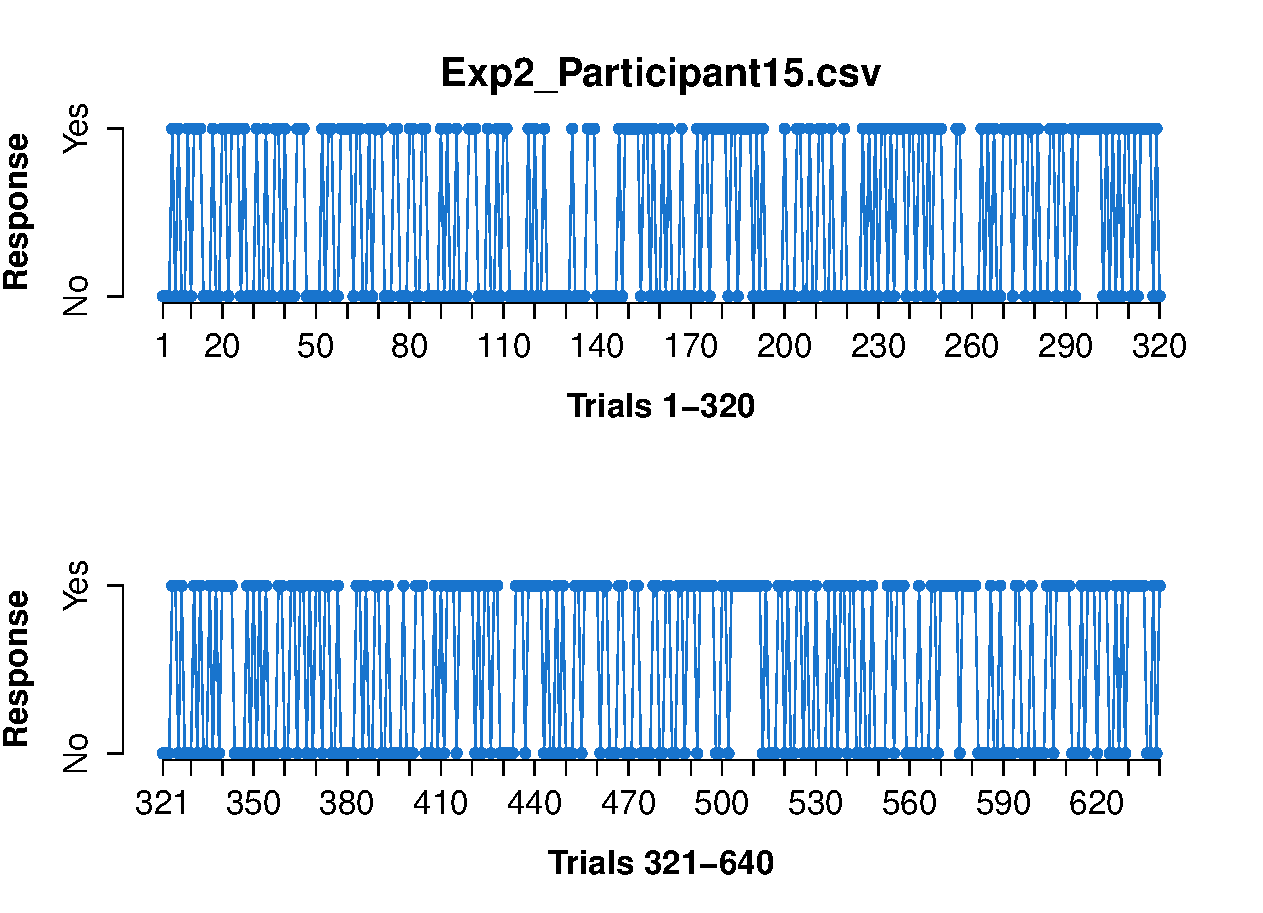
\includegraphics[width=0.30\textwidth]{Figures/Response_Exp2_P15}
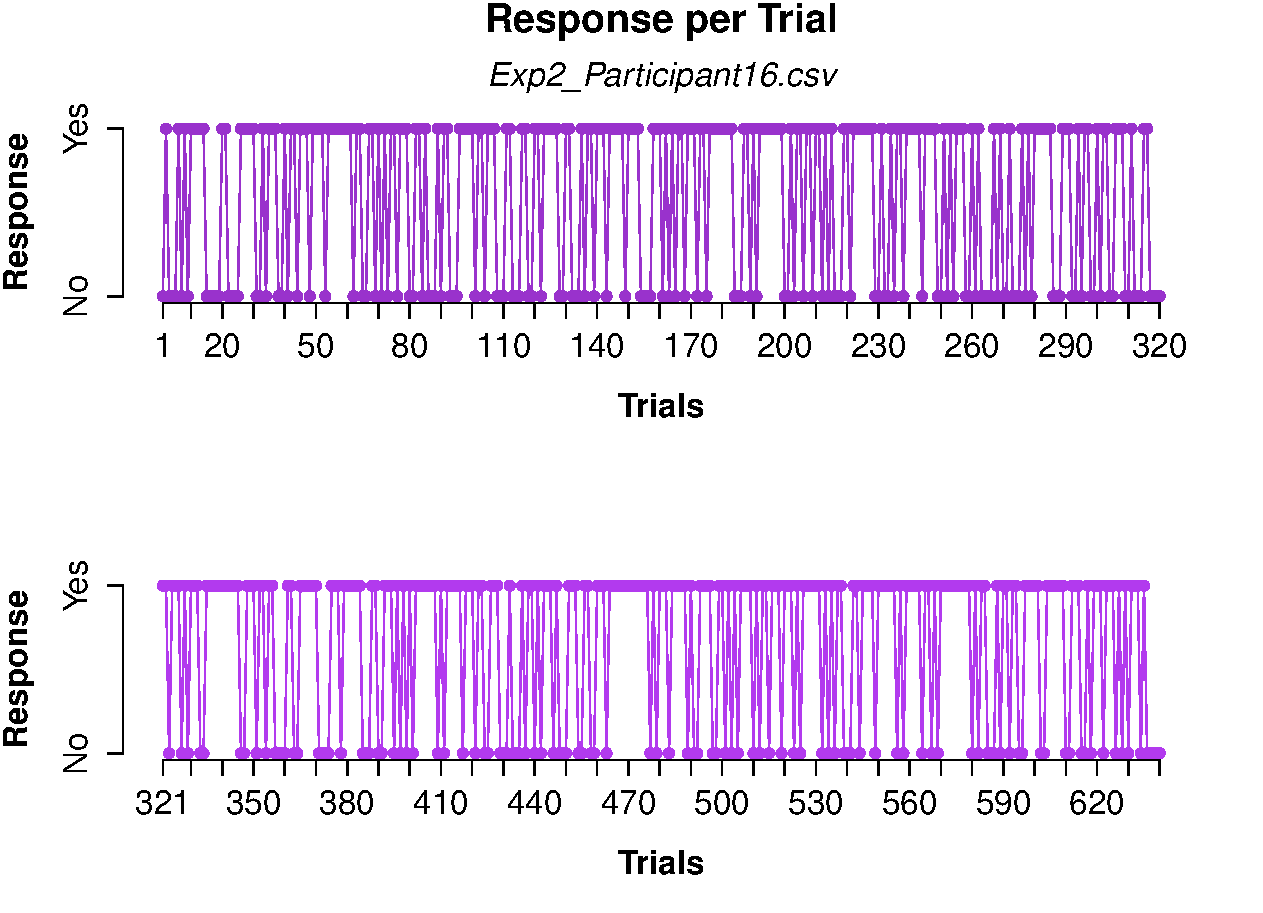
\includegraphics[width=0.30\textwidth]{Figures/Response_Exp2_P16} 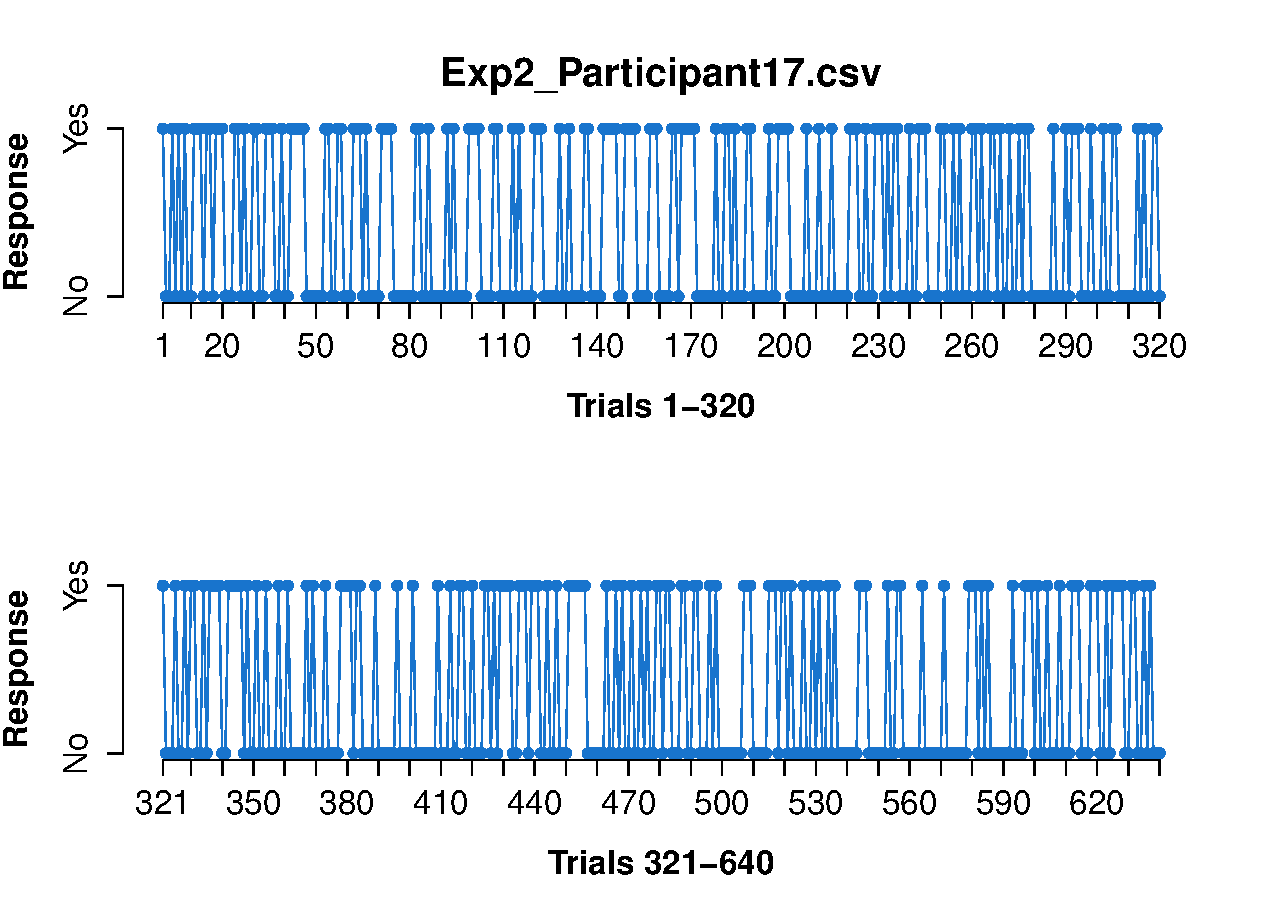
\includegraphics[width=0.30\textwidth]{Figures/Response_Exp2_P17} 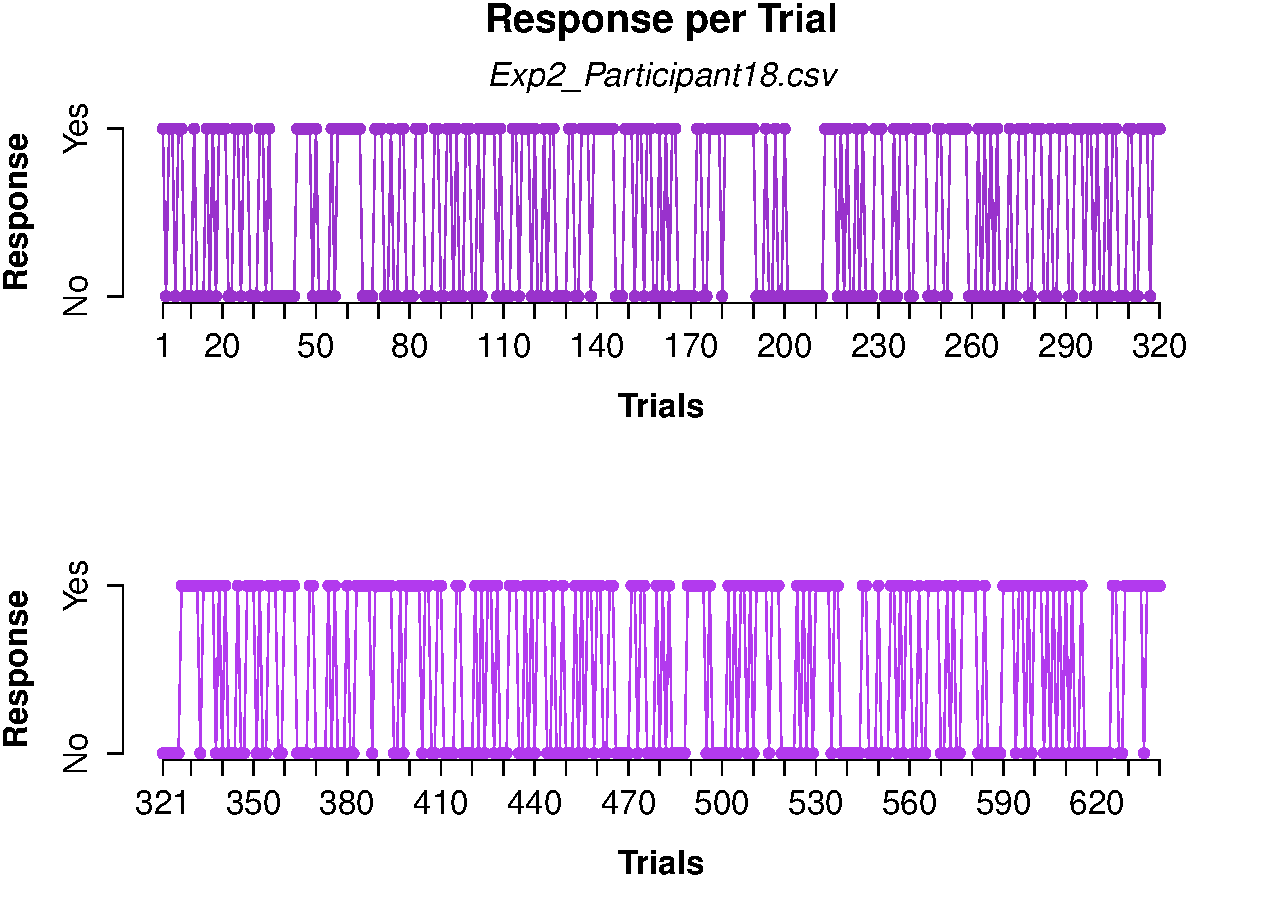
\includegraphics[width=0.30\textwidth]{Figures/Response_Exp2_P18}
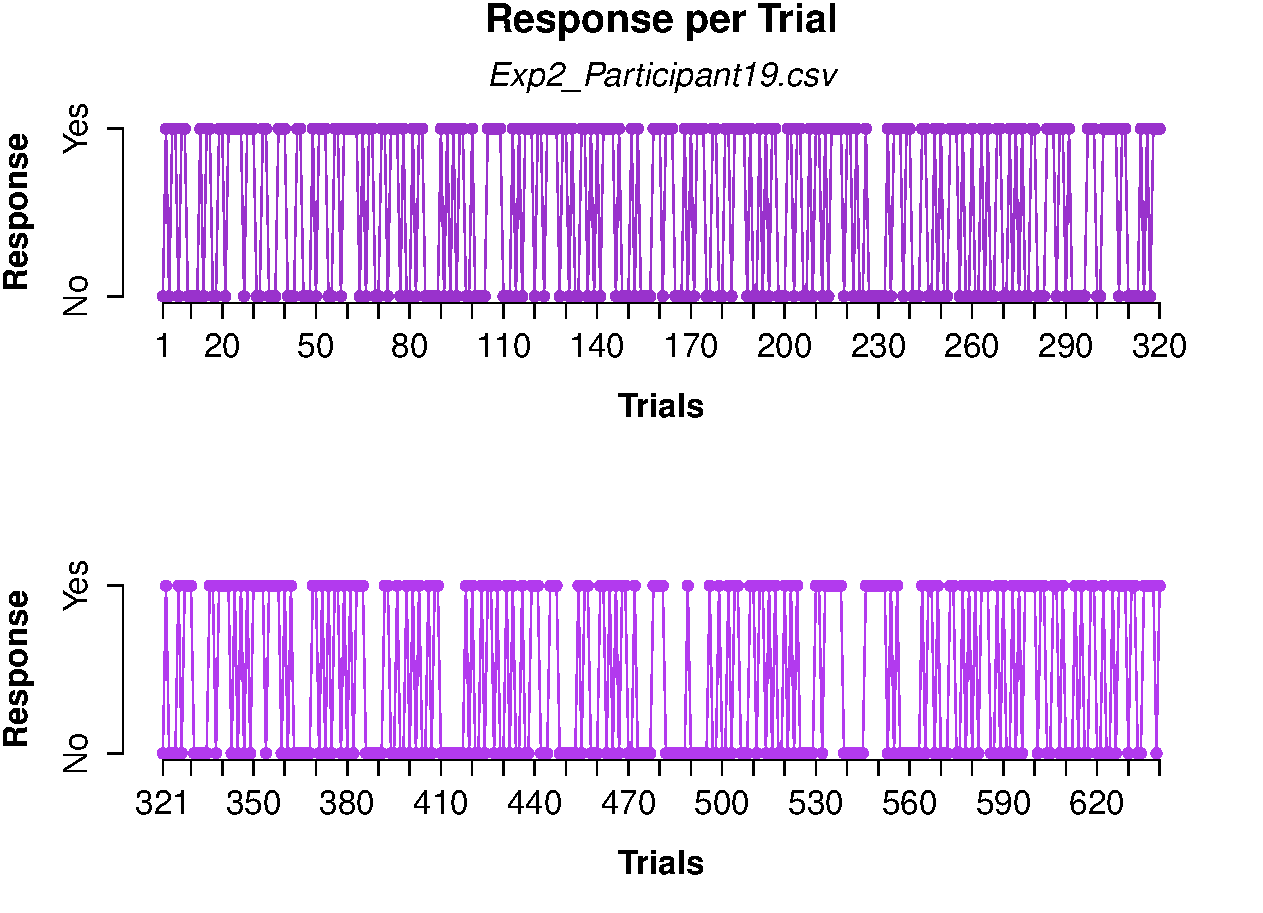
\includegraphics[width=0.30\textwidth]{Figures/Response_Exp2_P19} 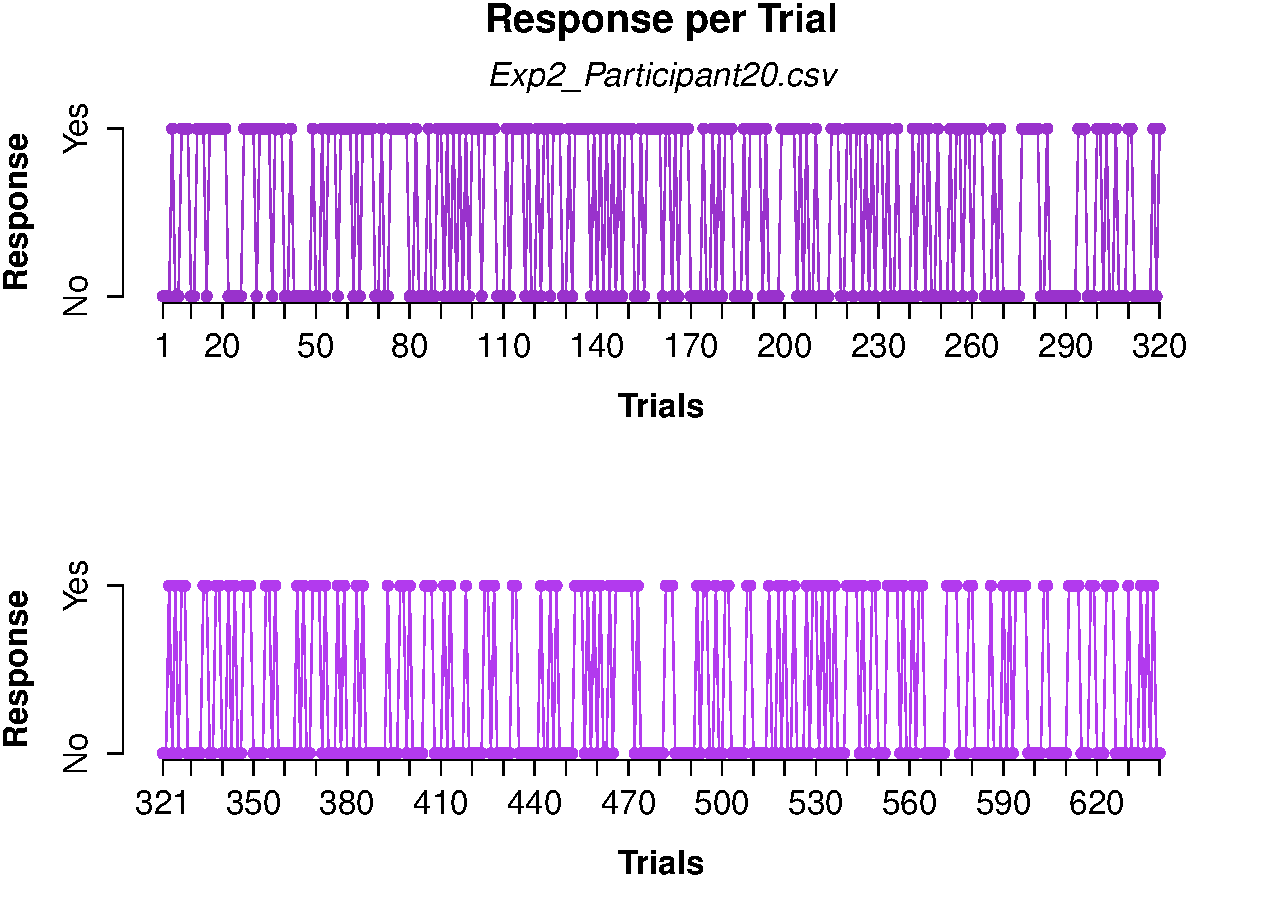
\includegraphics[width=0.30\textwidth]{Figures/Response_Exp2_P20} 
%\decoRule
\caption[Response_Exp2]{Respuesta por ensayo (Experimento 2).}
\label{fig:Response_E2}
\end{figure}




%%%%%%%%%%%%%%%%%%%%%%%%%%%%%%%%%%%%%%%%%%%%%%%%%%%%%%%%%%%%%%
%%%%%%%%%  Respuesta Rating en los ensayos
% Experimento 2
%%%%%%%%%%%%%%%%%%%%%%%%%%%%%%%%%%%%%%%%%%%%%%%%%%%%%%%%%%%%%%%
\begin{figure}[th]
\centering
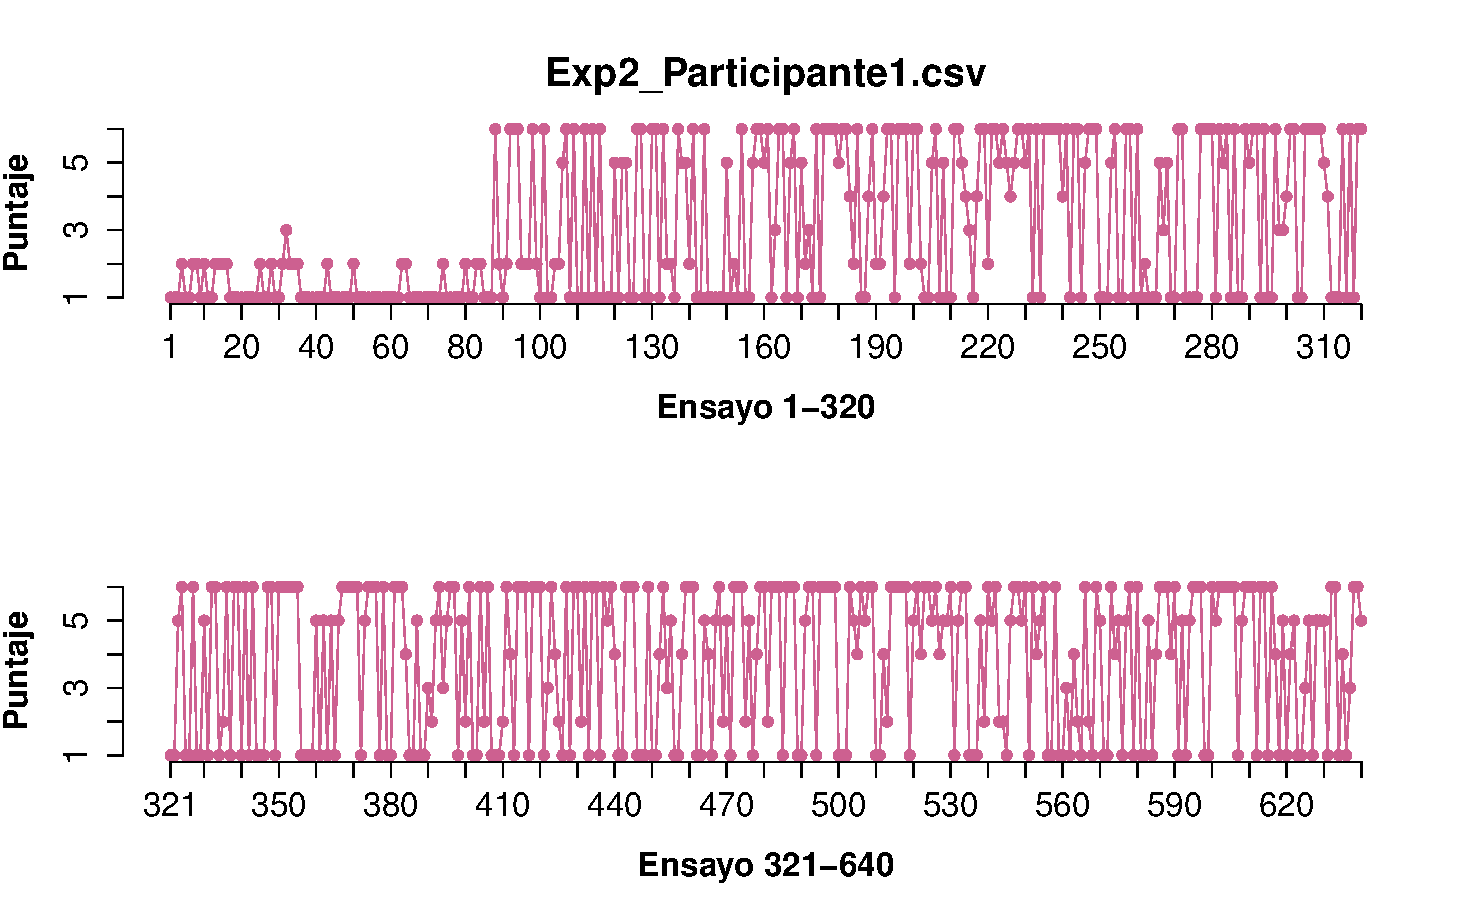
\includegraphics[width=0.30\textwidth]{Figures/Rating_Exp2_P1} 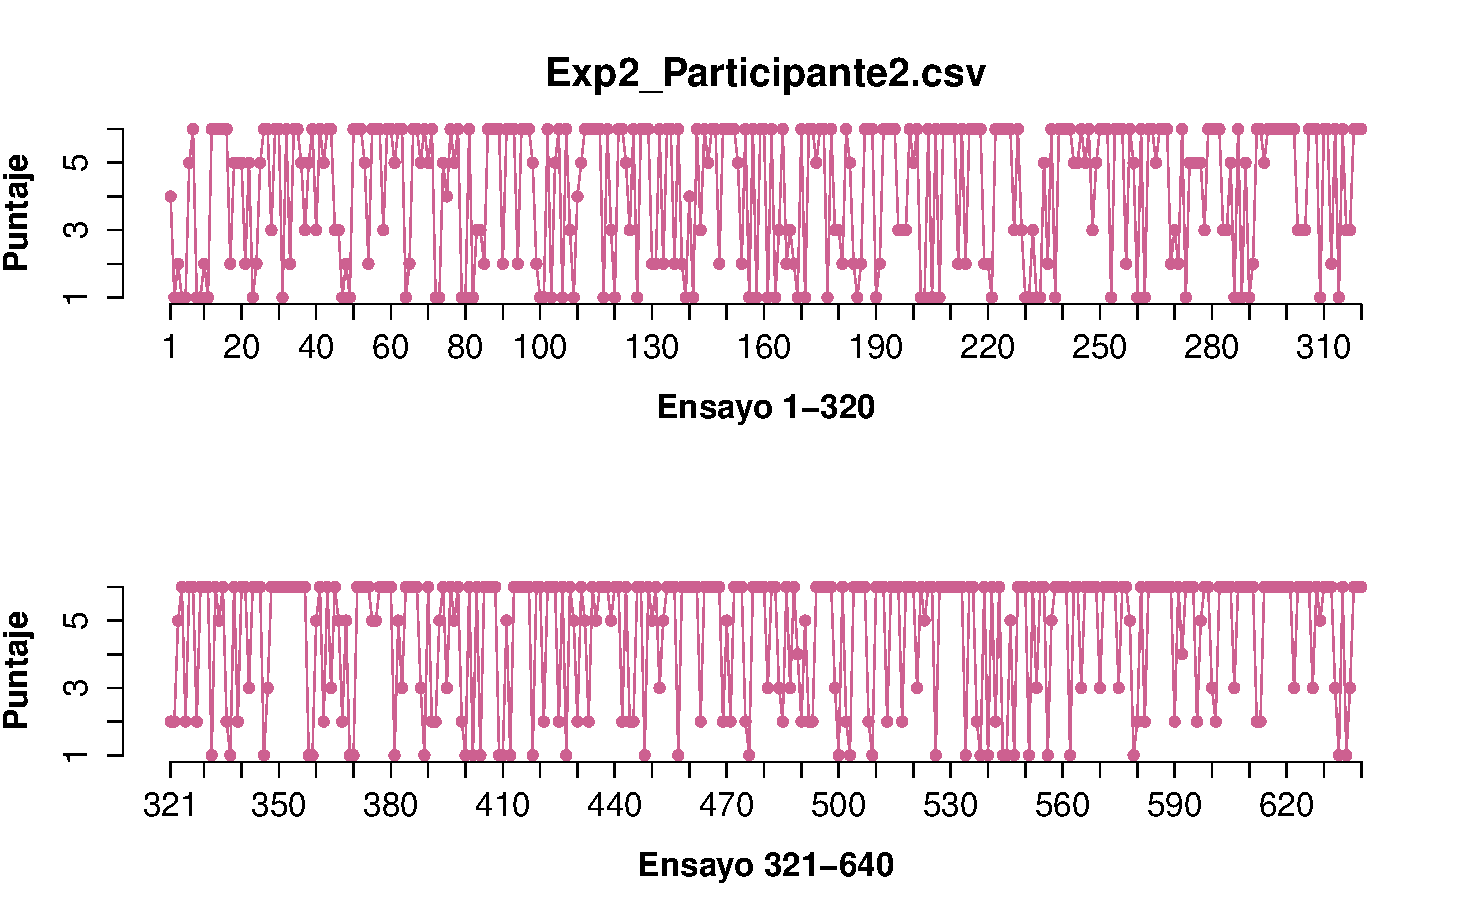
\includegraphics[width=0.30\textwidth]{Figures/Rating_Exp2_P2} 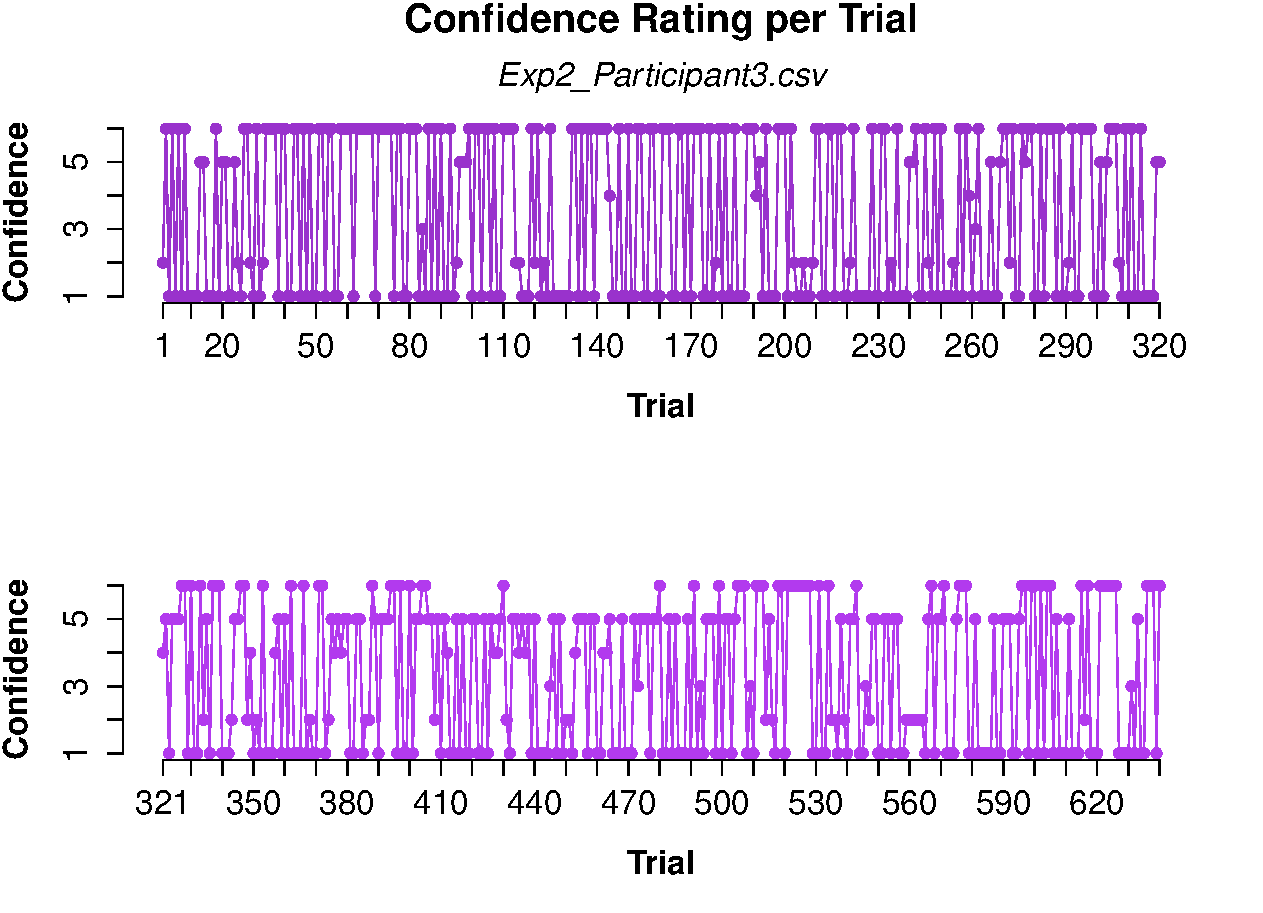
\includegraphics[width=0.30\textwidth]{Figures/Rating_Exp2_P3}
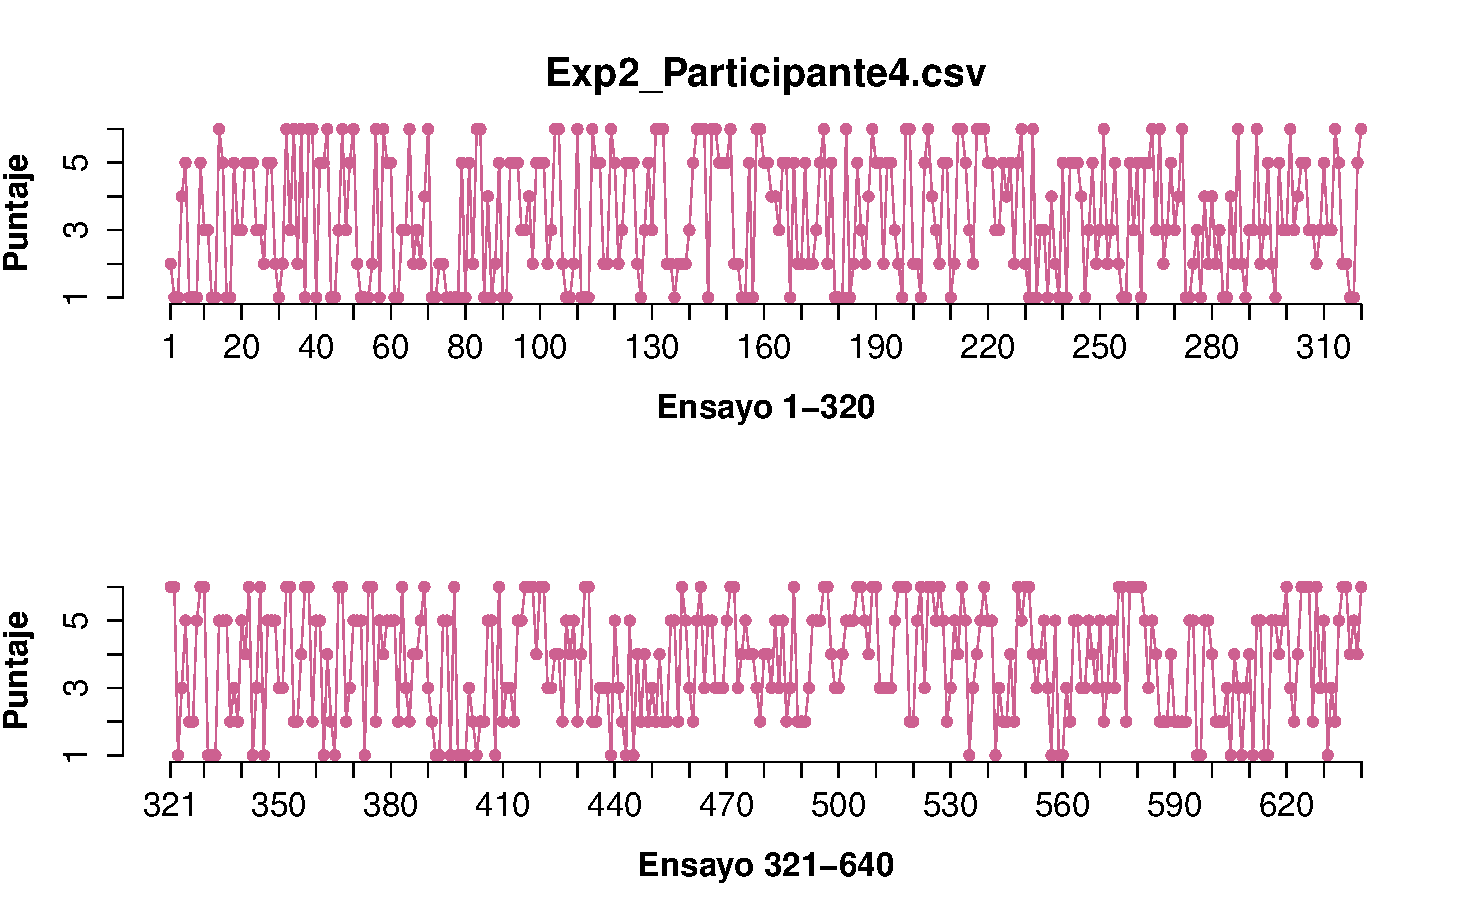
\includegraphics[width=0.30\textwidth]{Figures/Rating_Exp2_P4} 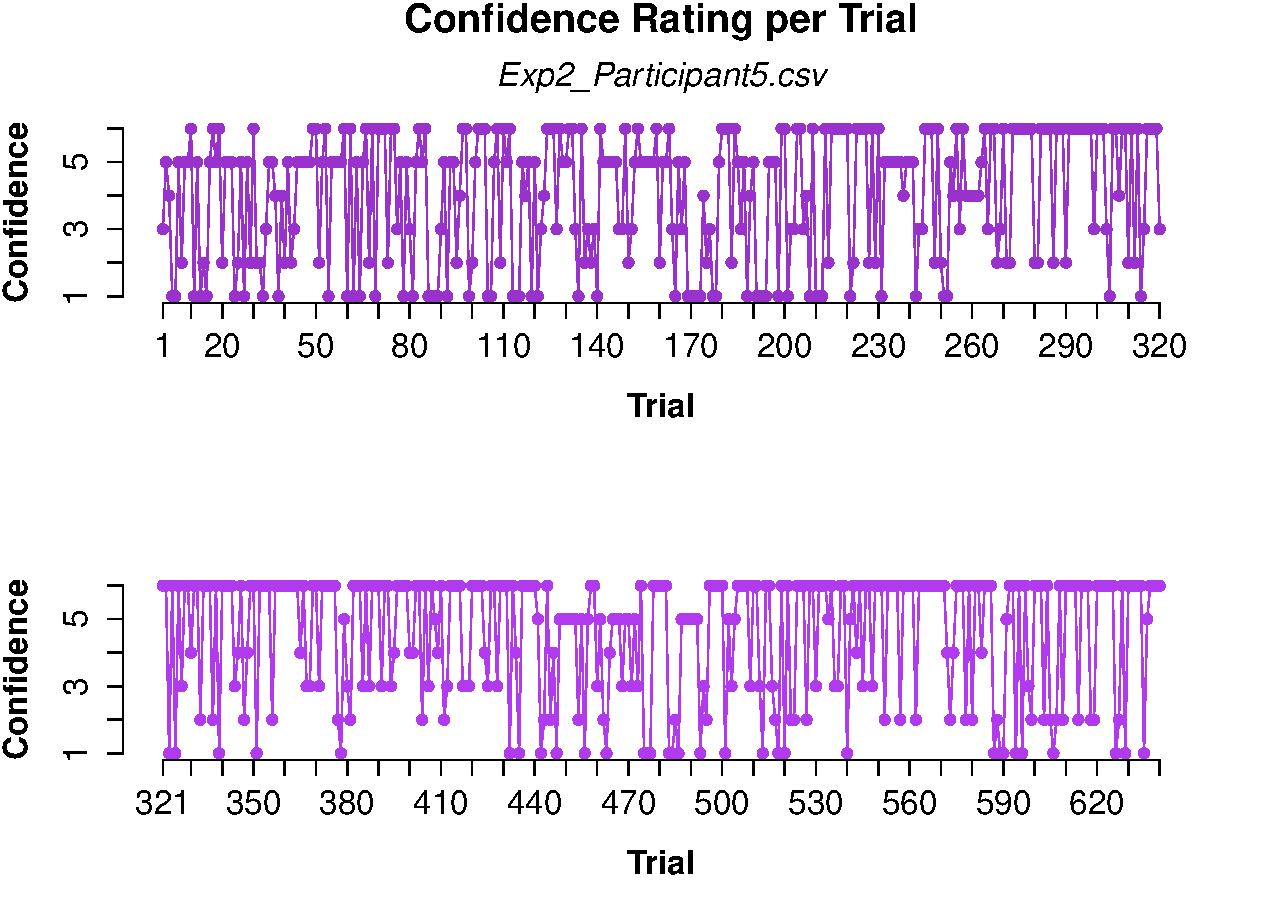
\includegraphics[width=0.30\textwidth]{Figures/Rating_Exp2_P5} 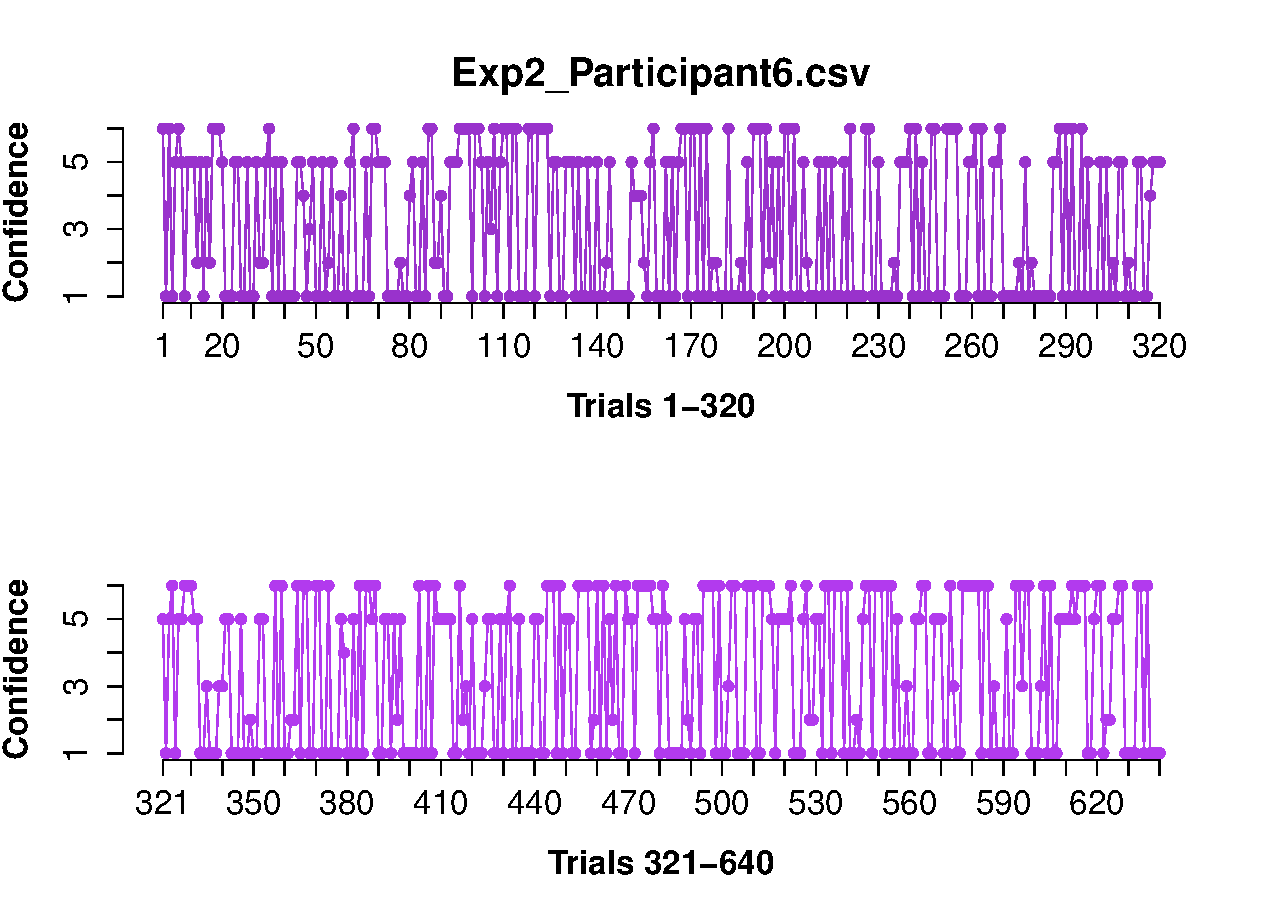
\includegraphics[width=0.30\textwidth]{Figures/Rating_Exp2_P6}
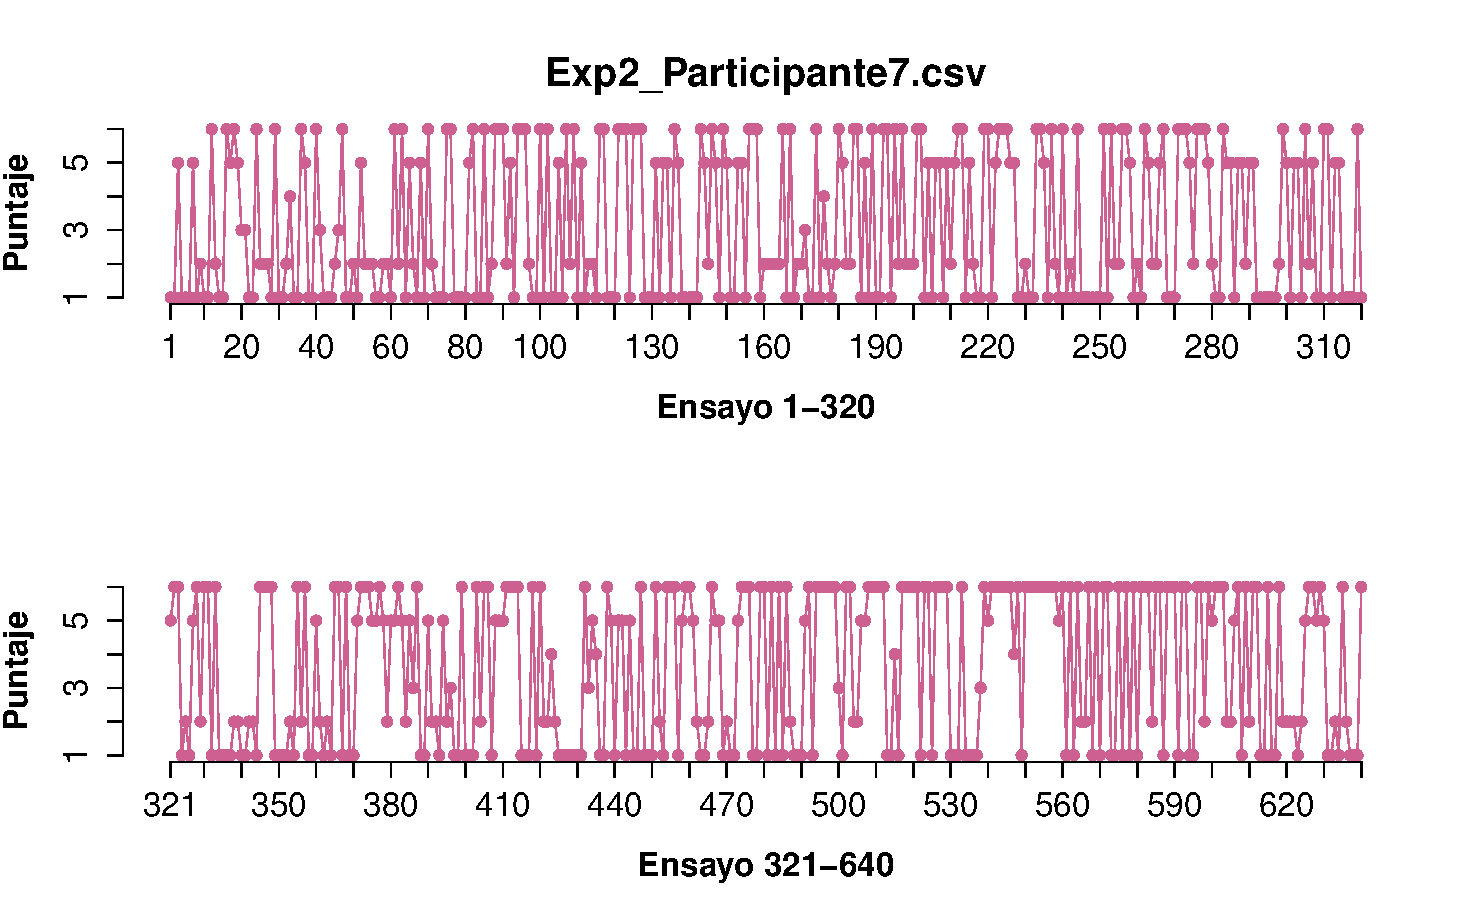
\includegraphics[width=0.30\textwidth]{Figures/Rating_Exp2_P7} 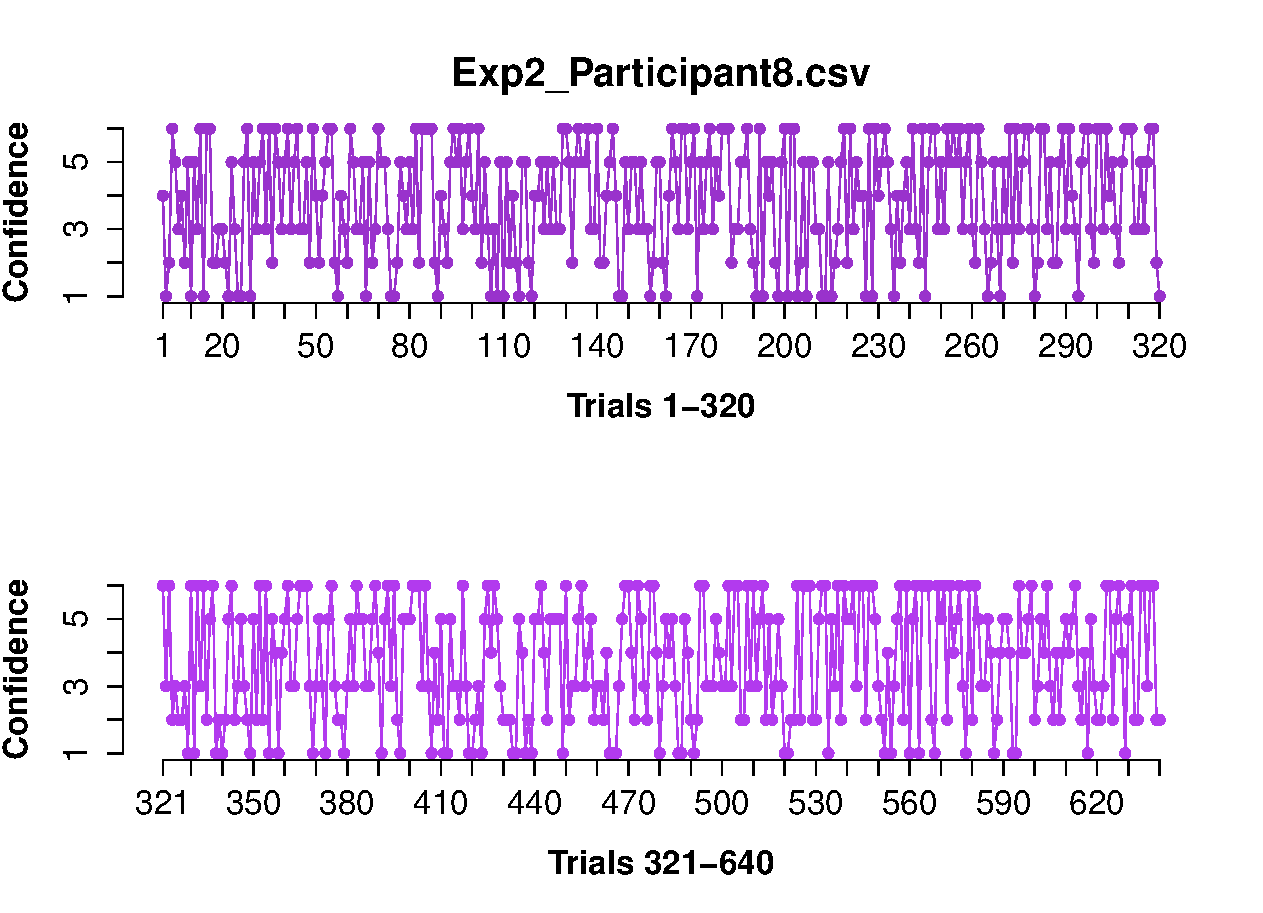
\includegraphics[width=0.30\textwidth]{Figures/Rating_Exp2_P8} 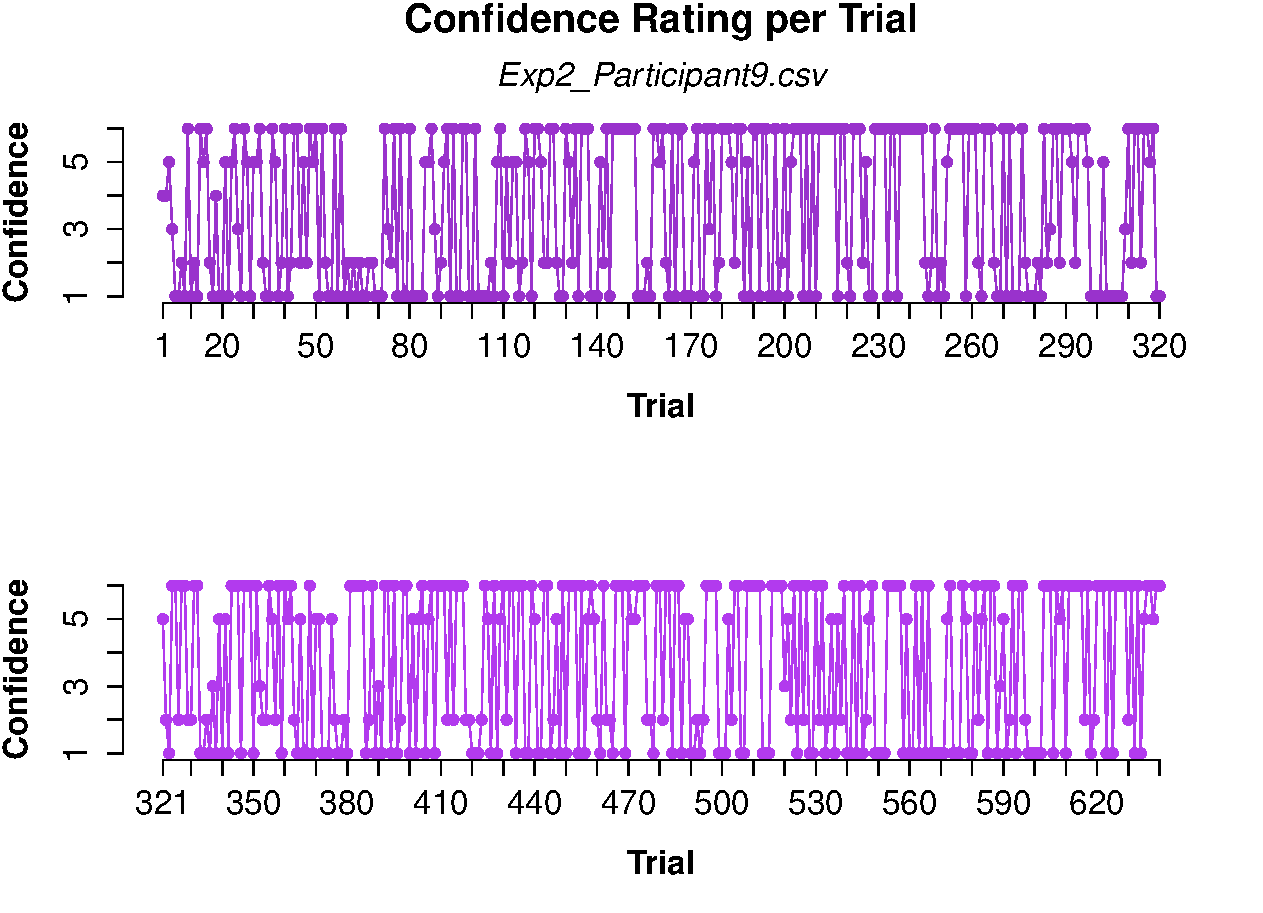
\includegraphics[width=0.30\textwidth]{Figures/Rating_Exp2_P9}
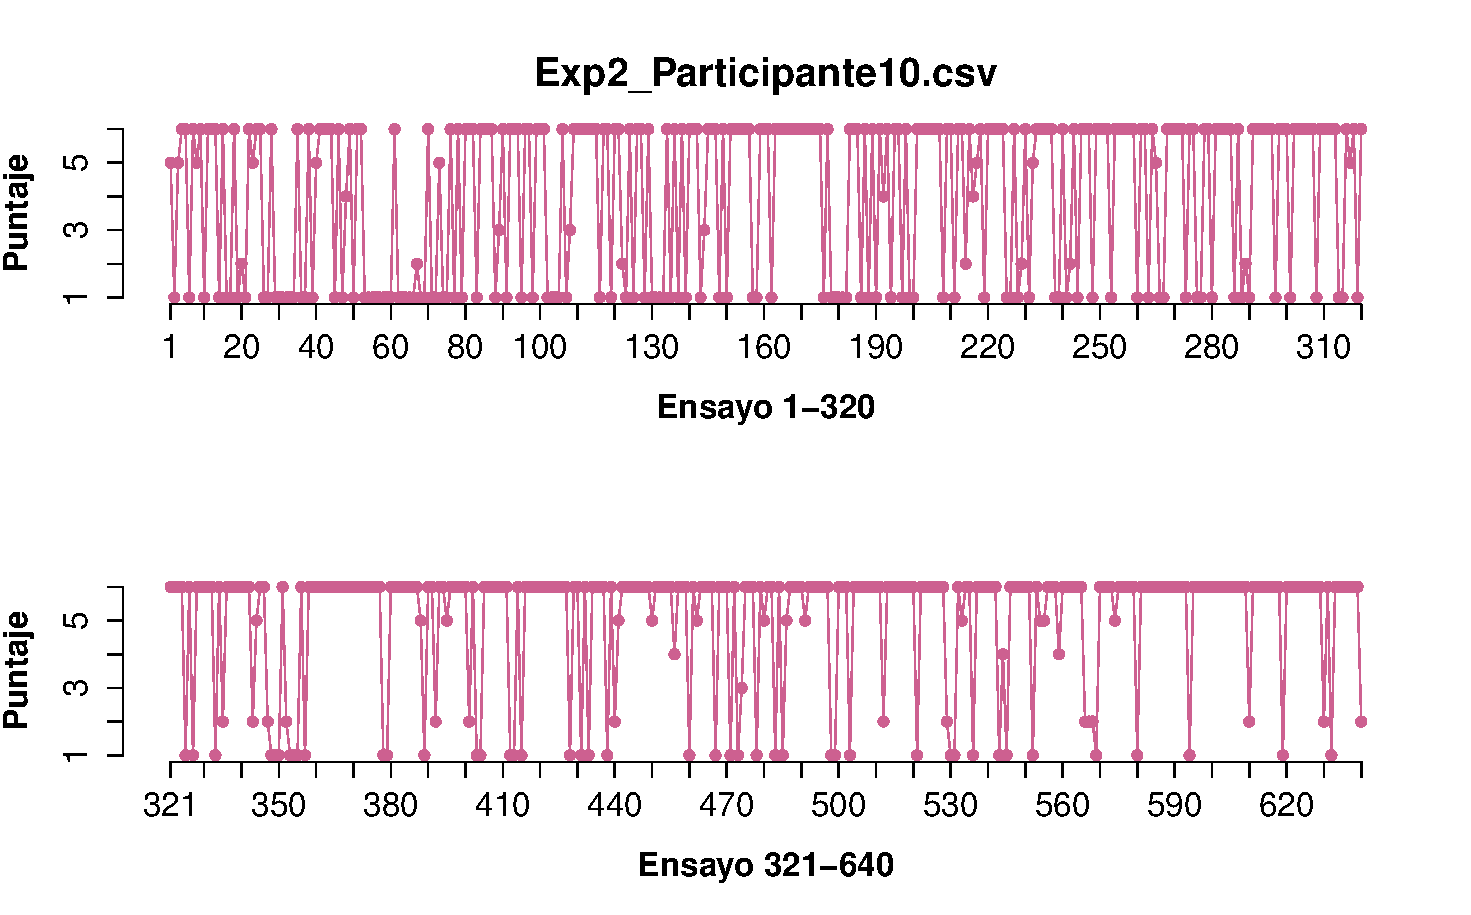
\includegraphics[width=0.30\textwidth]{Figures/Rating_Exp2_P10} 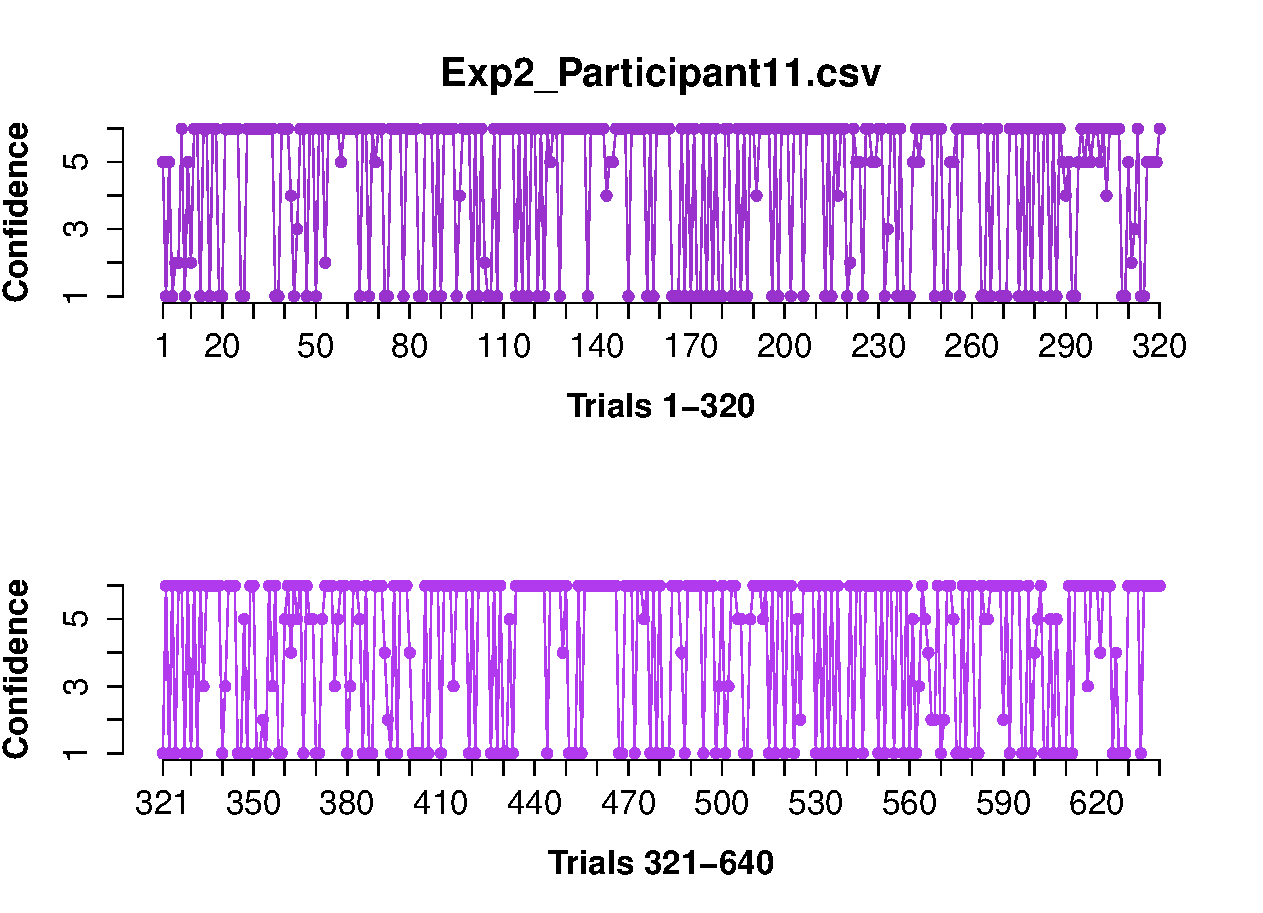
\includegraphics[width=0.30\textwidth]{Figures/Rating_Exp2_P11} 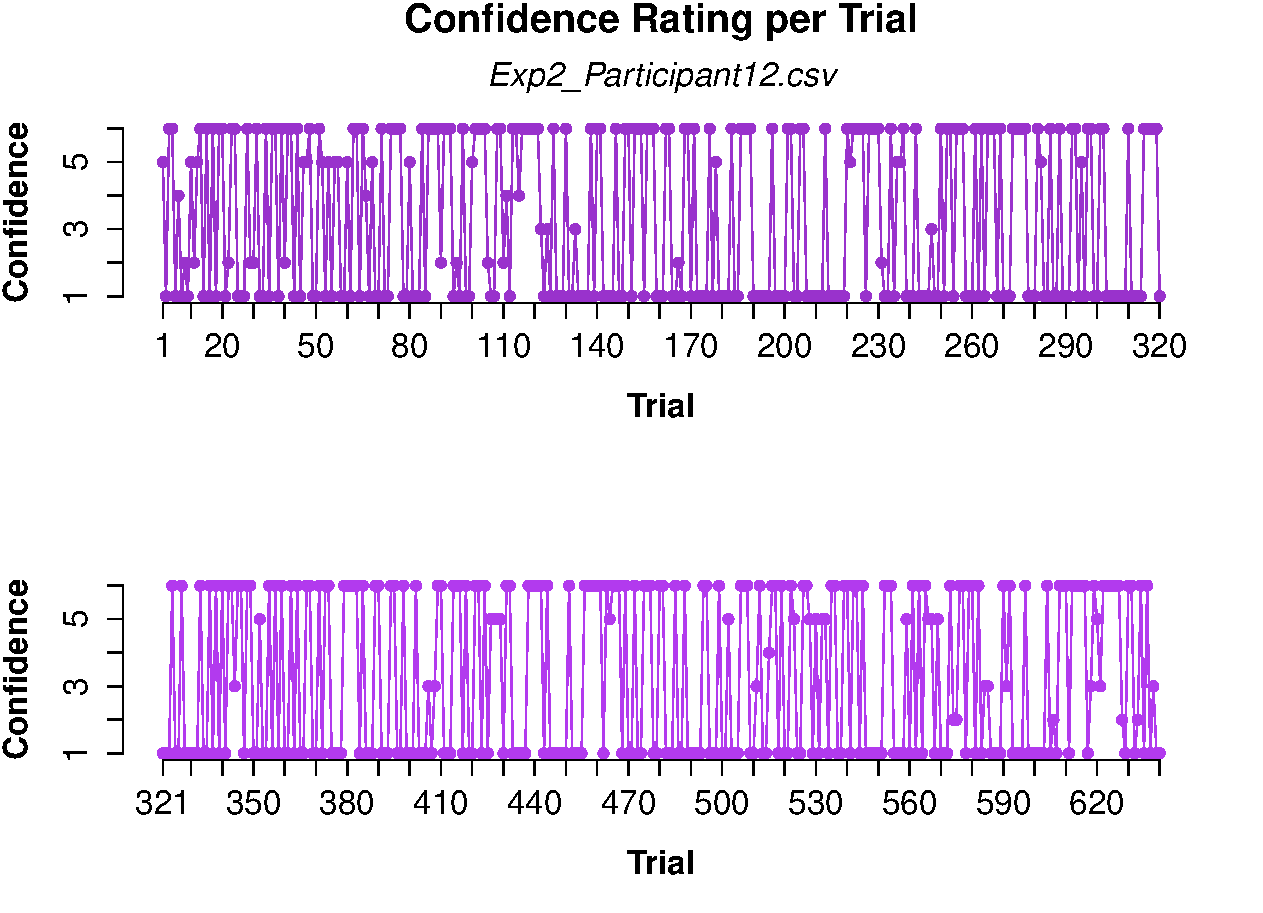
\includegraphics[width=0.30\textwidth]{Figures/Rating_Exp2_P12}
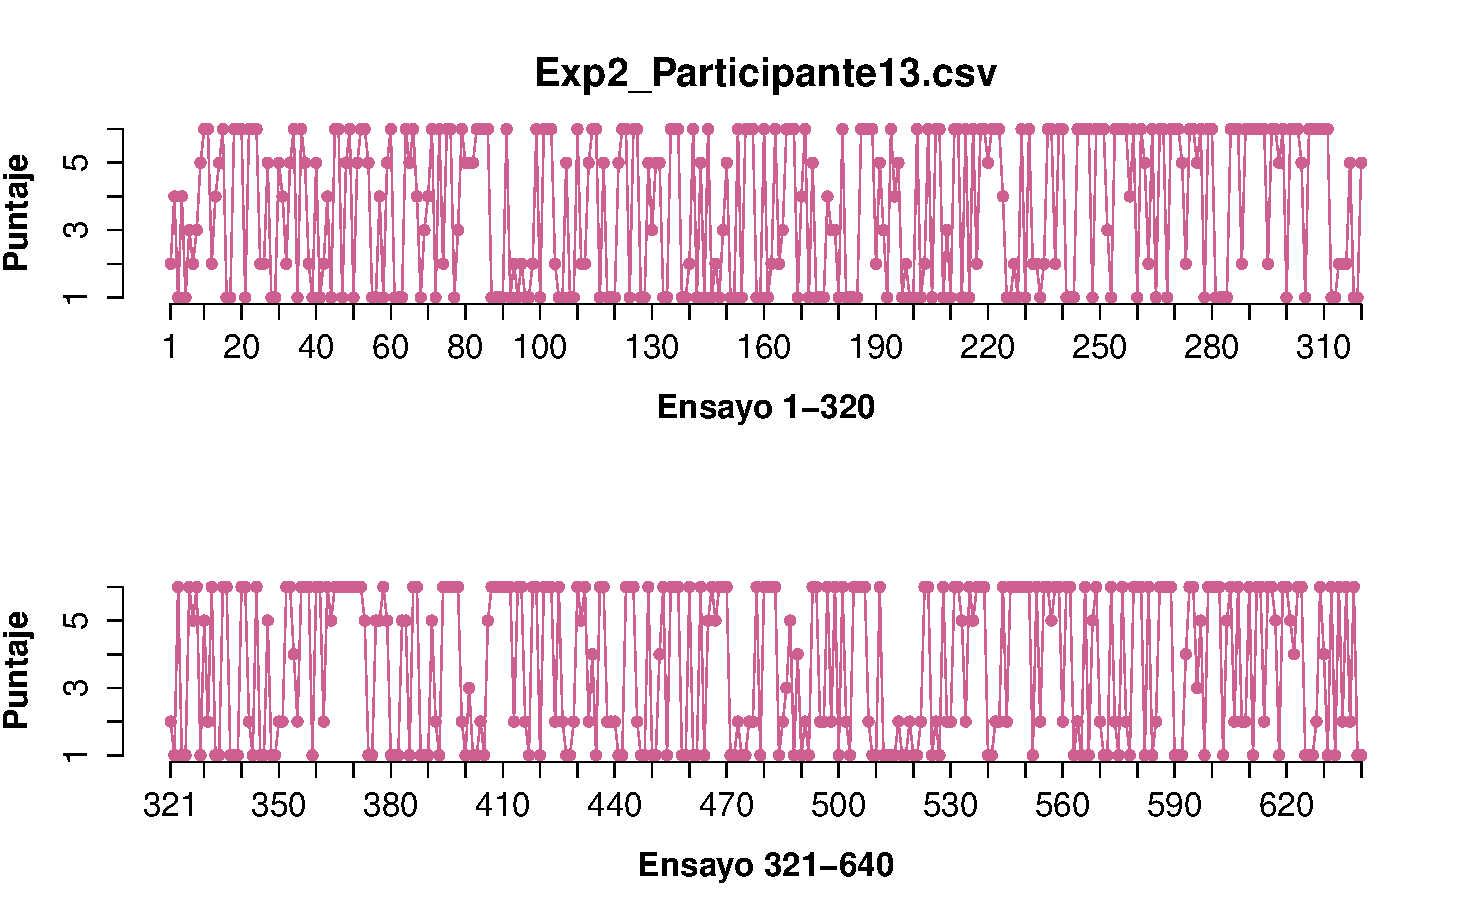
\includegraphics[width=0.30\textwidth]{Figures/Rating_Exp2_P13} 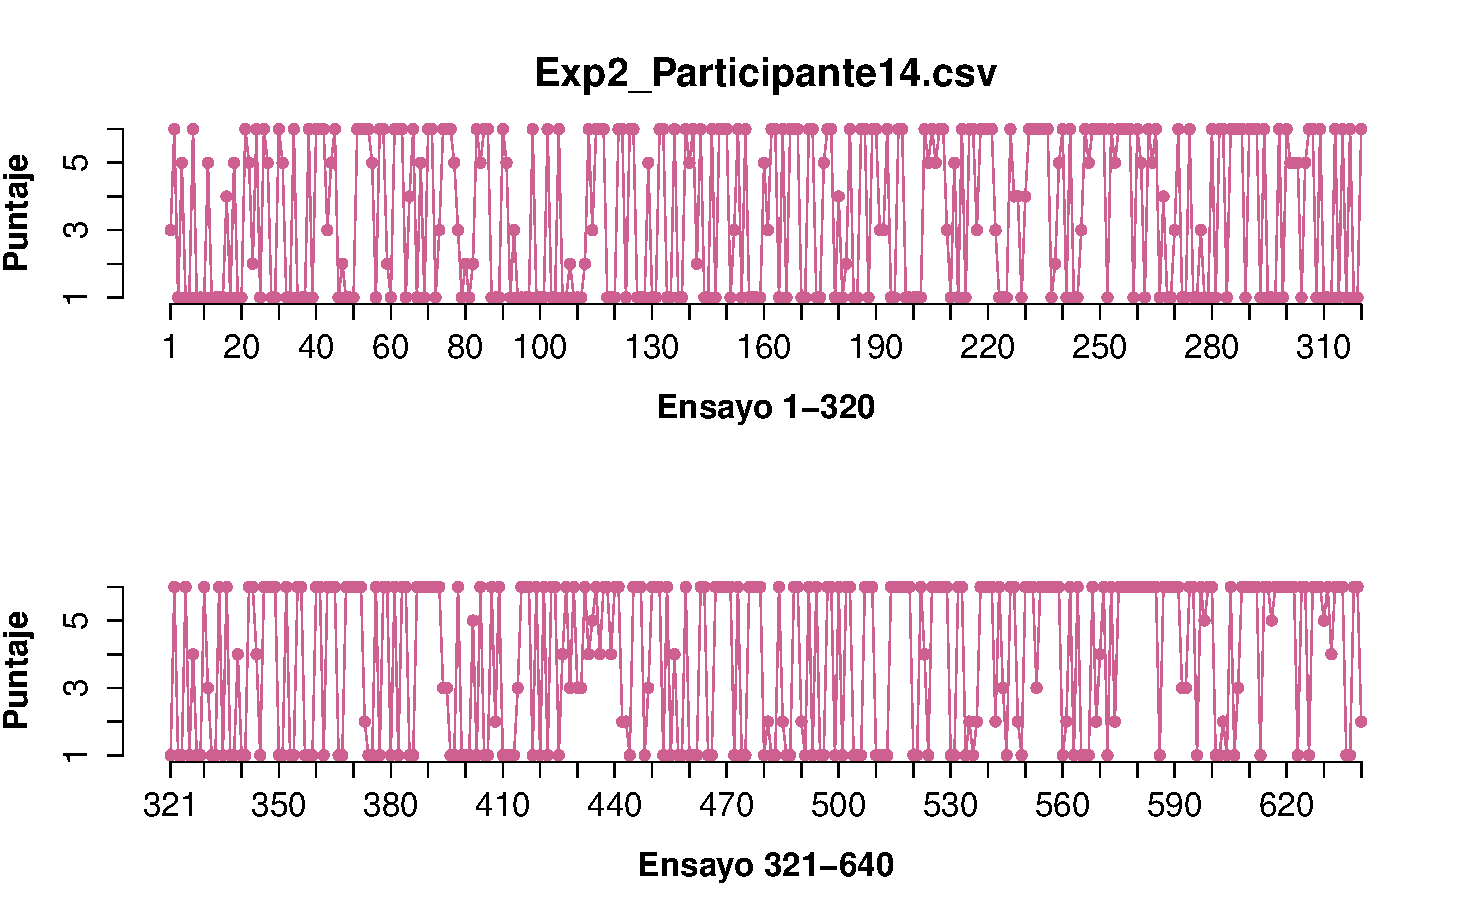
\includegraphics[width=0.30\textwidth]{Figures/Rating_Exp2_P14} 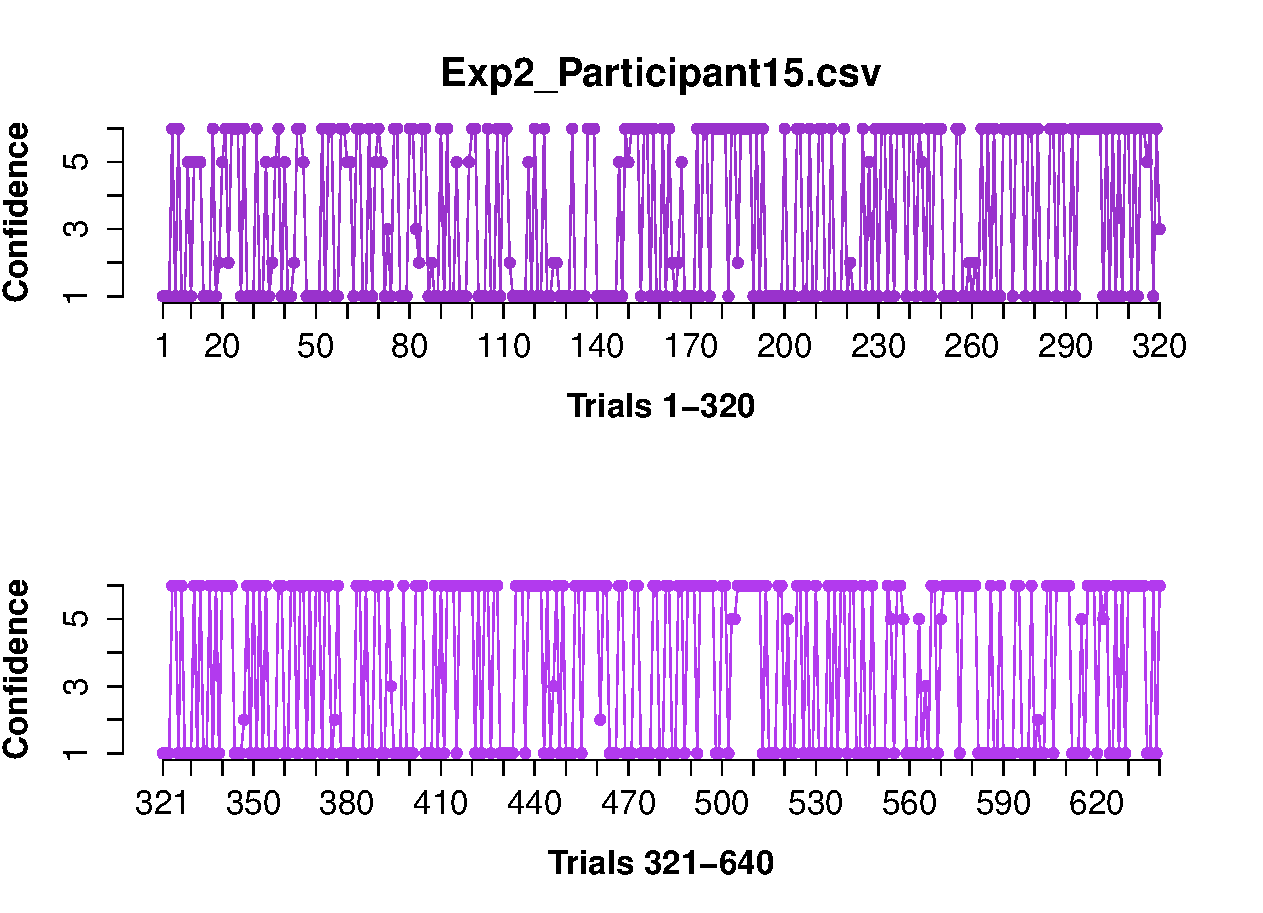
\includegraphics[width=0.30\textwidth]{Figures/Rating_Exp2_P15}
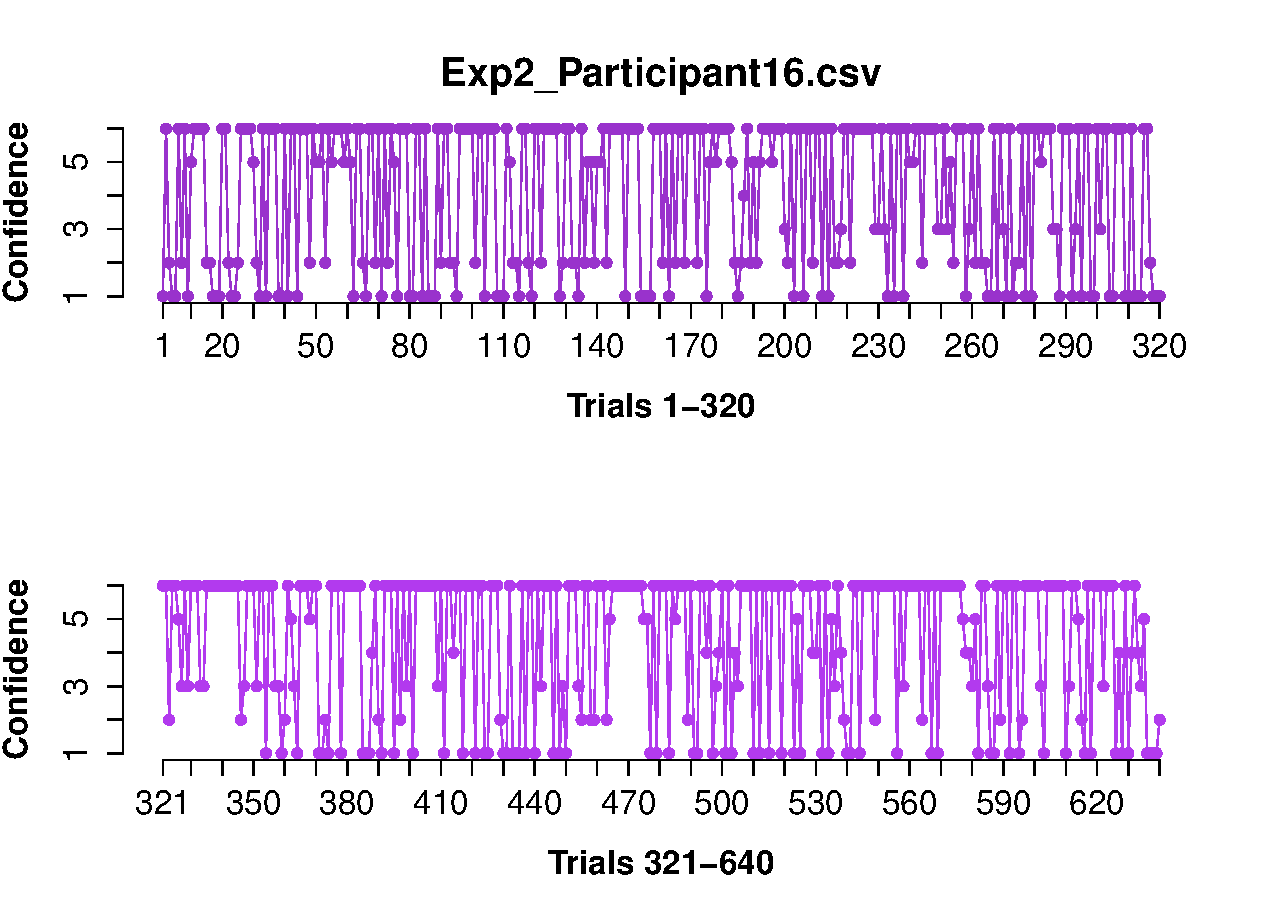
\includegraphics[width=0.30\textwidth]{Figures/Rating_Exp2_P16} 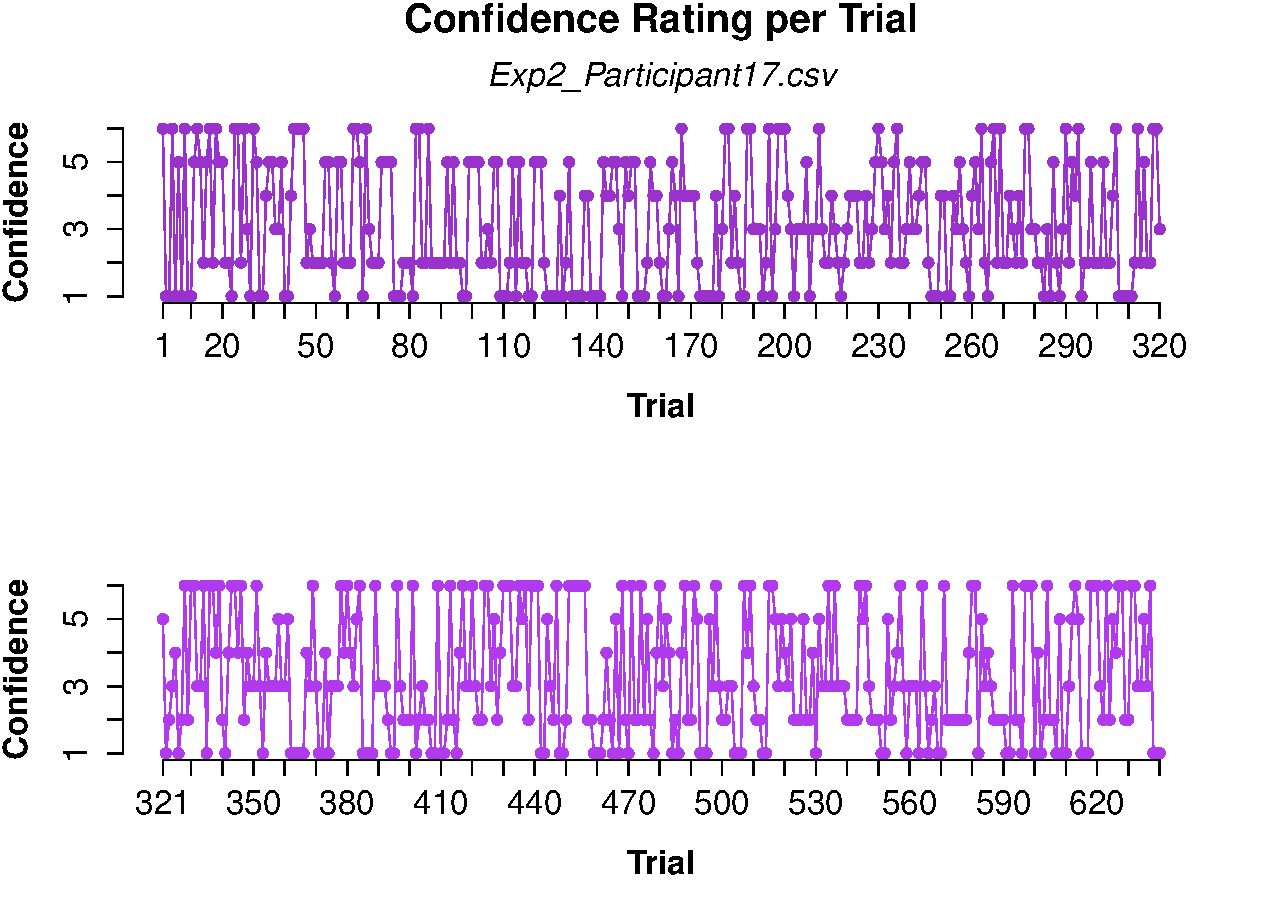
\includegraphics[width=0.30\textwidth]{Figures/Rating_Exp2_P17} 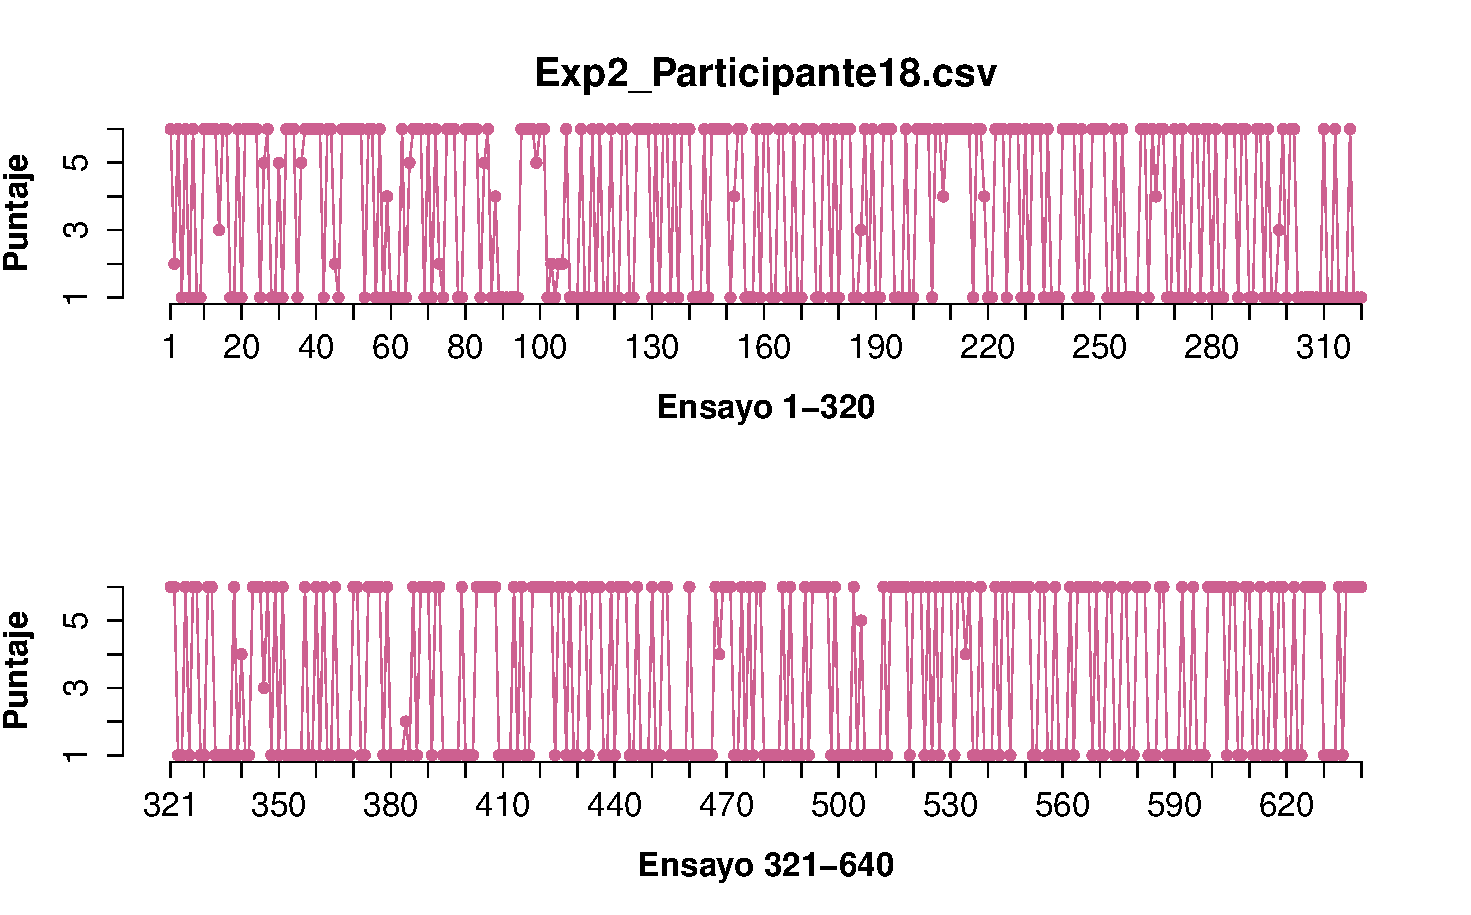
\includegraphics[width=0.30\textwidth]{Figures/Rating_Exp2_P18}
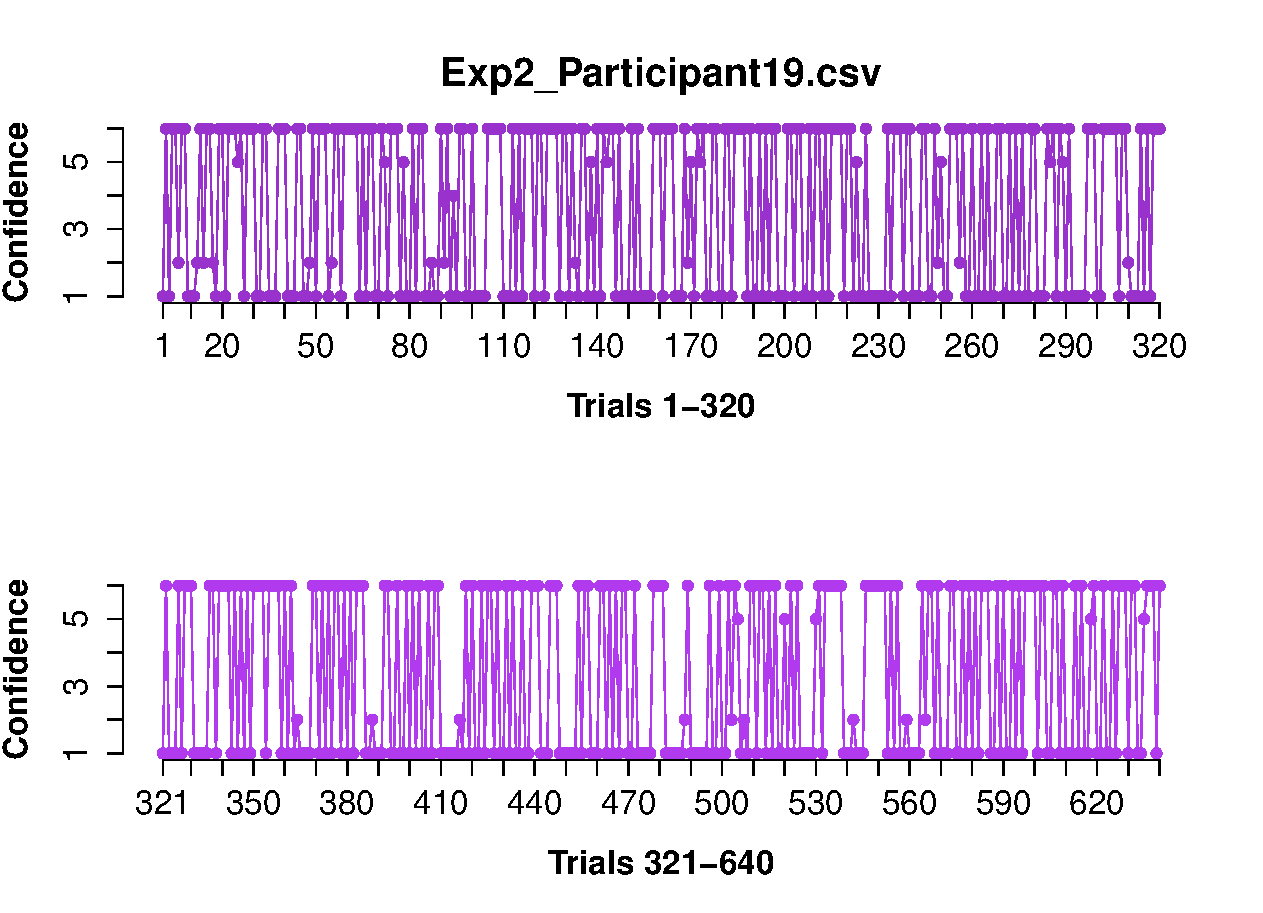
\includegraphics[width=0.30\textwidth]{Figures/Rating_Exp2_P19} 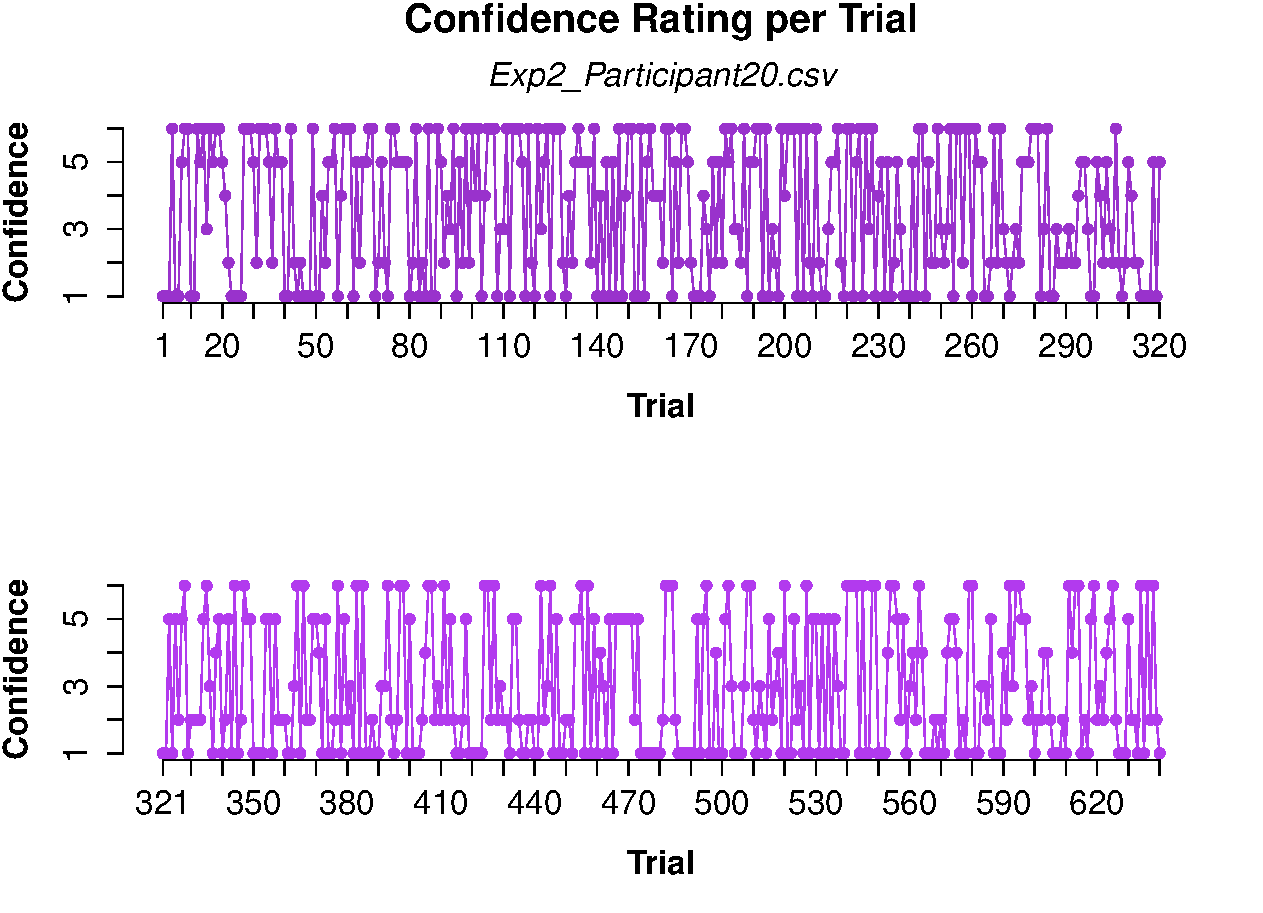
\includegraphics[width=0.30\textwidth]{Figures/Rating_Exp2_P20} 
%\decoRule
\caption[Rating_Exp2]{Puntaje asignado a a Escala por ensayo (Experimento 2).}
\label{fig:Rating_E2}
\end{figure}




\subsection{Control 2: Evaluando tiempos de respuesta a lo largo del experimento}


%%%%%%%%%%%%%%%%%%%%%%%%%%%%%%%%%%%%%%%%%%%%%%%%%%%%%%%%%%%%%%
%%%%%%%%%  Respuesta Rating en los ensayos
% Experimento 2
%%%%%%%%%%%%%%%%%%%%%%%%%%%%%%%%%%%%%%%%%%%%%%%%%%%%%%%%%%%%%%%
\begin{figure}[th]
\centering
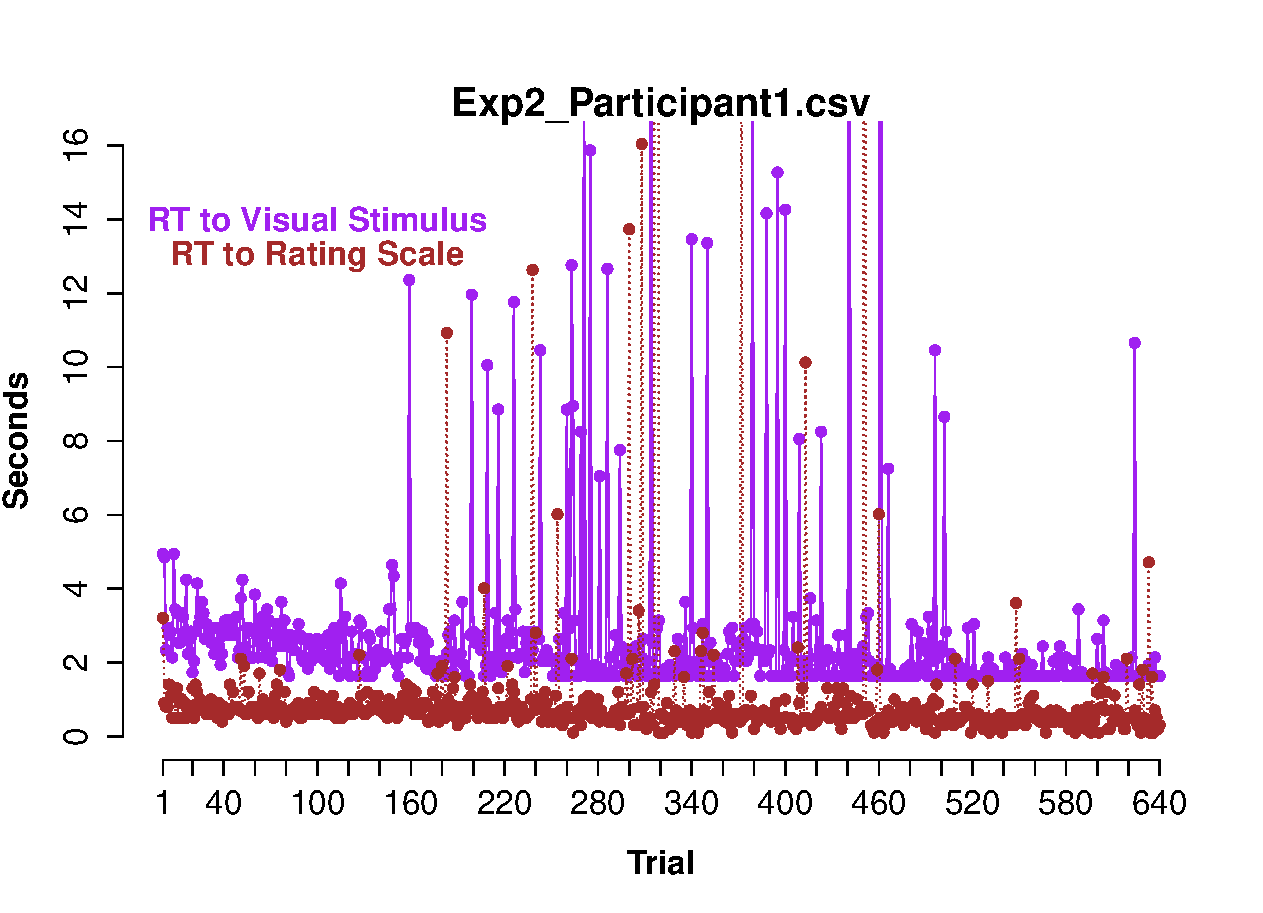
\includegraphics[width=0.30\textwidth]{Figures/RTs_Exp2_P1} 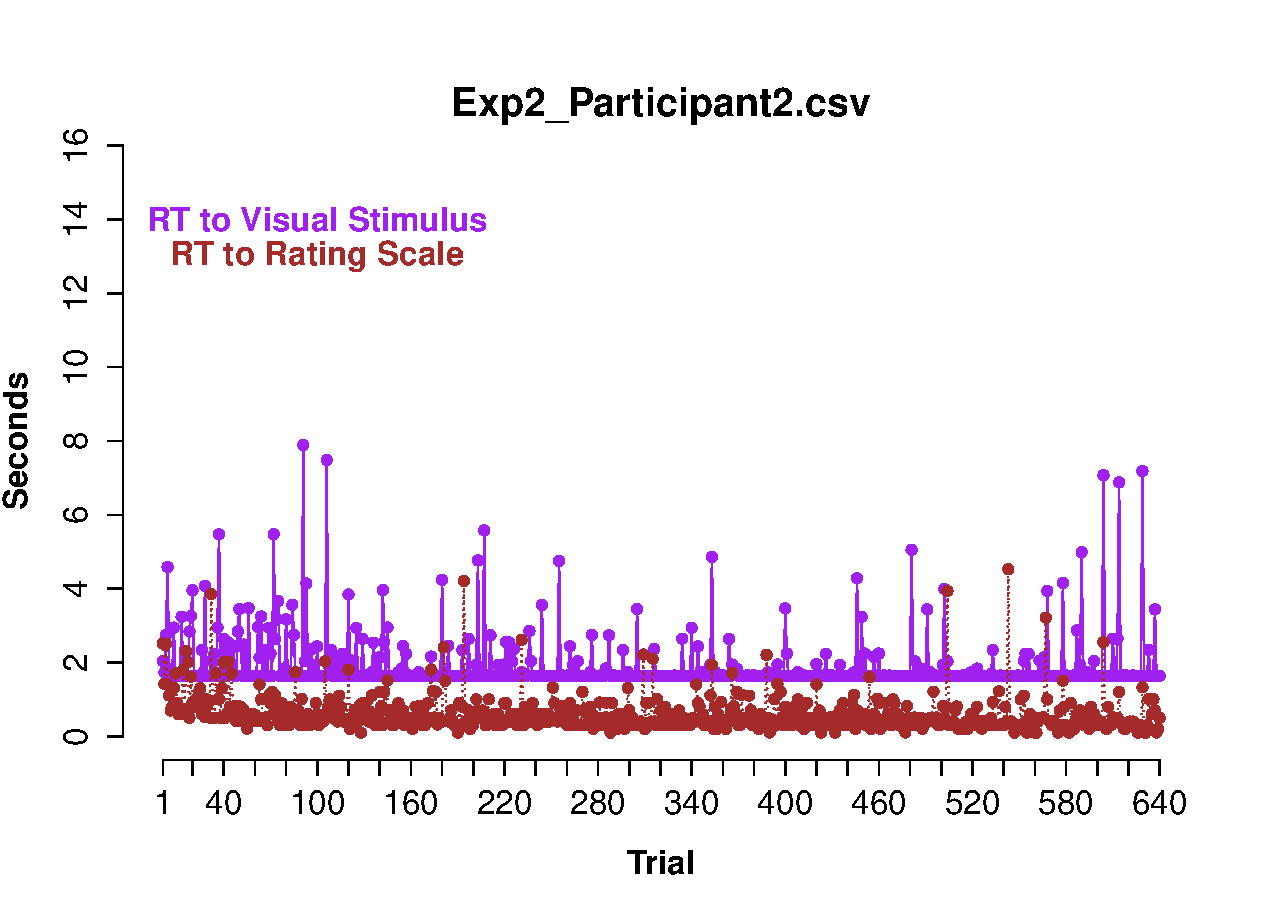
\includegraphics[width=0.30\textwidth]{Figures/RTs_Exp2_P2} 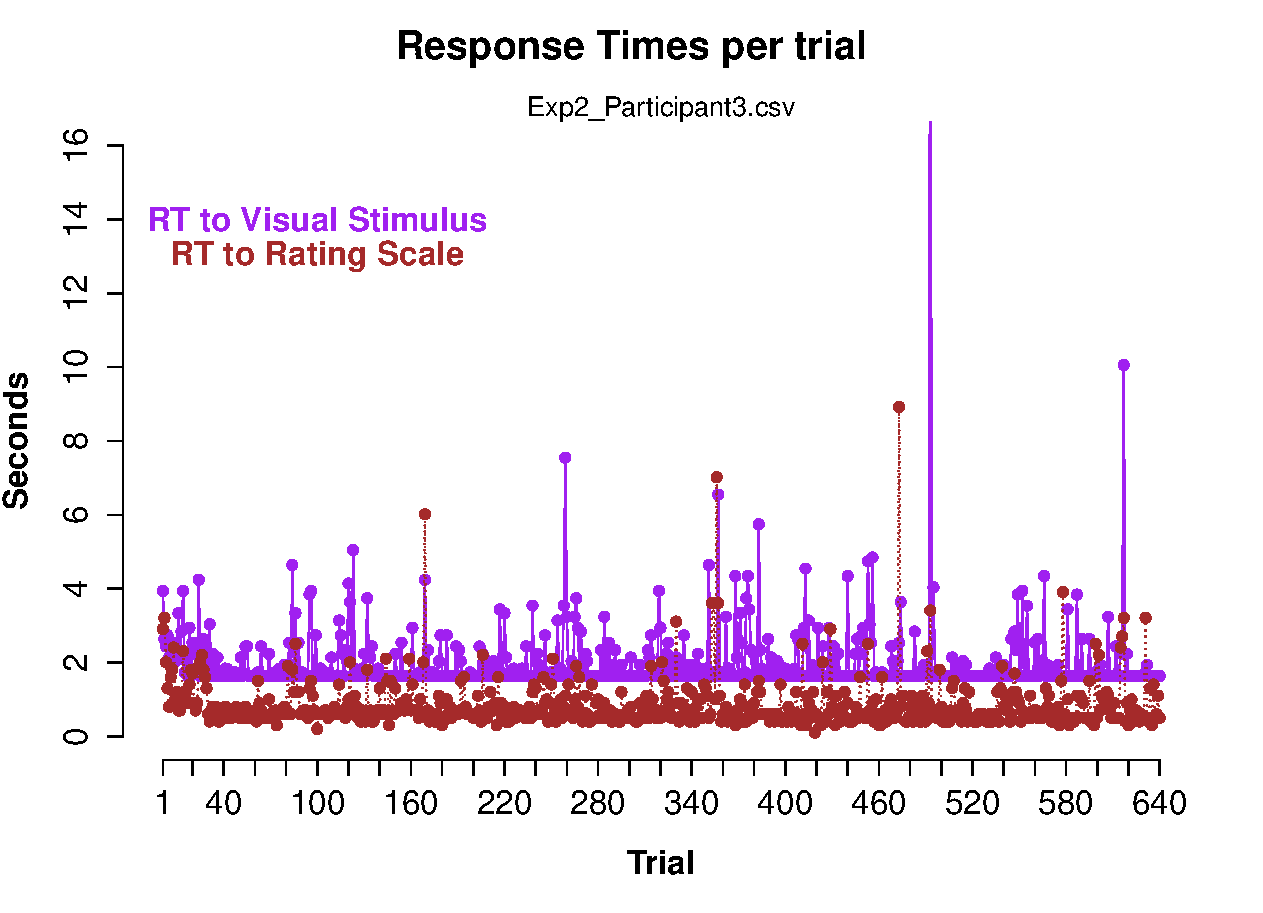
\includegraphics[width=0.30\textwidth]{Figures/RTs_Exp2_P3}
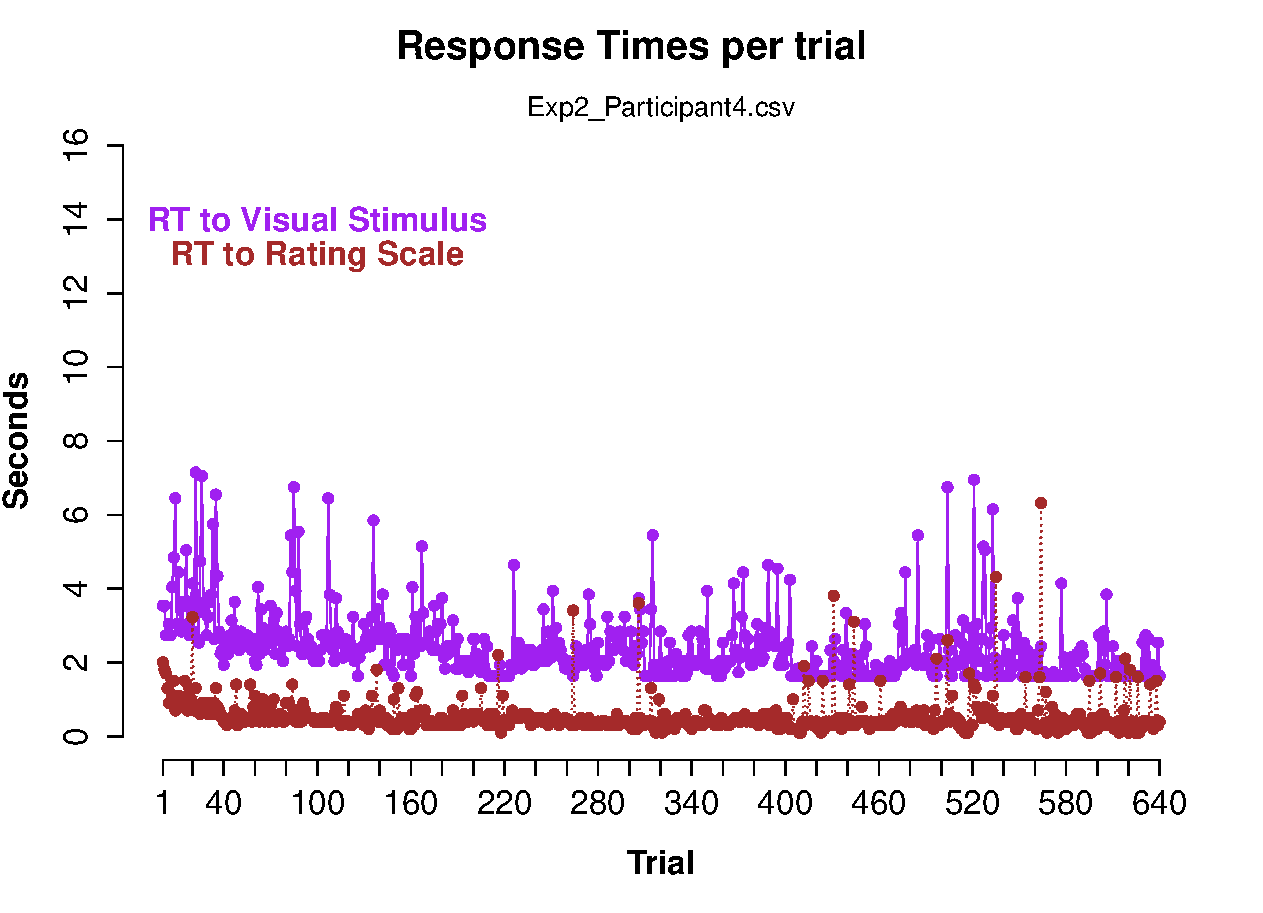
\includegraphics[width=0.30\textwidth]{Figures/RTs_Exp2_P4} 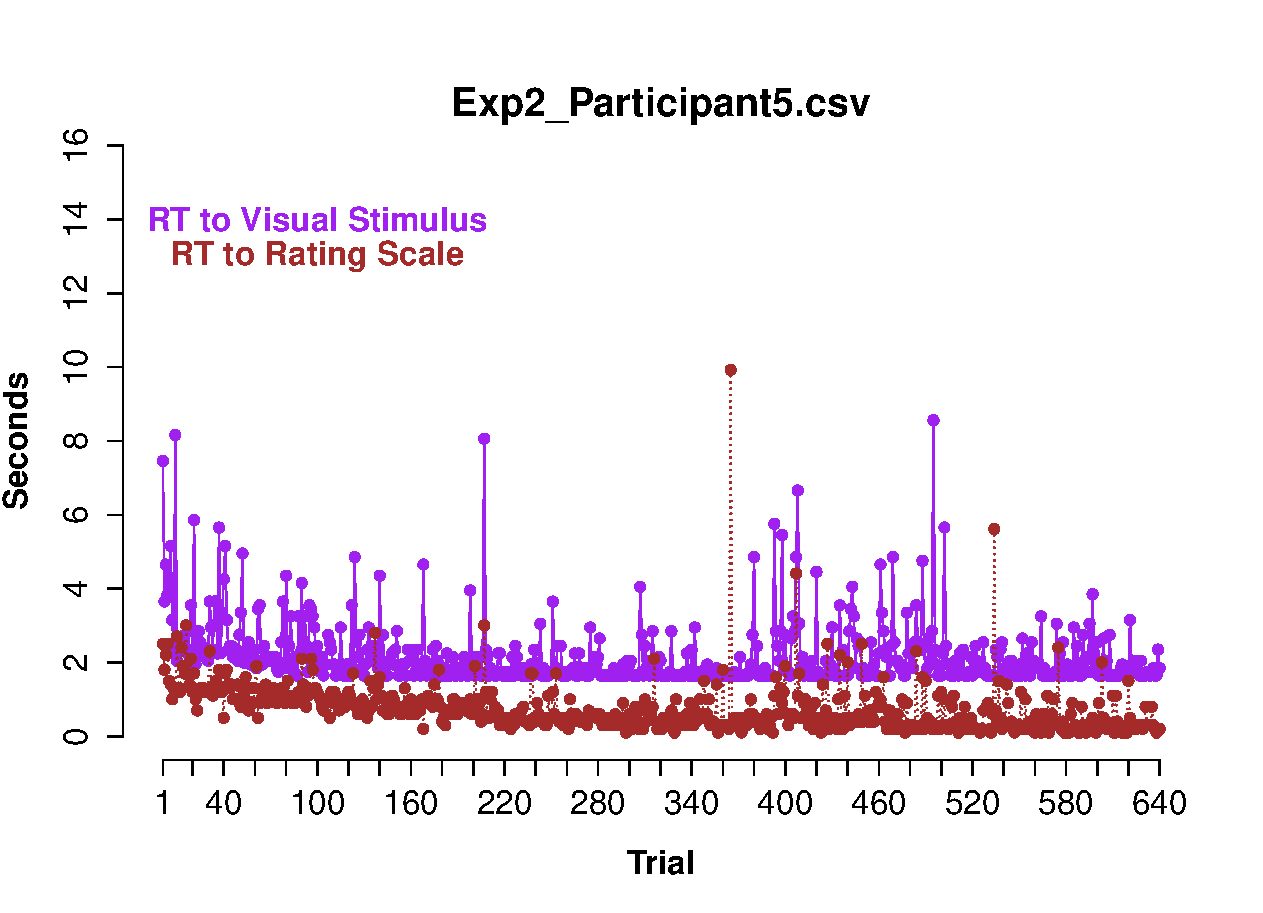
\includegraphics[width=0.30\textwidth]{Figures/RTs_Exp2_P5} 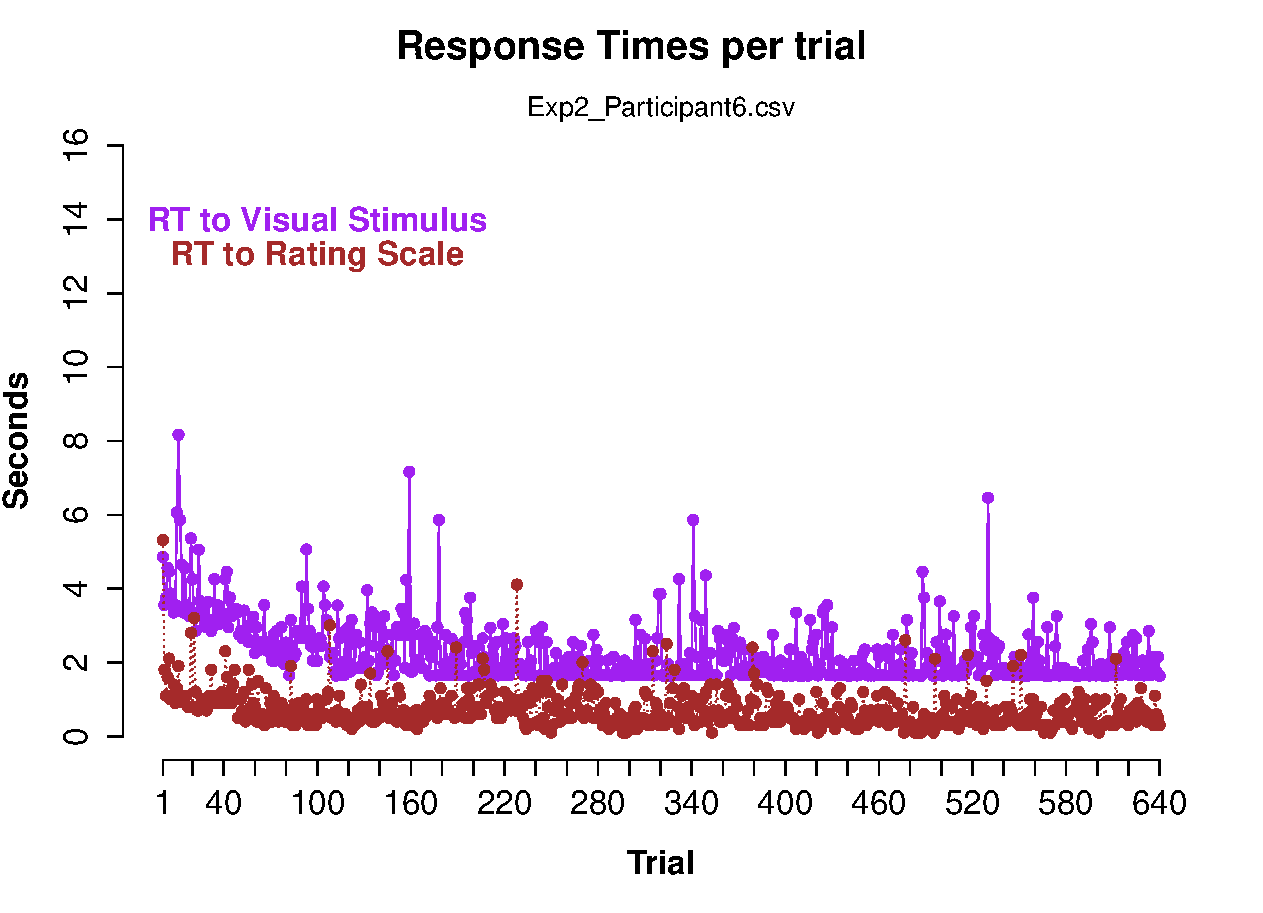
\includegraphics[width=0.30\textwidth]{Figures/RTs_Exp2_P6}
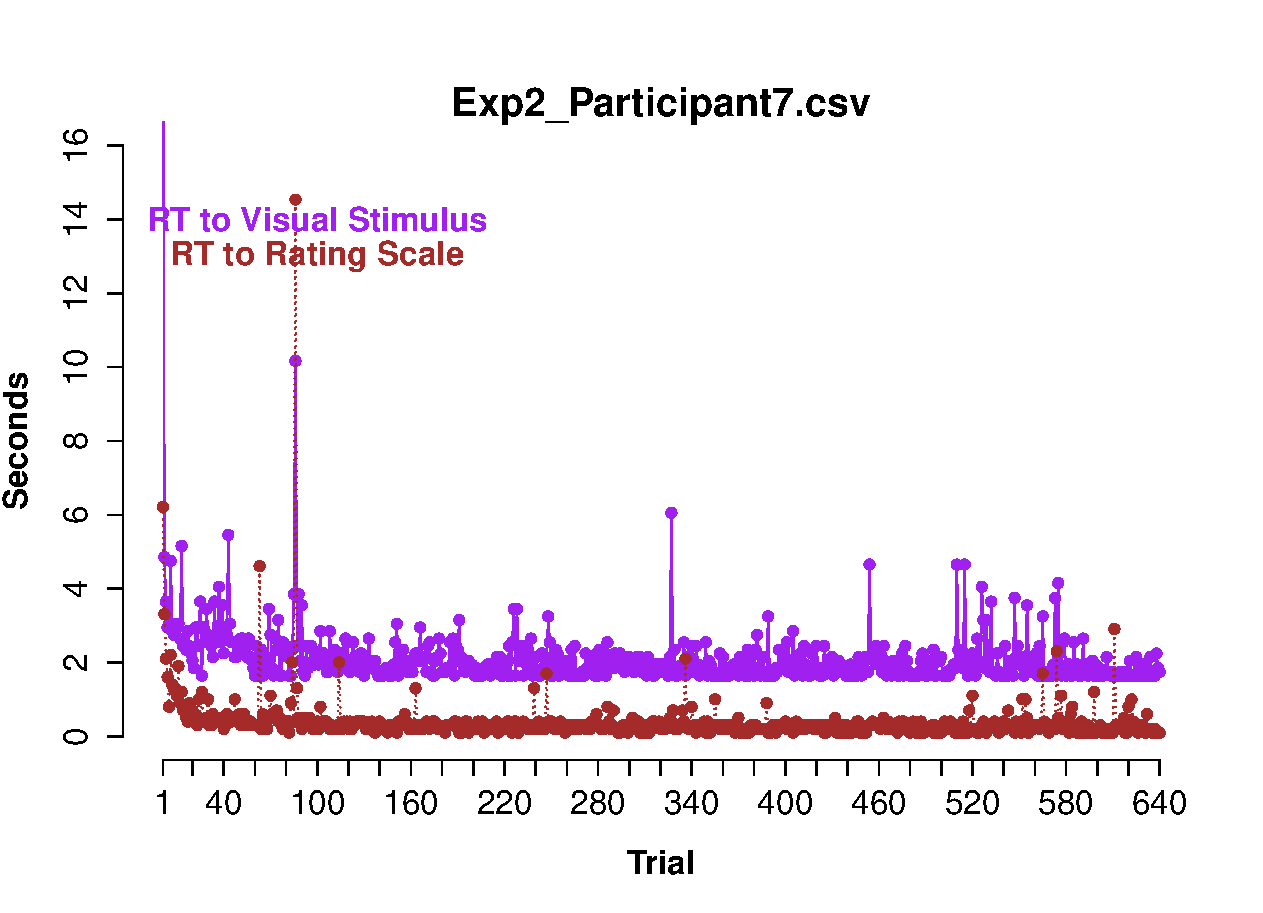
\includegraphics[width=0.30\textwidth]{Figures/RTs_Exp2_P7} \includegraphics[width=0.30\textwidth]{Figures/RTs_Exp2_P8} \includegraphics[width=0.30\textwidth]{Figures/RTs_Exp2_P9}
\includegraphics[width=0.30\textwidth]{Figures/RTs_Exp2_P10} \includegraphics[width=0.30\textwidth]{Figures/RTs_Exp2_P11} \includegraphics[width=0.30\textwidth]{Figures/RTs_Exp2_P12}
\includegraphics[width=0.30\textwidth]{Figures/RTs_Exp2_P13} \includegraphics[width=0.30\textwidth]{Figures/RTs_Exp2_P14} \includegraphics[width=0.30\textwidth]{Figures/RTs_Exp2_P15}
\includegraphics[width=0.30\textwidth]{Figures/RTs_Exp2_P16} \includegraphics[width=0.30\textwidth]{Figures/RTs_Exp2_P17} \includegraphics[width=0.30\textwidth]{Figures/RTs_Exp2_P18}
\includegraphics[width=0.30\textwidth]{Figures/RTs_Exp2_P19} \includegraphics[width=0.30\textwidth]{Figures/RTs_Exp2_P20} 
%\decoRule
\caption[Rating_Exp2]{Tiempos de Respuesta por ensayo (Experimento 2).}
\label{fig:Rating_E2}
\end{figure}


%%%%%%%%%%%%%%%%%%%%%%%%%%%%%%%%%%%%%%%%%%%%%%%%%%%%%%%%%%%%%%
%%%%%%%%%  Respuesta Rating en los ensayos
% Experimento 2
%%%%%%%%%%%%%%%%%%%%%%%%%%%%%%%%%%%%%%%%%%%%%%%%%%%%%%%%%%%%%%%
\begin{figure}[th]
\centering
\includegraphics[width=0.30\textwidth]{Figures/RT1_Exp2_P1} \includegraphics[width=0.30\textwidth]{Figures/RT1_Exp2_P2} \includegraphics[width=0.30\textwidth]{Figures/RT1_Exp2_P3}
\includegraphics[width=0.30\textwidth]{Figures/RT1_Exp2_P4} \includegraphics[width=0.30\textwidth]{Figures/RT1_Exp2_P5} \includegraphics[width=0.30\textwidth]{Figures/RT1_Exp2_P6}
\includegraphics[width=0.30\textwidth]{Figures/RT1_Exp2_P7} \includegraphics[width=0.30\textwidth]{Figures/RT1_Exp2_P8} \includegraphics[width=0.30\textwidth]{Figures/RT1_Exp2_P9}
\includegraphics[width=0.30\textwidth]{Figures/RT1_Exp2_P10} \includegraphics[width=0.30\textwidth]{Figures/RT1_Exp2_P11} \includegraphics[width=0.30\textwidth]{Figures/RT1_Exp2_P12}
\includegraphics[width=0.30\textwidth]{Figures/RT1_Exp2_P13} \includegraphics[width=0.30\textwidth]{Figures/RT1_Exp2_P14} \includegraphics[width=0.30\textwidth]{Figures/RT1_Exp2_P15}
\includegraphics[width=0.30\textwidth]{Figures/RT1_Exp2_P16} \includegraphics[width=0.30\textwidth]{Figures/RT1_Exp2_P17} \includegraphics[width=0.30\textwidth]{Figures/RT1_Exp2_P18}
\includegraphics[width=0.30\textwidth]{Figures/RT1_Exp2_P19} \includegraphics[width=0.30\textwidth]{Figures/RT1_Exp2_P20} 
%\decoRule
\caption[Rating_Exp2]{Tiempo de Respuesta a la tarea perceptual por ensayo (Experimento 2).}
\label{fig:Rating_E2}
\end{figure}


%%%%%%%%%%%%%%%%%%%%%%%%%%%%%%%%%%%%%%%%%%%%%%%%%%%%%%%%%%%%%%
%%%%%%%%%  Respuesta Rating en los ensayos
% Experimento 2
%%%%%%%%%%%%%%%%%%%%%%%%%%%%%%%%%%%%%%%%%%%%%%%%%%%%%%%%%%%%%%%
\begin{figure}[th]
\centering
\includegraphics[width=0.30\textwidth]{Figures/RT2_Exp2_P1} \includegraphics[width=0.30\textwidth]{Figures/RT2_Exp2_P2} \includegraphics[width=0.30\textwidth]{Figures/RT2_Exp2_P3}
\includegraphics[width=0.30\textwidth]{Figures/RT2_Exp2_P4} \includegraphics[width=0.30\textwidth]{Figures/RT2_Exp2_P5} \includegraphics[width=0.30\textwidth]{Figures/RT2_Exp2_P6}
\includegraphics[width=0.30\textwidth]{Figures/RT2_Exp2_P7} \includegraphics[width=0.30\textwidth]{Figures/RT2_Exp2_P8} \includegraphics[width=0.30\textwidth]{Figures/RT2_Exp2_P9}
\includegraphics[width=0.30\textwidth]{Figures/RT2_Exp2_P10} \includegraphics[width=0.30\textwidth]{Figures/RT2_Exp2_P11} \includegraphics[width=0.30\textwidth]{Figures/RT2_Exp2_P12}
\includegraphics[width=0.30\textwidth]{Figures/RT2_Exp2_P13} \includegraphics[width=0.30\textwidth]{Figures/RT2_Exp2_P14} \includegraphics[width=0.30\textwidth]{Figures/RT2_Exp2_P15}
\includegraphics[width=0.30\textwidth]{Figures/RT2_Exp2_P16} \includegraphics[width=0.30\textwidth]{Figures/RT2_Exp2_P17} \includegraphics[width=0.30\textwidth]{Figures/RT2_Exp2_P18}
\includegraphics[width=0.30\textwidth]{Figures/RT2_Exp2_P19} \includegraphics[width=0.30\textwidth]{Figures/RT2_Exp2_P20} 
%\decoRule
\caption[Rating_Exp2]{Tiempo de respuesta a la escala de confianza por ensayo (Experimento 2).}
\label{fig:Rating_E2}
\end{figure}



\subsection{Control 3: ¿La duración del experimento tuvo un impacto en la ejecución de los participantes?}


%%%%%%%%%%%%%%%%%%%%%%%%%%%%%%%%%%%%%%%%%%%%%%%%%%%%%%%%%%%%%%
%%%%%%%%%  Respuesta (Y/N) en los ensayos
% Experimento 2
%%%%%%%%%%%%%%%%%%%%%%%%%%%%%%%%%%%%%%%%%%%%%%%%%%%%%%%%%%%%%%%
\begin{figure}[th]
\centering
\includegraphics[width=0.30\textwidth]{Figures/Success_Exp1_P1} \includegraphics[width=0.30\textwidth]{Figures/Success_Exp1_P2} \includegraphics[width=0.30\textwidth]{Figures/Success_Exp1_P3}
\includegraphics[width=0.30\textwidth]{Figures/Success_Exp1_P4} \includegraphics[width=0.30\textwidth]{Figures/Success_Exp1_P5} \includegraphics[width=0.30\textwidth]{Figures/Success_Exp1_P6}
\includegraphics[width=0.30\textwidth]{Figures/Success_Exp1_P7} \includegraphics[width=0.30\textwidth]{Figures/Success_Exp1_P8} \includegraphics[width=0.30\textwidth]{Figures/Success_Exp1_P9}
\includegraphics[width=0.30\textwidth]{Figures/Success_Exp1_P10} \includegraphics[width=0.30\textwidth]{Figures/Success_Exp1_P11} \includegraphics[width=0.30\textwidth]{Figures/Success_Exp1_P12}
\includegraphics[width=0.30\textwidth]{Figures/Success_Exp1_P13} \includegraphics[width=0.30\textwidth]{Figures/Success_Exp1_P14} \includegraphics[width=0.30\textwidth]{Figures/Success_Exp1_P15}
\includegraphics[width=0.30\textwidth]{Figures/Success_Exp1_P16} \includegraphics[width=0.30\textwidth]{Figures/Success_Exp1_P17} \includegraphics[width=0.30\textwidth]{Figures/Success_Exp1_P18}
\includegraphics[width=0.30\textwidth]{Figures/Success_Exp1_P19} \includegraphics[width=0.30\textwidth]{Figures/Success_Exp1_P20} \includegraphics[width=0.30\textwidth]{Figures/Success_Exp1_P21} 
%\decoRule
\caption[Success_Exp1]{Desempeño del participante a lo largo del experimento (Experimento 1).}
\label{fig:Success_E1}
\end{figure}


\begin{figure}[th]
\centering
\includegraphics[width=0.30\textwidth]{Figures/Success_Exp2_P1} \includegraphics[width=0.30\textwidth]{Figures/Success_Exp2_P2} \includegraphics[width=0.30\textwidth]{Figures/Success_Exp2_P3}
\includegraphics[width=0.30\textwidth]{Figures/Success_Exp2_P4} \includegraphics[width=0.30\textwidth]{Figures/Success_Exp2_P5} \includegraphics[width=0.30\textwidth]{Figures/Success_Exp2_P6}
\includegraphics[width=0.30\textwidth]{Figures/Success_Exp2_P7} \includegraphics[width=0.30\textwidth]{Figures/Success_Exp2_P8} \includegraphics[width=0.30\textwidth]{Figures/Success_Exp2_P9}
\includegraphics[width=0.30\textwidth]{Figures/Success_Exp2_P10} \includegraphics[width=0.30\textwidth]{Figures/Success_Exp2_P11} \includegraphics[width=0.30\textwidth]{Figures/Success_Exp2_P12}
\includegraphics[width=0.30\textwidth]{Figures/Success_Exp2_P13} \includegraphics[width=0.30\textwidth]{Figures/Success_Exp2_P14} \includegraphics[width=0.30\textwidth]{Figures/Success_Exp2_P15}
\includegraphics[width=0.30\textwidth]{Figures/Success_Exp2_P16} \includegraphics[width=0.30\textwidth]{Figures/Success_Exp2_P17} \includegraphics[width=0.30\textwidth]{Figures/Success_Exp2_P18}
\includegraphics[width=0.30\textwidth]{Figures/Success_Exp2_P19} \includegraphics[width=0.30\textwidth]{Figures/Success_Exp2_P20} 
%\decoRule
\caption[Success_Exp2]{Desempeño del participante a lo largo del experimento (Experimento 2).}
\label{fig:Success_E1}
\end{figure}


%%%%%%%%%%%%%%%%%%%%%%%%%%%%%%%%%%%%%%%%%%%%%%%%%%%%%%%%
%%%%%%%%%  Respuesta Rating en los ensayos
% Experimento 2
%%%%%%%%%%%%%%%%%%%%%%%%%%%%%%%%%%%%%%%%%%%%%%%%%%%%%%%%%%%%%%%
\begin{figure}[th]
\centering
\includegraphics[width=0.30\textwidth]{Figures/Outcome_Exp2_P1} \includegraphics[width=0.30\textwidth]{Figures/Outcome_Exp2_P2} \includegraphics[width=0.30\textwidth]{Figures/Outcome_Exp2_P3}
\includegraphics[width=0.30\textwidth]{Figures/Outcome_Exp2_P4} \includegraphics[width=0.30\textwidth]{Figures/Outcome_Exp2_P5} \includegraphics[width=0.30\textwidth]{Figures/Outcome_Exp2_P6}
\includegraphics[width=0.30\textwidth]{Figures/Outcome_Exp2_P7} \includegraphics[width=0.30\textwidth]{Figures/Outcome_Exp2_P8} \includegraphics[width=0.30\textwidth]{Figures/Outcome_Exp2_P9}
\includegraphics[width=0.30\textwidth]{Figures/Outcome_Exp2_P10} \includegraphics[width=0.30\textwidth]{Figures/Outcome_Exp2_P11} \includegraphics[width=0.30\textwidth]{Figures/Outcome_Exp2_P12}
\includegraphics[width=0.30\textwidth]{Figures/Outcome_Exp2_P13} \includegraphics[width=0.30\textwidth]{Figures/Outcome_Exp2_P14} \includegraphics[width=0.30\textwidth]{Figures/Outcome_Exp2_P15}
\includegraphics[width=0.30\textwidth]{Figures/Outcome_Exp2_P16} \includegraphics[width=0.30\textwidth]{Figures/Outcome_Exp2_P17} \includegraphics[width=0.30\textwidth]{Figures/Outcome_Exp2_P18}
\includegraphics[width=0.30\textwidth]{Figures/Outcome_Exp2_P19} \includegraphics[width=0.30\textwidth]{Figures/Outcome_Exp2_P20} 
%\decoRule
\caption[Rating_Exp2]{Escala por ensayo (Experimento 2).}
\label{fig:Rating_E2}
\end{figure}


%-----------------------------------
%	SUBSECTION 1
%-----------------------------------
\subsection{Control 4: ¿Las variables mezcladas para construir los estímulos están afectando el desempeño de los participantes?}

%%%%%%%%%%%%%%%%%%%%%%%%%%%%%%%%%%%%%%%%%%%%%%%%%%%%%%%%%%%%%%
%%%%%%%%%  Efecto Color
% Experimento 2
%%%%%%%%%%%%%%%%%%%%%%%%%%%%%%%%%%%%%%%%%%%%%%%%%%%%%%%%%%%%%%%
\begin{figure}[th]
\centering
\includegraphics[width=0.30\textwidth]{Figures/Color_Exp2_P1} \includegraphics[width=0.30\textwidth]{Figures/Color_Exp2_P2} \includegraphics[width=0.30\textwidth]{Figures/Color_Exp2_P3}
\includegraphics[width=0.30\textwidth]{Figures/Color_Exp2_P4} \includegraphics[width=0.30\textwidth]{Figures/Color_Exp2_P5} \includegraphics[width=0.30\textwidth]{Figures/Color_Exp2_P6}
\includegraphics[width=0.30\textwidth]{Figures/Color_Exp2_P7} \includegraphics[width=0.30\textwidth]{Figures/Color_Exp2_P8} \includegraphics[width=0.30\textwidth]{Figures/Color_Exp2_P9}
\includegraphics[width=0.30\textwidth]{Figures/Color_Exp2_P10} \includegraphics[width=0.30\textwidth]{Figures/Color_Exp2_P11} \includegraphics[width=0.30\textwidth]{Figures/Color_Exp2_P12}
\includegraphics[width=0.30\textwidth]{Figures/Color_Exp2_P13} \includegraphics[width=0.30\textwidth]{Figures/Color_Exp2_P14} \includegraphics[width=0.30\textwidth]{Figures/Color_Exp2_P15}
\includegraphics[width=0.30\textwidth]{Figures/Color_Exp2_P16} \includegraphics[width=0.30\textwidth]{Figures/Color_Exp2_P17} \includegraphics[width=0.30\textwidth]{Figures/Color_Exp2_P18}
\includegraphics[width=0.30\textwidth]{Figures/Color_Exp2_P19} \includegraphics[width=0.30\textwidth]{Figures/Color_Exp2_P20} 
%\decoRule
\caption[Color_Exp2]{Efecto del color (Experimento 2).}
\label{fig:Color_E2}
\end{figure}





%%%%%%%%%%%%%%%%%%%%%%%%%%%%%%%%%%%%%%%%%%%%%%%%%%%%%%%%%%%%%%
%%%%%%%%%  Efecto Numero Circulos Externos
% Experimento 2
%%%%%%%%%%%%%%%%%%%%%%%%%%%%%%%%%%%%%%%%%%%%%%%%%%%%%%%%%%%%%%%
\begin{figure}[th]
\centering
\includegraphics[width=0.30\textwidth]{Figures/Numero_Exp2_P1} \includegraphics[width=0.30\textwidth]{Figures/Numero_Exp2_P2} \includegraphics[width=0.30\textwidth]{Figures/Numero_Exp2_P3}
\includegraphics[width=0.30\textwidth]{Figures/Numero_Exp2_P4} \includegraphics[width=0.30\textwidth]{Figures/Numero_Exp2_P5} \includegraphics[width=0.30\textwidth]{Figures/Numero_Exp2_P6}
\includegraphics[width=0.30\textwidth]{Figures/Numero_Exp2_P7} \includegraphics[width=0.30\textwidth]{Figures/Numero_Exp2_P8} \includegraphics[width=0.30\textwidth]{Figures/Numero_Exp2_P9}
\includegraphics[width=0.30\textwidth]{Figures/Numero_Exp2_P10} \includegraphics[width=0.30\textwidth]{Figures/Numero_Exp2_P11} \includegraphics[width=0.30\textwidth]{Figures/Numero_Exp2_P12}
\includegraphics[width=0.30\textwidth]{Figures/Numero_Exp2_P13} \includegraphics[width=0.30\textwidth]{Figures/Numero_Exp2_P14} \includegraphics[width=0.30\textwidth]{Figures/Numero_Exp2_P15}
\includegraphics[width=0.30\textwidth]{Figures/Numero_Exp2_P16} \includegraphics[width=0.30\textwidth]{Figures/Numero_Exp2_P17} \includegraphics[width=0.30\textwidth]{Figures/Numero_Exp2_P18}
\includegraphics[width=0.30\textwidth]{Figures/Numero_Exp2_P19} \includegraphics[width=0.30\textwidth]{Figures/Numero_Exp2_P20} 
%\decoRule
\caption[Numero_Exp2]{Efecto del Numero de Circulos Externos (Experimento 2).}
\label{fig:Numero_E2}
\end{figure}


----------------------------------------------------------------------------------------
%	SECTION 2
%----------------------------------------------------------------------------------------

\section{Evidencia del Efecto Espejo}

%%%%%%%%%%%%%%%%%%%%%%%%%%%%%%%%%%%%%%%%%%%%%%%%%%%%%%%%%%%%%%
%%%%%%%%%  Mirror Effect
% Experimento 2
%%%%%%%%%%%%%%%%%%%%%%%%%%%%%%%%%%%%%%%%%%%%%%%%%%%%%%%%%%%%%%%
\begin{figure}[th]
\centering
\includegraphics[width=0.30\textwidth]{Figures/MirrorRate_Exp2_P1} \includegraphics[width=0.30\textwidth]{Figures/MirrorRate_Exp2_P2} \includegraphics[width=0.30\textwidth]{Figures/MirrorRate_Exp2_P3}
\includegraphics[width=0.30\textwidth]{Figures/MirrorRate_Exp2_P4} \includegraphics[width=0.30\textwidth]{Figures/MirrorRate_Exp2_P5} \includegraphics[width=0.30\textwidth]{Figures/MirrorRate_Exp2_P6}
\includegraphics[width=0.30\textwidth]{Figures/MirrorRate_Exp2_P7} \includegraphics[width=0.30\textwidth]{Figures/MirrorRate_Exp2_P8} \includegraphics[width=0.30\textwidth]{Figures/MirrorRate_Exp2_P9}
\includegraphics[width=0.30\textwidth]{Figures/MirrorRate_Exp2_P10} \includegraphics[width=0.30\textwidth]{Figures/MirrorRate_Exp2_P11} \includegraphics[width=0.30\textwidth]{Figures/MirrorRate_Exp2_P12}
\includegraphics[width=0.30\textwidth]{Figures/MirrorRate_Exp2_P13} \includegraphics[width=0.30\textwidth]{Figures/MirrorRate_Exp2_P14} \includegraphics[width=0.30\textwidth]{Figures/MirrorRate_Exp2_P15}
\includegraphics[width=0.30\textwidth]{Figures/MirrorRate_Exp2_P16} \includegraphics[width=0.30\textwidth]{Figures/MirrorRate_Exp2_P17} \includegraphics[width=0.30\textwidth]{Figures/MirrorRate_Exp2_P18}
\includegraphics[width=0.30\textwidth]{Figures/MirrorRate_Exp2_P19} \includegraphics[width=0.30\textwidth]{Figures/MirrorRate_Exp2_P20} 
%\decoRule
\caption[Response_Exp2]{Respuesta por ensayo (Experimento 2).}
\label{fig:Response_E2}
\end{figure}



%%%%%%%%%%%%%%%%%%%%%%%%%%%%%%%%%%%%%%%%%%%%%%%%%%%%%%%%%%%%%%
%%%%%%%%%  Mirror Effect - Confidence Rating
% Experimento 2
%%%%%%%%%%%%%%%%%%%%%%%%%%%%%%%%%%%%%%%%%%%%%%%%%%%%%%%%%%%%%%%
\begin{figure}[th]
\centering
\includegraphics[width=0.30\textwidth]{Figures/MirrorRating_Exp2_P1} \includegraphics[width=0.30\textwidth]{Figures/MirrorRating_Exp2_P2} \includegraphics[width=0.30\textwidth]{Figures/MirrorRating_Exp2_P3}
\includegraphics[width=0.30\textwidth]{Figures/MirrorRating_Exp2_P4} \includegraphics[width=0.30\textwidth]{Figures/MirrorRating_Exp2_P5} \includegraphics[width=0.30\textwidth]{Figures/MirrorRating_Exp2_P6}
\includegraphics[width=0.30\textwidth]{Figures/MirrorRating_Exp2_P7} \includegraphics[width=0.30\textwidth]{Figures/MirrorRating_Exp2_P8} \includegraphics[width=0.30\textwidth]{Figures/MirrorRating_Exp2_P9}
\includegraphics[width=0.30\textwidth]{Figures/MirrorRating_Exp2_P10} \includegraphics[width=0.30\textwidth]{Figures/MirrorRating_Exp2_P11} \includegraphics[width=0.30\textwidth]{Figures/MirrorRating_Exp2_P12}
\includegraphics[width=0.30\textwidth]{Figures/MirrorRating_Exp2_P13} \includegraphics[width=0.30\textwidth]{Figures/MirrorRating_Exp2_P14} \includegraphics[width=0.30\textwidth]{Figures/MirrorRating_Exp2_P15}
\includegraphics[width=0.30\textwidth]{Figures/MirrorRating_Exp2_P16} \includegraphics[width=0.30\textwidth]{Figures/MirrorRating_Exp2_P17} \includegraphics[width=0.30\textwidth]{Figures/MirrorRating_Exp2_P18}
\includegraphics[width=0.30\textwidth]{Figures/MirrorRating_Exp2_P19} \includegraphics[width=0.30\textwidth]{Figures/MirrorRating_Exp2_P20} 
%\decoRule
\caption[Response_Exp2]{Respuesta por ensayo (Experimento 2).}
\label{fig:Response_E2}
\end{figure}

%Oara ACA (2017-2)
 
-Introduccion (Cosas que bajar, blablabla) - Clase de Como bajar/correr todo
-Pre-Requisitos: Parte Matematica
-------Introduccion a Modelos Bayesianos (Teorema de Bayes; Modelamiento Bayesiano)
------Psicofisica (Funciones ilustrativas)
------Comienzan temas:

1.- Reflejo - Activacion ante estimulo (Killeen)
-Evolucion  y adaptcion (Filosofia de la Ciencia)
2.- Consecuencias - Amibas que siguen estimulacion (Modelo de amibas - Modelo de adaptacion)
3.- Modelos de Aprendizaje (Integrador, RW)
---HallPierce, etc
---Reinforcement LEarning
4.- Psicofísica
5.- Igualacion
6.- Timing

%5532 1222
 

%----------------------------------------------------------------------------------------
%	THESIS CONTENT - APPENDICES
%----------------------------------------------------------------------------------------

\appendix % Cue to tell LaTeX that the following "chapters" are Appendices

% Include the appendices of the thesis as separate files from the Appendices folder
% Uncomment the lines as you write the Appendices
\include{Appendices/Felisa_Consentimiento}
% Appendix A

\chapter{Frequently Asked Questions} % Main appendix title

\label{AppendixA} % For referencing this appendix elsewhere, use \ref{AppendixA}

\section{How do I change the colors of links?}

The color of links can be changed to your liking using:

{\small\verb!\hypersetup{urlcolor=red}!}, or

{\small\verb!\hypersetup{citecolor=green}!}, or

{\small\verb!\hypersetup{allcolor=blue}!}.

\noindent If you want to completely hide the links, you can use:

{\small\verb!\hypersetup{allcolors=.}!}, or even better: 

{\small\verb!\hypersetup{hidelinks}!}.

\noindent If you want to have obvious links in the PDF but not the printed text, use:

{\small\verb!\hypersetup{colorlinks=false}!}.

%\include{Appendices/AppendixB}
%\include{Appendices/AppendixC}

%----------------------------------------------------------------------------------------
%	BIBLIOGRAPHY
%----------------------------------------------------------------------------------------

\printbibliography[heading=bibintoc]
%\include{Bib_Adrifelcha.bib}

%\bibliography{Bib_Adrifelcha}
%----------------------------------------------------------------------------------------

\end{document}  
